%%%%%%%%%%%%%%%%%%%%%%%%%%%%%%%%%%%%%%%%%
% Beamer Presentation
% Standard LaTeX Template used for creating presentation of Firebird-V Robot and other tutorials. 
% Author: Saurav Shandilya (e-Yantra Team)
% Reference: www.LaTeXTemplates.com Version 1.0 (10/11/12)
%
%%%%%%%%%%%%%%%%%%%%%%%%%%%%%%%%%%%%%%%%%

%----------------------------------------------------------------------------------------
%	PACKAGES AND THEMES
%----------------------------------------------------------------------------------------
		
\documentclass[table,10pt,red]{beamer}	% First line -- Define document class as Beamer which is used for creating presentation using Latex
\setbeamercolor{alerted text}{fg=blue} 	% Sets color of highlighted text during presentation.  
 

% The Beamer class comes with a number of default slide themes
% which change the colors and layouts of slides. Below this is a list
% of all the themes, uncomment each in turn to see what they look like.

\usetheme{default} 
%\usetheme{AnnArbor} %N
%\usetheme{Antibes} %M
%\usetheme{Bergen} %N
%\usetheme{Berkeley} %N
%\usetheme{Berlin}		%used theme in present documents.
%\usetheme{Boadilla} %N
%\usetheme{CambridgeUS} %N
%\usetheme{Copenhagen} %N
%\usetheme{Darmstadt} %N
%\usetheme{Dresden} %Y
%\usetheme{Frankfurt} %N
%\usetheme{Goettingen} %N
%\usetheme{Hannover} %N
%\usetheme{Ilmenau} %N
%\usetheme{JuanLesPins} %Y
%\usetheme{Luebeck} %Y
%\usetheme{Madrid} %N
%\usetheme{Malmoe} %Y
%\usetheme{Marburg} %N
%\usetheme{Montpellier} %Y
%\usetheme{PaloAlto} %N
%\usetheme{Pittsburgh} %Y
%\usetheme{Rochester} %Y
%\usetheme{Singapore} %yes
%\usetheme{Szeged}
%\usetheme{Warsaw}

% As well as themes, the Beamer class has a number of color themes
% for any slide theme. Uncomment each of these in turn to see how it
% changes the colors of your current slide theme.
 
%%Szeged+dove

%\usecolortheme{albatross} %dark blue N
%\usecolortheme{beaver} %white and grey
%\usecolortheme{beetle} %blue and dark grey N
%\usecolortheme{crane} %yellow blue base: white
%\usecolortheme{dolphin} %pink N
%\usecolortheme{dove} %black and white
%\usecolortheme{fly} base: grey N
%\usecolortheme{lily}  %red white black (previously used)
%\usecolortheme{orchid} %similar to lily N
%\usecolortheme{rose}  %similar to lily N
%\usecolortheme{seagull} %grey and white. N
%\usecolortheme{seahorse}% red pink base white N
%\usecolortheme{whale} similar to lily N
%\usecolortheme{wolverine} %yellow red orange base white

%\setbeamertemplate{footline} % To remove the footer line in all slides uncomment this line
%\setbeamertemplate{footline}[page number] % To replace the footer line in all slides with a simple slide count uncomment this line

%\setbeamertemplate{navigation symbols}{} % To remove the navigation symbols from the bottom of all slides uncomment this line
%}

%------------------------------------------------------------------------------------------
%	\usepackage is required for including various features like images, table, references etc.
%	Packages must be installed before using. These can be istalled through package manager. 
%   Various packages have dependencies and for using such packages all dependent packages must be used. 
%-----------------------------------------------------------------------------------------
%\usepackage{beamerthemeshadow} % theme shadow for visual 
\usepackage{beamerthemesplit} % Creates minipage (for showing multiple images and text) on same page  
\usepackage{graphicx} % Allows including images
\usepackage{booktabs} % Allows the use of \toprule, \midrule and \bottomrule in tables
\usepackage{xcolor}
\usepackage{booktabs,array}
\usepackage{listings}
\usepackage{hyperref}	% Required for including hyperlink in document
\usepackage{verbatim,moreverb} % Required for including code snippet.
\usepackage{colortbl}
\usepackage{multirow}	% Required for creating multiple row tables
\usepackage{tikz}		% Required for drawing shapes such as circles, arrowed line, etc. 
\usetikzlibrary{arrows}

% logo
%\logo{\includegraphics[height=1cm]{iitblogo.pdf}} % includes logo at bottom of all slides 

%----------------------------------------------------------------------------------------
%	TITLE PAGE
%----------------------------------------------------------------------------------------
% sf family, bold font
\sffamily \bfseries
% content inside [] appears at bottom of all page. content inside {} appears on first page as title. double backslash means line change 
\title
[
Uncertainty and Disturbance Estimator Based Robust Pitch Autopilot	% bottom of all page
%	\hspace{0.5cm}
%	\insertframenumber/\inserttotalframenumber
]
{
	Uncertainty and Disturbance Estimator Based Robust Pitch Autopilot
}

\author
[
%RAKSHITH VISHWANATHA, SHARATH RAO, ABHISHEK BASRITHAYA, T.S. CHANDAR	%Name at bottom of all page 
]
% author name on title slide
{
	RAKSHITH VISHWANATHA, SHARATH RAO, \\ABHISHEK BASRITHAYA, T.S. CHANDAR \\
  %P.E.S. Institute of Technology,Bangalore\\
}
%\date
%{
%P.E.S. Institute of Technology, Bangalore, India \\ {\today}	%\today picks system date on title slide
%}
\date
{
P.E.S. Institute of Technology, Bangalore, India \\ 17th October 2018	%\today picks system date on title slide
}
\begin{document} % IN LATEX ALL DOCUMENT/REPORT/PRESENTATION STARTS WITH \begin{document} AND ENDS WITH \end{document}

\begin{frame}	% FRAME MEANS SLIDE. \begin{frame} STARTS THE SLIDE AND \end{frame} ENDS THE SLIDE
	\titlepage % Print the title page as the first slide
\end{frame}
\section*{Outline}
% START OF SECOND SLIDE
\begin{frame}
	\frametitle{Outline of work} % Table of contents slide, comment this block out to remove it
	\tableofcontents % Throughout your presentation, if you choose to use \section{} and \subsection{} commands, these will automatically be printed on this slide as an overview of your presentation
\end{frame}
%----------------------------------------------------------------------------------------
%	PRESENTATION SLIDES
%----------------------------------------------------------------------------------------

\section{Problem Statement} % Sections can be created in order to organize your presentation into discrete blocks, all 
%sections and subsections are automatically printed in the table of contents as an overview of the talk
\begin{frame}
	\frametitle{Problem Statement}
	%\textbf{How do actuators pose a problem in system stability?}
 	\begin{itemize}  % Shows text in bullet point 	
		\item ADD Dist in pitch plane %Actuators cause drastic deterioration in stability unless compensation is provided
		\item ADD Provide robust solution %One of the reasons for this instability, is lag created by the actuators
		\item ADD Analysis and Comparitive study %Our work consists of strategies to provide compensation for this kind of actuator problem
	\end{itemize}
\end{frame}
%------------------------------------------------
%\section{Abstract}
%\begin{frame}
	%\frametitle{Abstract}
 %Design of robust autopilots along with actuator dynamics compensation continues to be a challenging task. Few works are available in the literature to address this issue. In this work an attempt has been made to design a robust roll autopilot using the technique of uncertainty and disturbance estimator, assuming ideal actuator. Further, considering a second order actuator, three methods have been proposed for actuator compensation. Numerical simulations have also been carried out to ascertain the efficacy of the proposed methods.\\		
%\end{frame}
%------------------------------------------------SECTION1-----------------------------------------------------------------------------------
\section{Missile Model} % Sections can be created in order to organize your 
\subsection{Missile Model}
	\begin{frame}
	\frametitle{Missile Model}
	As \textcolor{red}{referred from \cite{};}
	%\textbf{Block diagram schematic for roll dynamics of a tactical missile} 	
 	\begin{itemize}  % Shows text in bullet point 		
		\item Transfer Function of linearized roll dynamics
		\begin{enumerate}
				\item $\dot{\alpha}(t)=	K_\alpha M(t) C_n [\alpha(t),\delta(t),M(t)]cos(\alpha(t)) + q(t) $
				\item $\dot{q}(t) =	K_q M^2(t) C_m [\alpha(t),\delta(t),M(t)]$
				\item $\dot{\delta}(t)	=	-\omega_a\delta(t) + \omega_a\delta_c(t)$
				%\item Robots and external devices
 		\end{enumerate}
		\end{itemize}
	\begin{itemize}
		\item  Transfer Function of second order actuator
			\begin{enumerate}
			 \item $\dot{M}(t)=\frac{1}{\nu_s}[-|a_z(t)|sin|\alpha(t)|+a_xM^2(t)cos\alpha(t)]$
			 \item $a_z = K_z M^2(t)C_n[\alpha(t),\delta(t),M(t)]$
			 \item $a_x = \frac{0.7P_0SC_d}{m}$
				%\item Robots and external devices
			\end{enumerate}
	\end{itemize}
	%---------------------------------------------------figure 1 block diagram schematic------------------------------------------------------

	\end{frame}
 	%----------------------------next slide------------------------------------------------------------------------------------------
	\begin{frame}
	\frametitle{Block Diagram of UDE Controller-Observer}
	\textbf{Assuming ideal actuator ($\delta=\delta_c$), the block diagram schematic of roll dynamics of roll autopilot is shown below;}
	\begin{figure}
	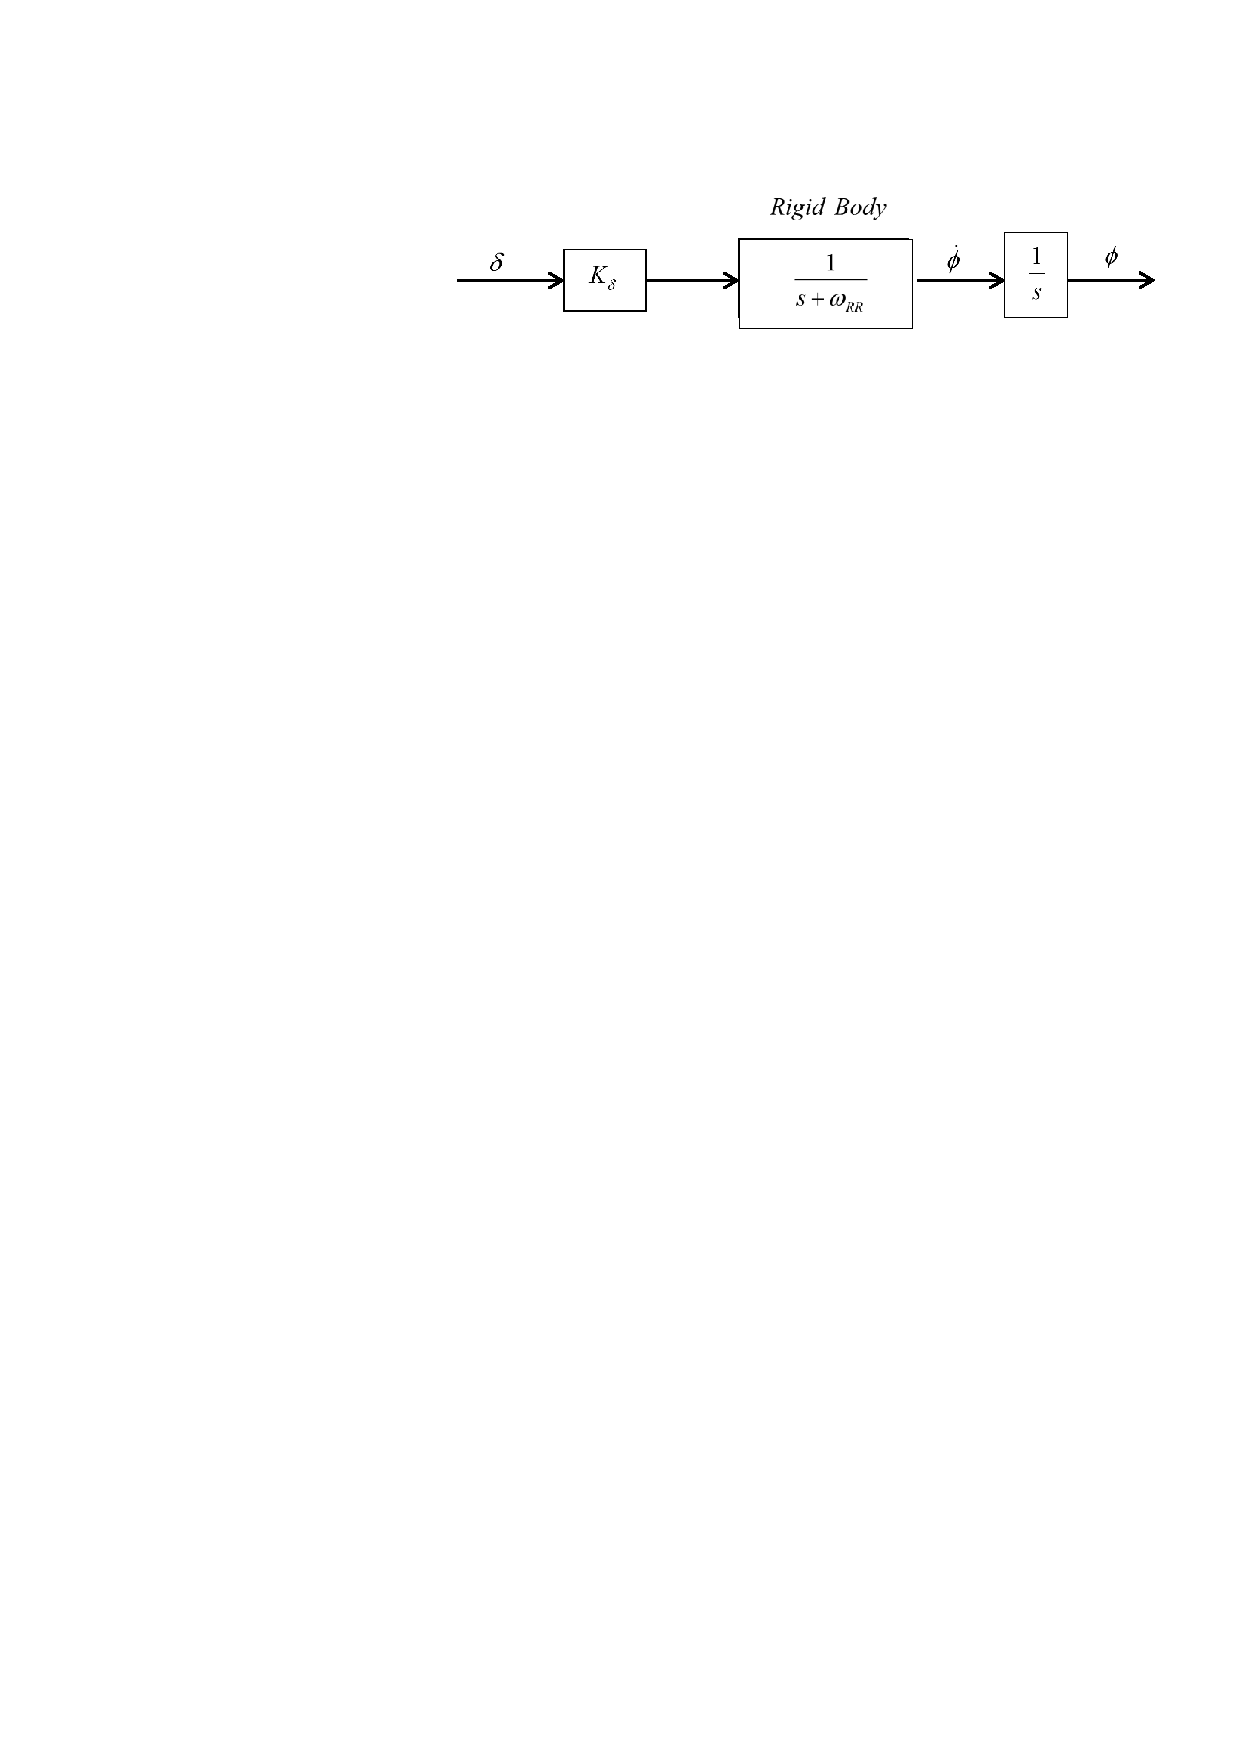
\includegraphics[width=0.8\linewidth]{fig1}
	\end{figure}
	\begin{itemize}  % Shows text in bullet point 		
		\item ADD
		\item ADD
			%\begin{enumerate}
				%\item $x_1=\phi$
				%\item $x_2=p$
			%\end{ enumerate}
		\item ADD TABLE ALSO AFTER OR BEFORE THIS...WHERE EVER TO INDICATE WHAT THE TERMS MEAN
	\end{itemize}
	%\textbf{}
	%
	%Assuming rigid body dynamics, the linearized roll dynamics for a tactical missile can be represented as
 		 %%
%\begin{equation}
%\frac{\phi(s)}{\delta(s)} = \frac{K_{\delta}}{s(s + \omega_{RR})}
%\label{eq1}
%\end{equation}
%%
\end{frame}

%------------------------------------------------
%SUBSECTION1
\subsection{Controller Design} % A subsection can be created just before a set of slides with a common theme to further break down your presentation into chunks

% Start of Fourth slide
%\begin{frame}[shrink]
	%\frametitle{Design of UDE based control law assuming ideal actuator}
	%\textbf{Plant dynamics in state space form} 	
 	%\begin{itemize}  % Shows text in bullet point 		
		%\item Since an ideal actuator has been assumed, $\delta=\delta_c$
		%\item $\phi$ = roll angle in deg
			%%\begin{enumerate}
				%%\item $x_1=\phi$
				%%\item $x_2=p$
			%%\end{ enumerate}
		%\item $p$ = roll rate in deg/s
	%\end{itemize}
	 		%%
%Assuming uncertainties in $\omega_{RR}$ and $K_\delta$, 
%\begin{eqnarray*}
%\dot{x}_1 &=& x_2 \nonumber \\
%\dot{x}_2 &=& -( \omega_{RRn} + \Delta\omega_{RR})x_2 + (K_{\delta n} + \Delta K_{\delta} )\delta + d'
%\label{eq3}
%\end{eqnarray*}
%%
%Clubbing the uncertainties and disturbance terms and defining $d = -\Delta\omega_{RR}x_2 + \Delta K_{\delta} \delta + d'$
%%
%\begin{eqnarray*}
%\dot{x}_1 &=& x_2 \nonumber \\
%\dot{x}_2 &=& - \omega_{RRn}x_2 + K_{\delta n}\delta + d
%\label{eq4}
%\end{eqnarray*}
%%
%With $\delta$ as the control input ($u$), the following control law is proposed 
%%
%\begin{equation*}
%u = \frac{1}{K_{\delta n}}\left[u_a + u_d + \nu \right]
%\label{eq5}
%\end{equation*}
%%
%\end{frame}
%-------------------------option2-----------------------------------------------------------------------------------------------------------
\begin{frame}
	\frametitle{Input Output Linearization}
	\textbf{Plant dynamics in state space form} 
	\begin{itemize}
		\item Trip Diff
		\item $d_n \approx 0$ -- relative degree
		\item alpha constraints
	\end{itemize}
	
\begin{eqnarray*}
\begin{aligned}
	\dddot{\alpha}&=K_q M^2(3a_m\alpha^2+2b_m|\alpha|+c_m\Big(-7+\frac{8M}{3}\Big))\dot{\alpha}\\ 
	&\quad - K_q M^2d_m\omega_a\delta+K_{\alpha}M(6a_n\alpha+2b_n sgn(\alpha))\dot{\alpha}^2\\ 
	&\quad + K_\alpha M(3a_n\alpha^2+2b_n|\alpha|+c_n\Big(2-\frac{M}{3}\Big))\ddot{\alpha}\\ 
	&\quad + K_q M^2d_m\omega_a\delta_c \label{a3dot}
\end{aligned}
\label{eq4}
\end{eqnarray*}

where to get the form al-trip-dot = a + bu, 
\end{frame}

\begin{frame}
\begin{eqnarray*}
	\begin{aligned}
		a &= K_qM^2(3a_m\alpha^2+2b_m|\alpha|+c_m\Big(-7+\frac{8M}{3}\Big))\dot{\alpha} \\ 
		&\quad -K_qM^2d_m\omega_a\delta+K_\alpha M(6a_n\alpha+2b_nsgn(\alpha))\dot{\alpha}^2\\ 
		&\quad+K_\alpha M(3a_n\alpha^2+2b_n|\alpha|+c_n\Big(2-\frac{M}{3}\Big))\ddot{\alpha} \\
		b &= K_q M^2d_m\omega_a \nonumber
	\end{aligned}
	\label{eq5}
\end{eqnarray*}


Thus, 

\begin{eqnarray*}
	\begin{aligned}
%		without this comment the equations on this slide disappear. No idea why.
		\delta_c &= \frac{1}{b}(u_a+\nu) \\ \label{iol_control}
		u_a &= -a \label{ua_eqn}\\
		\nu &= \dddot{\alpha}^\ast+m_1(\alpha^\ast-\alpha) + m_2(\dot{\alpha}^\ast-\dot{\alpha}) + m_3(\ddot{\alpha}^\ast-\ddot{\alpha}) \label{nu_eqn}
	\end{aligned}
	\label{eq5}
\end{eqnarray*}

\end{frame}
%-------------------------------------------------------------------------------------------------------------------------------------------
\begin{frame}
\frametitle{UDE Augmented IOL Controller}
\textbf{Defining $u_a$, $\nu$ and $u_d$}
%As per the uncertainty and disturbance estimator (UDE) approach, we need to define $u_a$ to take care of negating the effect of the 
\begin{itemize}  % Shows text in bullet point 		
		\item $\delta_c = \frac{1}{b}\Big[u_a+u_d+\nu\Big] $
		\item $\dddot{\alpha}=(a + \Delta a) + (b + \Delta b)\delta_c + w \nonumber$
				\begin{enumerate}
					\item $d = \Delta a + \Delta b \delta_c + w$
					\item $\dddot{\alpha} = a + b\delta_c + d \nonumber$ 
				\end{enumerate}
		\item To define $u_d$
				\begin{enumerate}
					\item $\hat{d}=G_f(s)d$
					\item $G_f(s)=\frac{1}{1+s\tau}$ \\
					we finally get
					\item $u_d=\frac{-1}{\tau}\Big[\ddot{\alpha}-\int{\nu dt}\Big] \label{ude}$
				\end{enumerate}
\end{itemize}
\end{frame}
%%------------------------------------------------------------------------------------------------------------------------------------------
\begin{frame}
\frametitle{UDE Observer based Control law}
	\textbf{The final UDE based control law using the expressions for $u_a$, $\nu$ and $u_d$}

\begin{eqnarray*}
	\begin{aligned}
		%		without this comment the equations on this slide disappear. No idea why.
		\dddot{\alpha} &= a_1 \alpha + a_2 \dot{\alpha} + a_3 \ddot{\alpha} + d_1 + b\delta_c \\
	\end{aligned}
\label{eq5}
\end{eqnarray*}

d1 = non-linear terms, a1 is coeffs alpha, a2 is coeffs alpha-dot, a3 is coeffs alpha-ddot \\

Now,

\begin{eqnarray*}
	\begin{aligned}
		\dddot{\alpha} &= a_{1o} \alpha + a_{2o} \dot{\alpha} + a_{3o} \ddot{\alpha} + b_o\delta_c + d_2\\
	\end{aligned}
	\label{eq5}
\end{eqnarray*}


%For this controller and plant system, the phase margin was found to be 69 deg, validating the proposed control law.
\end{frame}

\begin{frame}
\frametitle{UDE Observer based Control law}

\begin{eqnarray*}
	\begin{aligned}
		\dot{x}_1 &= x_2 \\
		\dot{x}_2 &= x_3 \\
		\dot{x}_3 &= a_{1o}x_1 + a_{2o}x_2 + a_{3o}x_3 + b_o \delta_c + d_2 \\
		y &= x_1 \label{rx1}
	\end{aligned}
	\label{eq5}
\end{eqnarray*}

Intro with observer poles we get

\begin{eqnarray*}
	\begin{aligned}
		\dot{\hat{x}}_1 &= \hat{x}_2 + \beta_1 e_o\\
		\dot{\hat{x}}_2 &= \hat{x}_3 + \beta_2 e_o\\
		\dot{\hat{x}}_3 &= a_{1o}\hat{x}_1 + a_{2o}\hat{x}_2 + a_{3o}\hat{x}_3 + b \delta_c + \hat{d}_2 + \beta_3 e_o\\		
		\hat{y} &= \hat{x}_1 \label{ss1}
	\end{aligned}
	\label{eq5}
\end{eqnarray*}

\end{frame}



\begin{frame}
\frametitle{Stability Analysis}

quick points

\end{frame}


%%--------------------------------------------- --
%% Start of fifth slide
\subsection{Performance of UDE based controller}
\begin{frame}
\frametitle{Parameters used in roll dynamics}
\textbf{Simulation Parameters as referred from \cite{talole2011}}
%
\begin{table}[h]
\begin{center}
\caption{Performance specifications}\label{tb1}
\begin{tabular}{ccc}
\hline
$\omega_{RRn}$ & roll rate bandwidth & 2 rad/s\\ \hline
$K_\delta n$ & fin effectiveness & 9000 1/$s^2$\\ \hline
$\omega_A$ & actuator bandwidth & 100 rad/s\\ \hline
$\zeta_A$ & actuator damping & 0.65 \\ \hline
$\phi_{max}$ & maximum desired roll angle & 10 deg\\ \hline
$\dot{\phi}_{max}$ & maximum desired roll rate & 300 deg/s\\ \hline
$d_{ext}$ & external disturbance & 200 rad/$s^2$ \\ \hline
$\delta_{cmax}$ & maximum desired fin deflection & 30 deg \\ \hline


%For this controller and plant system, the phase margin was found to be 69 deg, validating the proposed control law.
\end{tabular}
\end{center}
\end{table}
\end{frame}
%%------------------------------------------------------------------------------------------------------------------------------------------

\begin{frame}
\frametitle{Performance of UDE based controller}
\textbf{Parameters for simulation}
\begin{itemize}  % Shows text in bullet point 		
		\item filter constant $\tau=0.01$
		\item desired settling time $t_s= 180$ ms
		\item damping factor $\zeta = 0.8$
				\begin{enumerate}
					\item Using these values, feedback gains $m_1$ and $m_2$ were evaluated to be $m_1=42.45$, $m_2=771.13$ 
					%\item 
				\end{enumerate}
		\item external disturbance $d_{ext}= 200$ rad/$s^2$
		\item taking $\omega_{RR}$ to be -3 rad/s against the nominal value of 2 rad/s
		\item desired roll orientation $=0$ deg
		\item initial condition in $\phi= 10$ deg
		\item all other values as referred from Table.1
	\end{itemize}
	
\textbf{For this controller and plant system, the phase margin was found to be 69 deg, validating the proposed control law}
\end{frame}
%Choosing $\tau$ to be 0.01, a desired settling time of 180 ms and a damping factor of 0.8 magnitude, the feedback gains $m_1$ and $m_2$ were evaluated as 42.45 and 771.13, respectively. Referring to Table I, we assume the external disturbance of 200 rad/$s^2$ and desired roll orientation to be 0 deg. With this choice of $\tau$, simulation results while considering an initial condition of $\phi$ to be 10 deg, are shown in Fig. 2.
%%-----------------------------------------------------------------------------------------------------------------------------------------
\begin{frame}
\frametitle{Performance of UDE based controller}
%\textbf{Simulation Output}
\begin{figure}
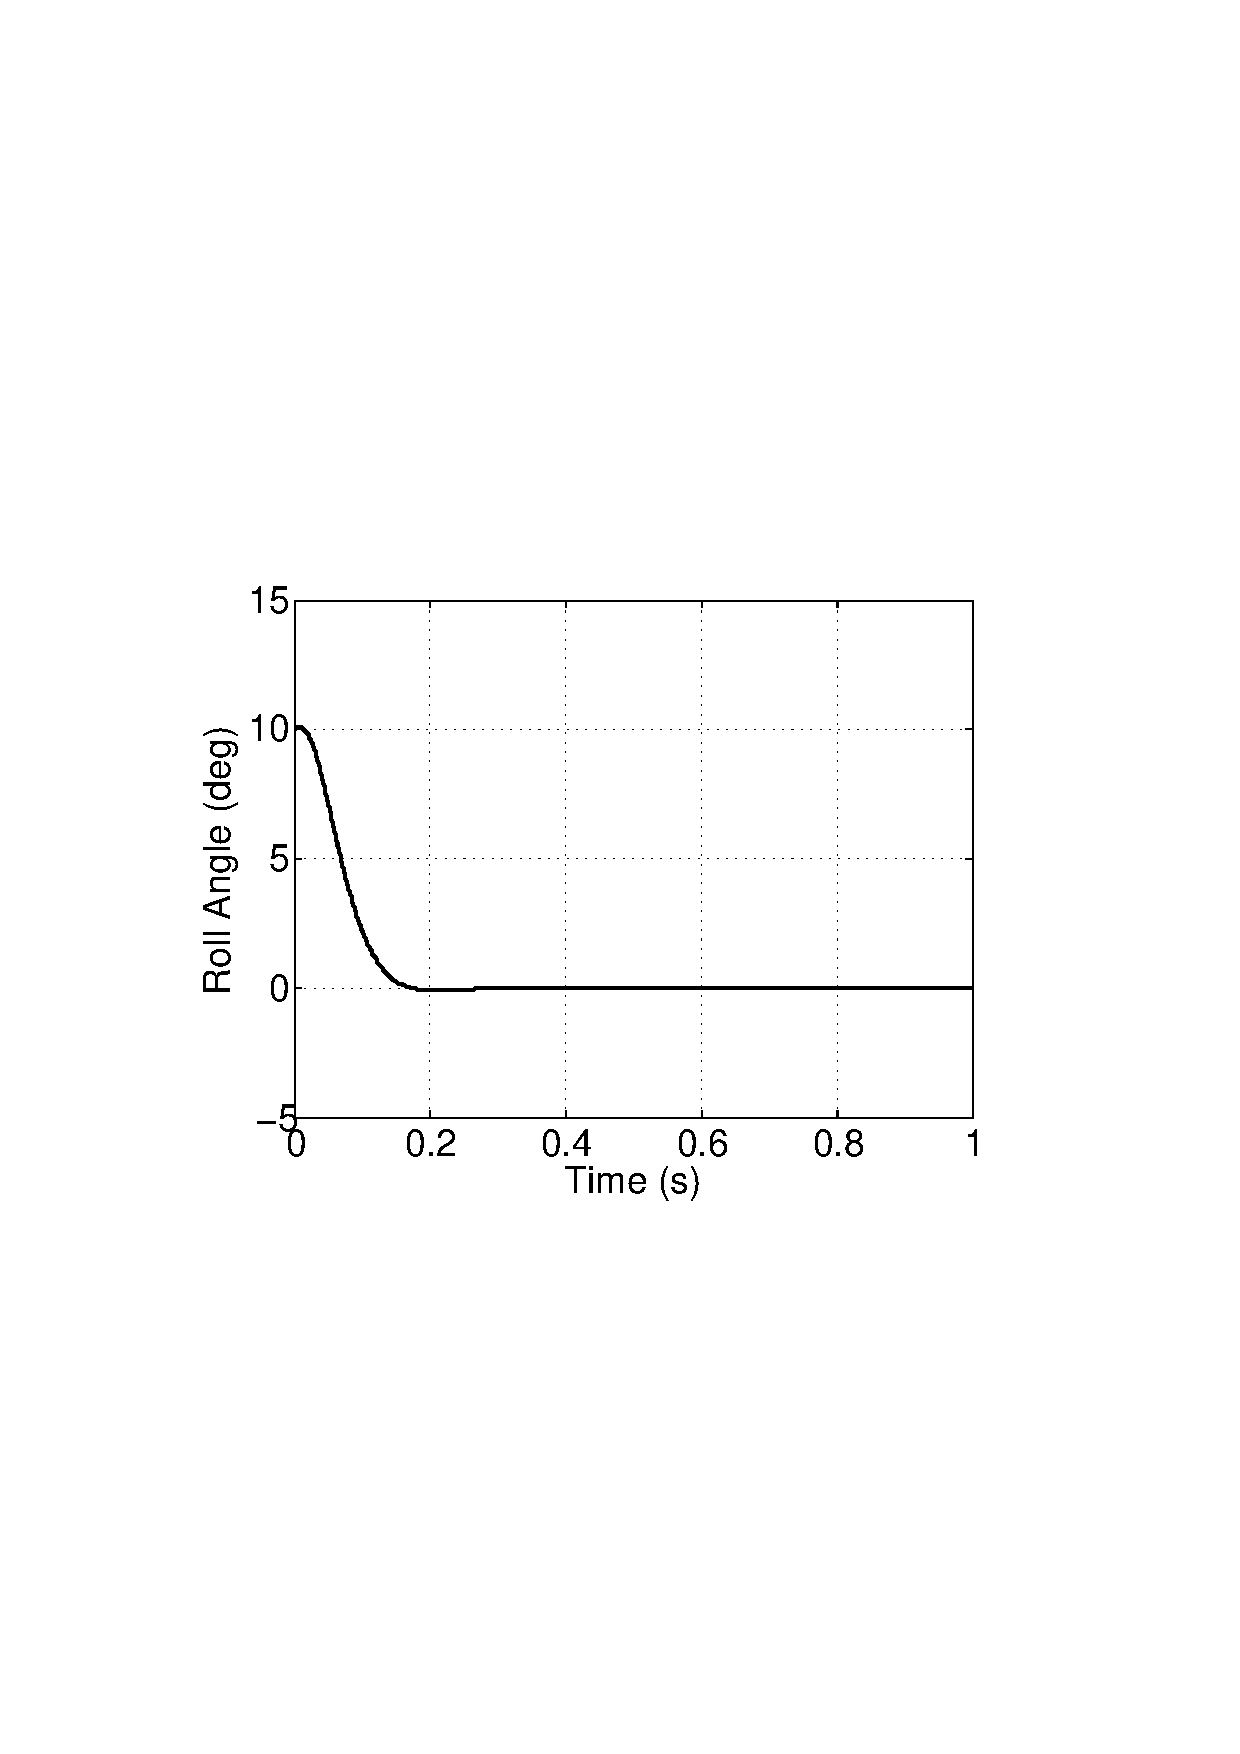
\includegraphics[width=3.7cm]{fig2a}
%\title{Output response}
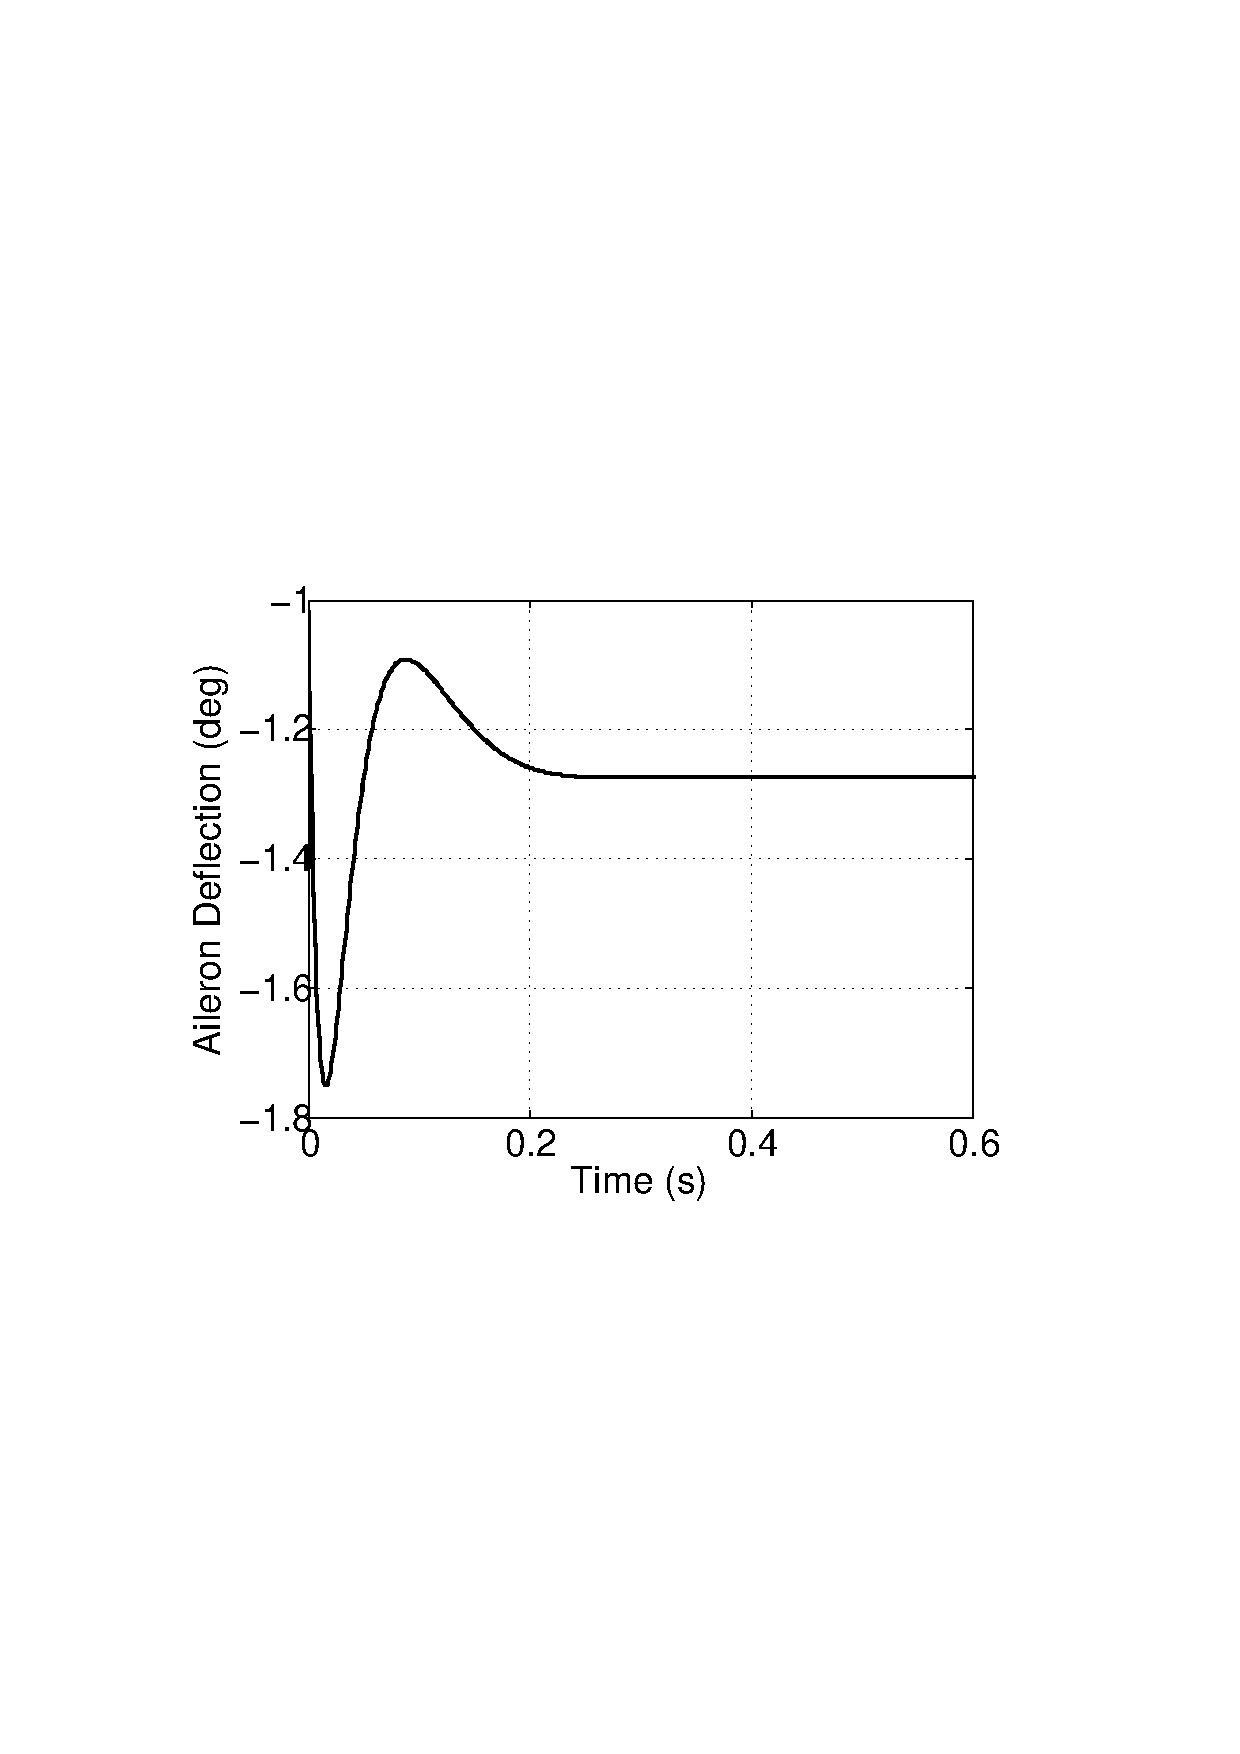
\includegraphics[width=3.7cm]{fig2b}
%\caption{Output response}
%\end{figure}
\begin{center}
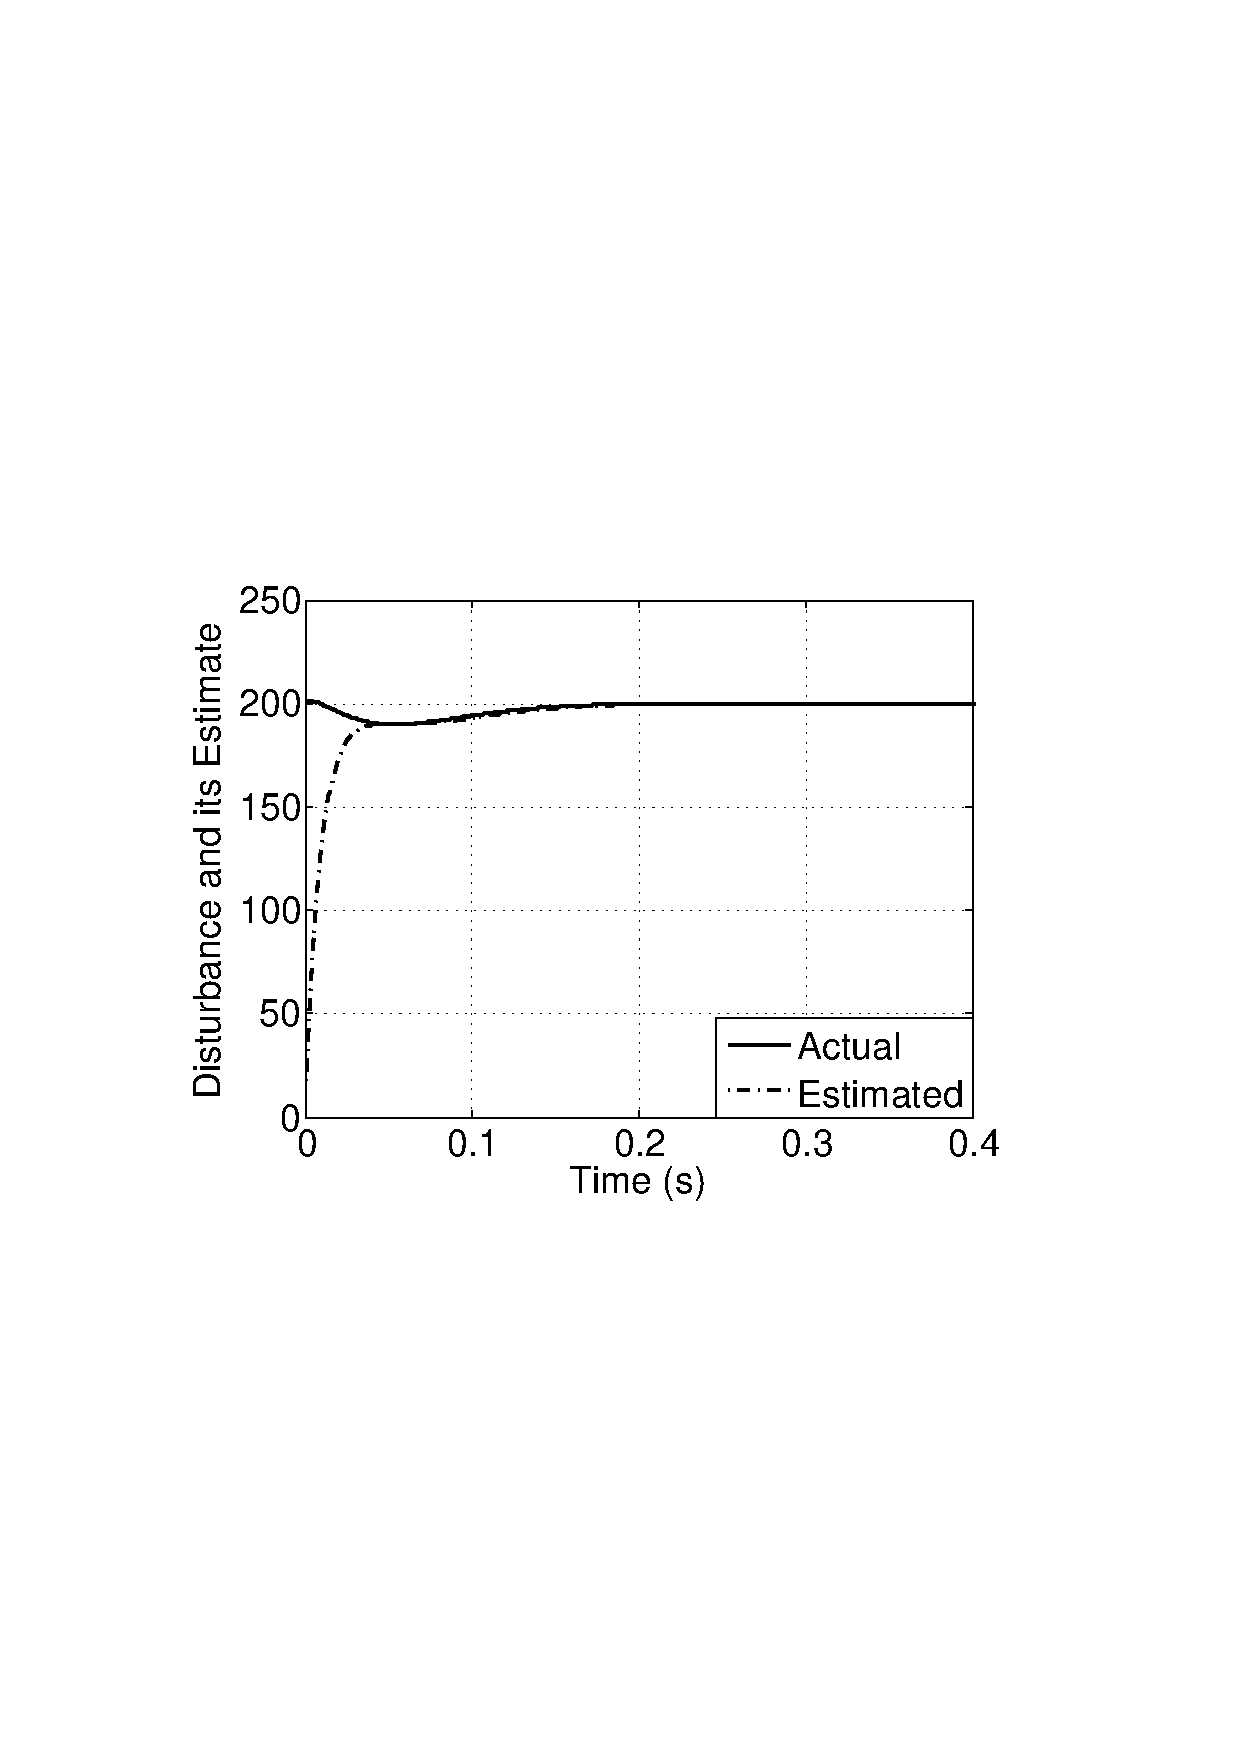
\includegraphics[width=3.7cm]{fig2c}
\end{center}
\end{figure}
%\begin{figure}
%\begin{center}
	%%%%\begin{figure}
	%%\begin{subfigure}
	%%\subfigure[Disturbance Estimation]{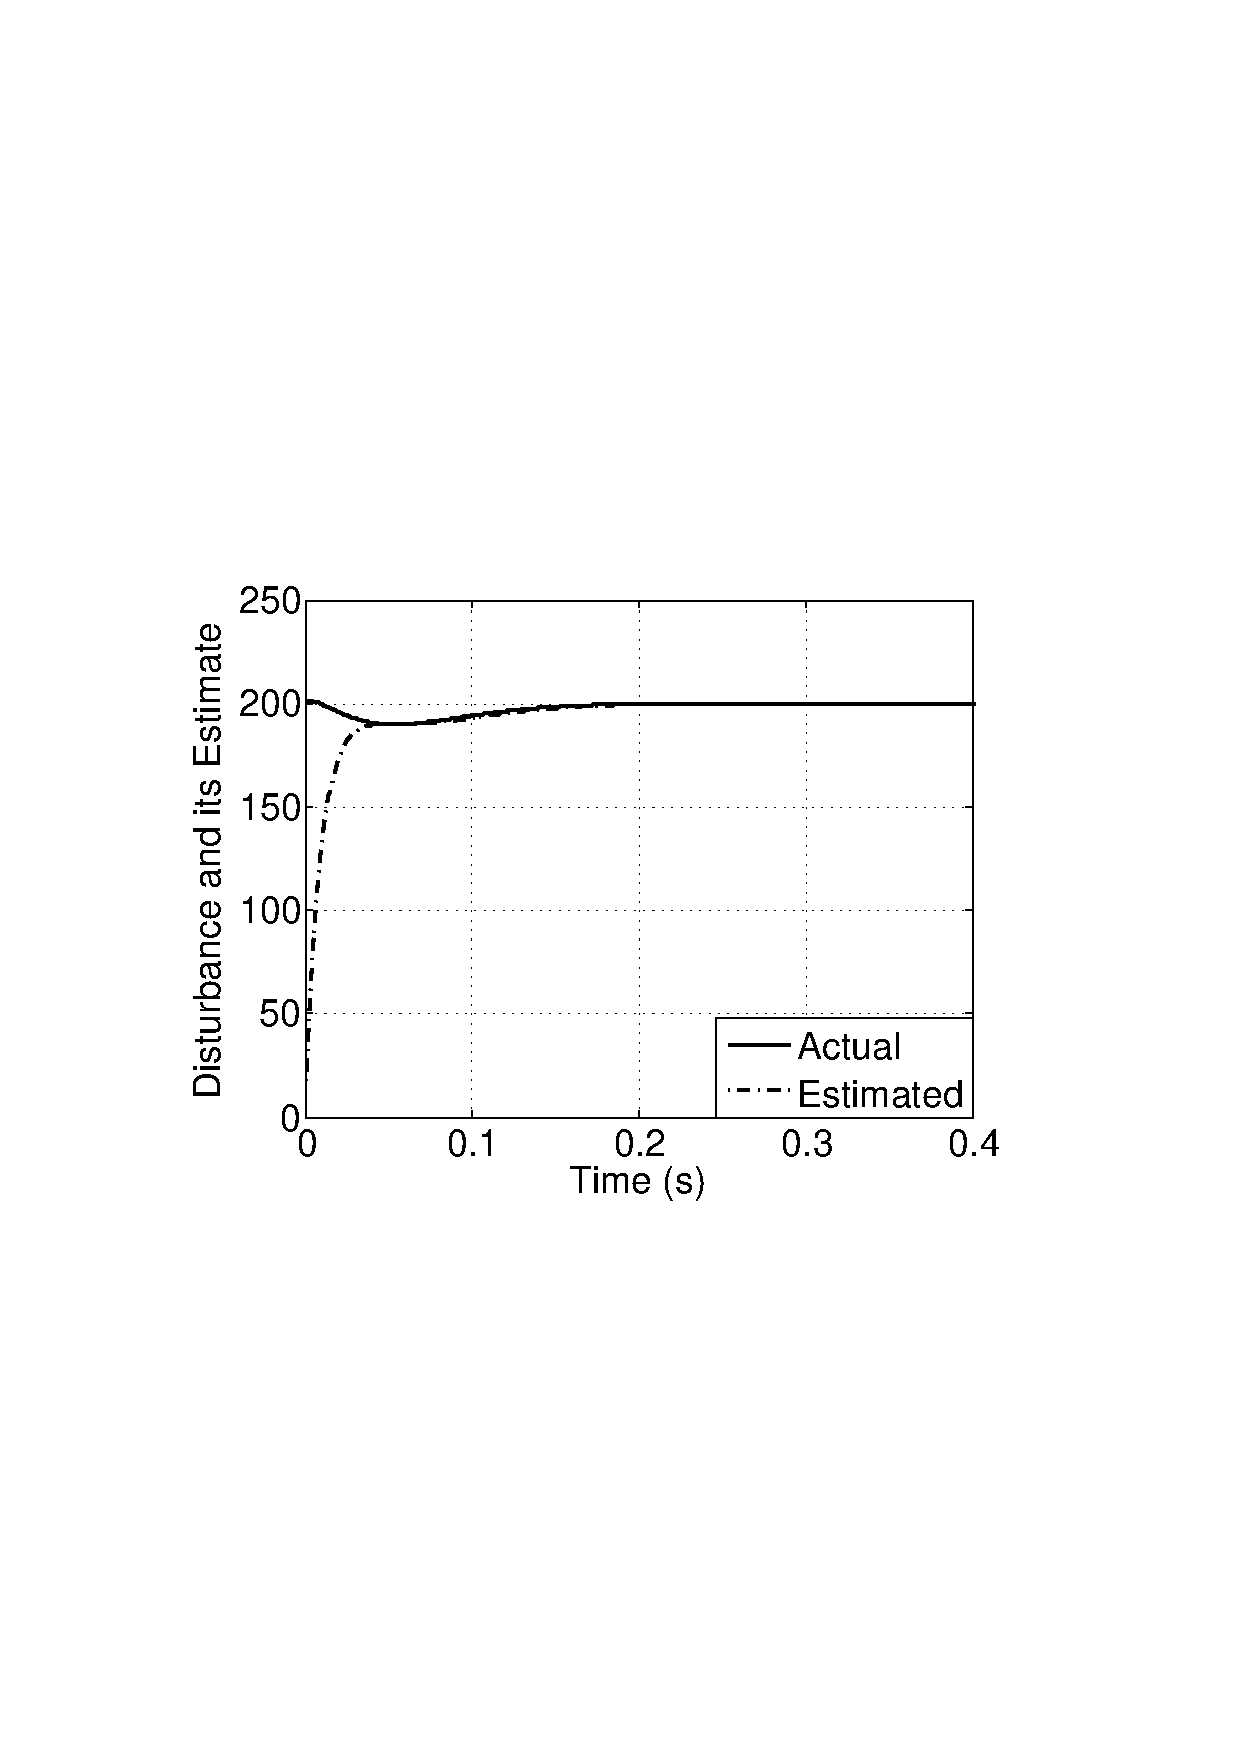
\includegraphics[width=4cm]{fig2c}
	%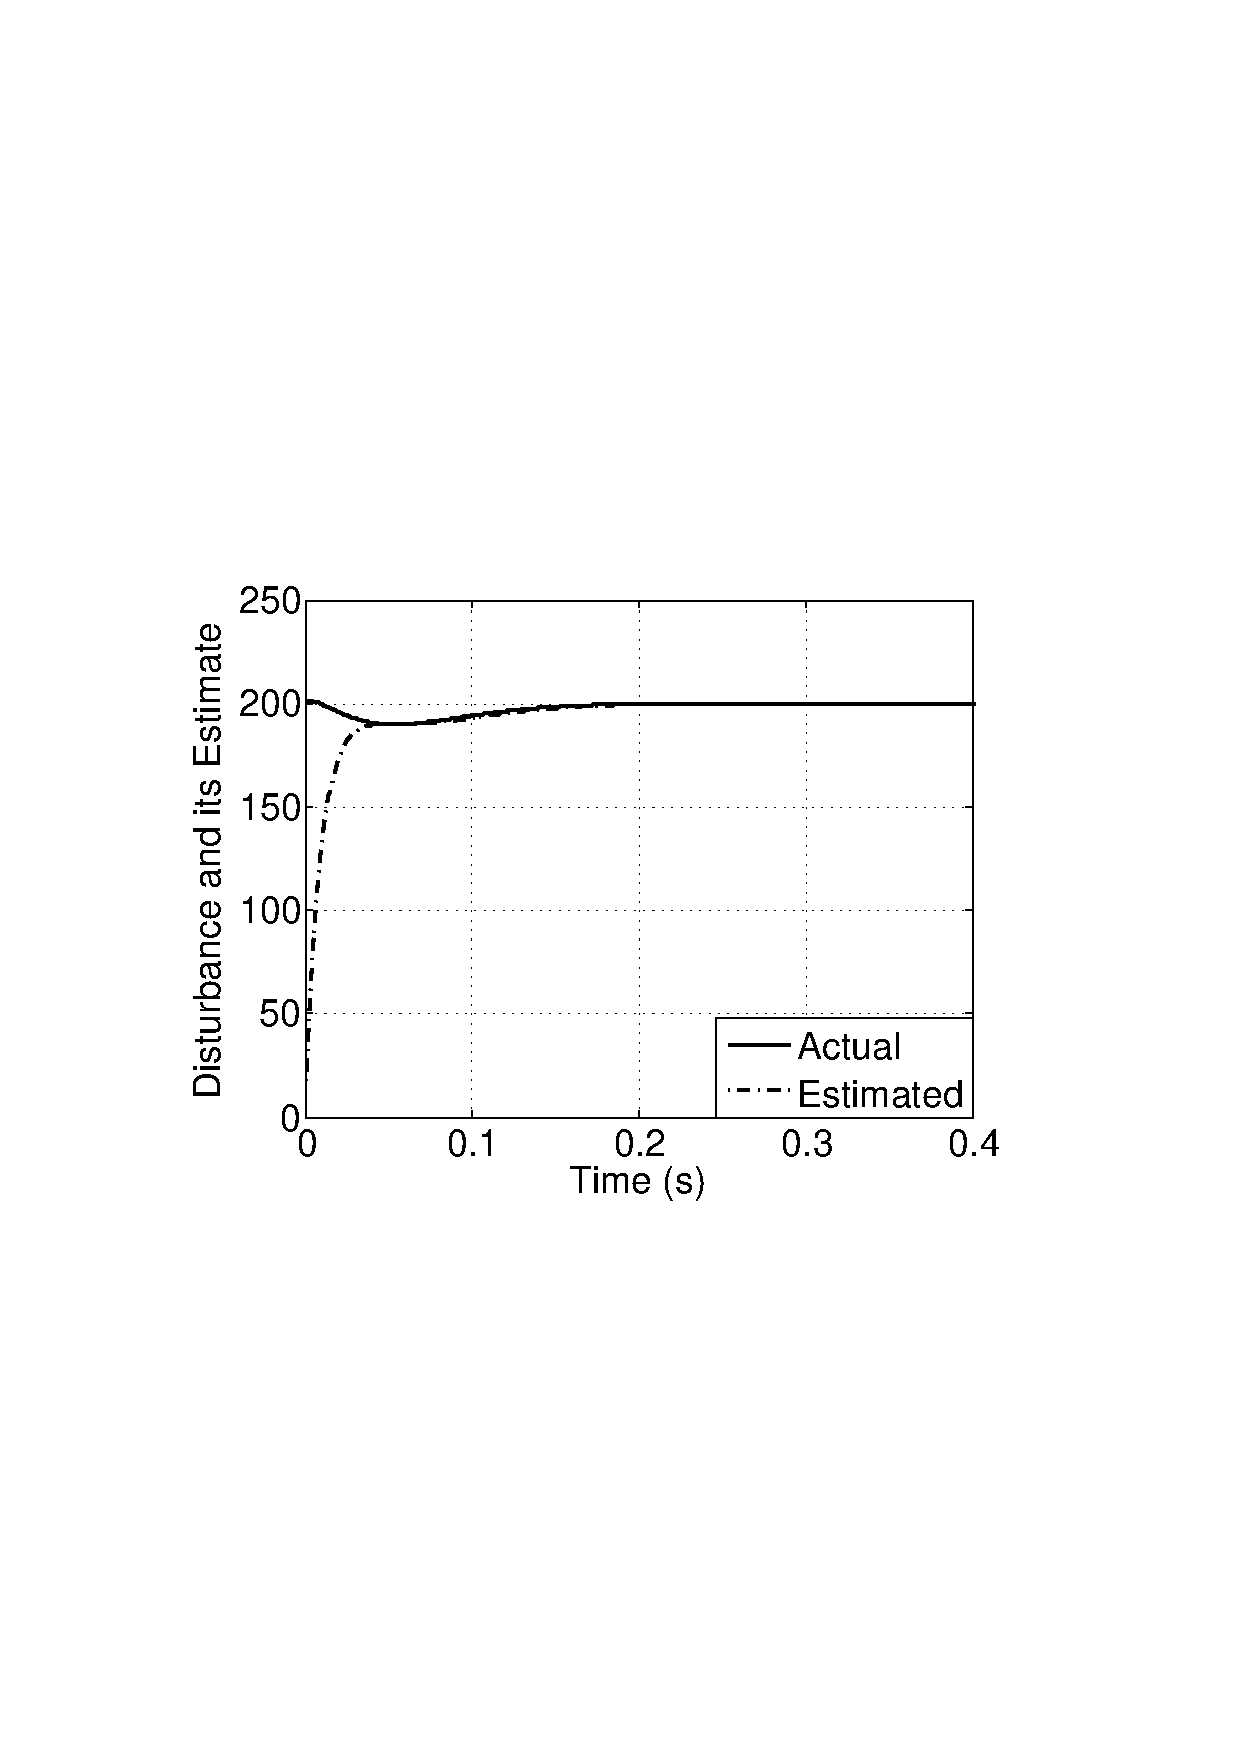
\includegraphics[width=3cm]{fig2c}
	%%\end{subfigure}
	%%\end{figure}
%\end{center}
%\end{figure}
%\begin{center}
	%\begin{subfigure}
	%\subfigure[Output Response]{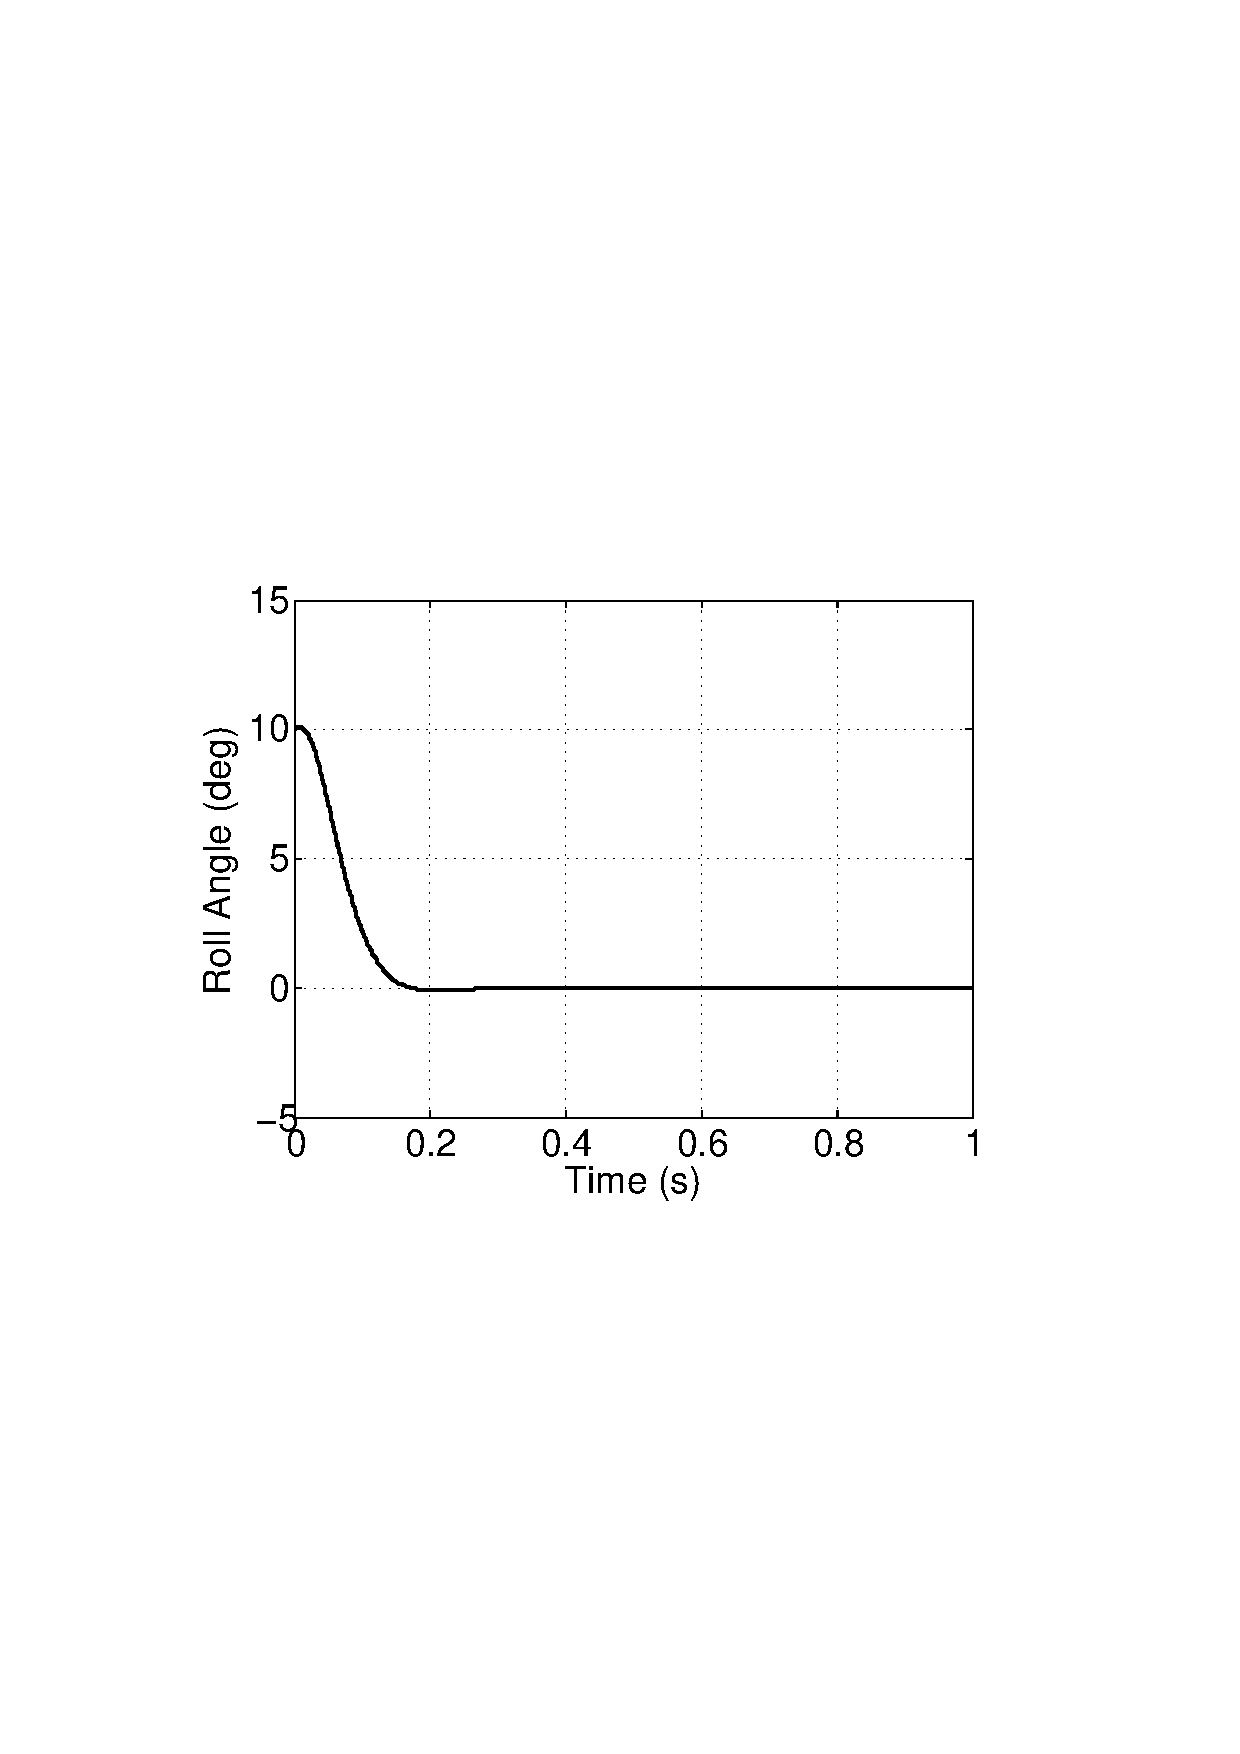
\includegraphics[width=8.4cm]{fig2a}}
	%\subfigure[Output Response]{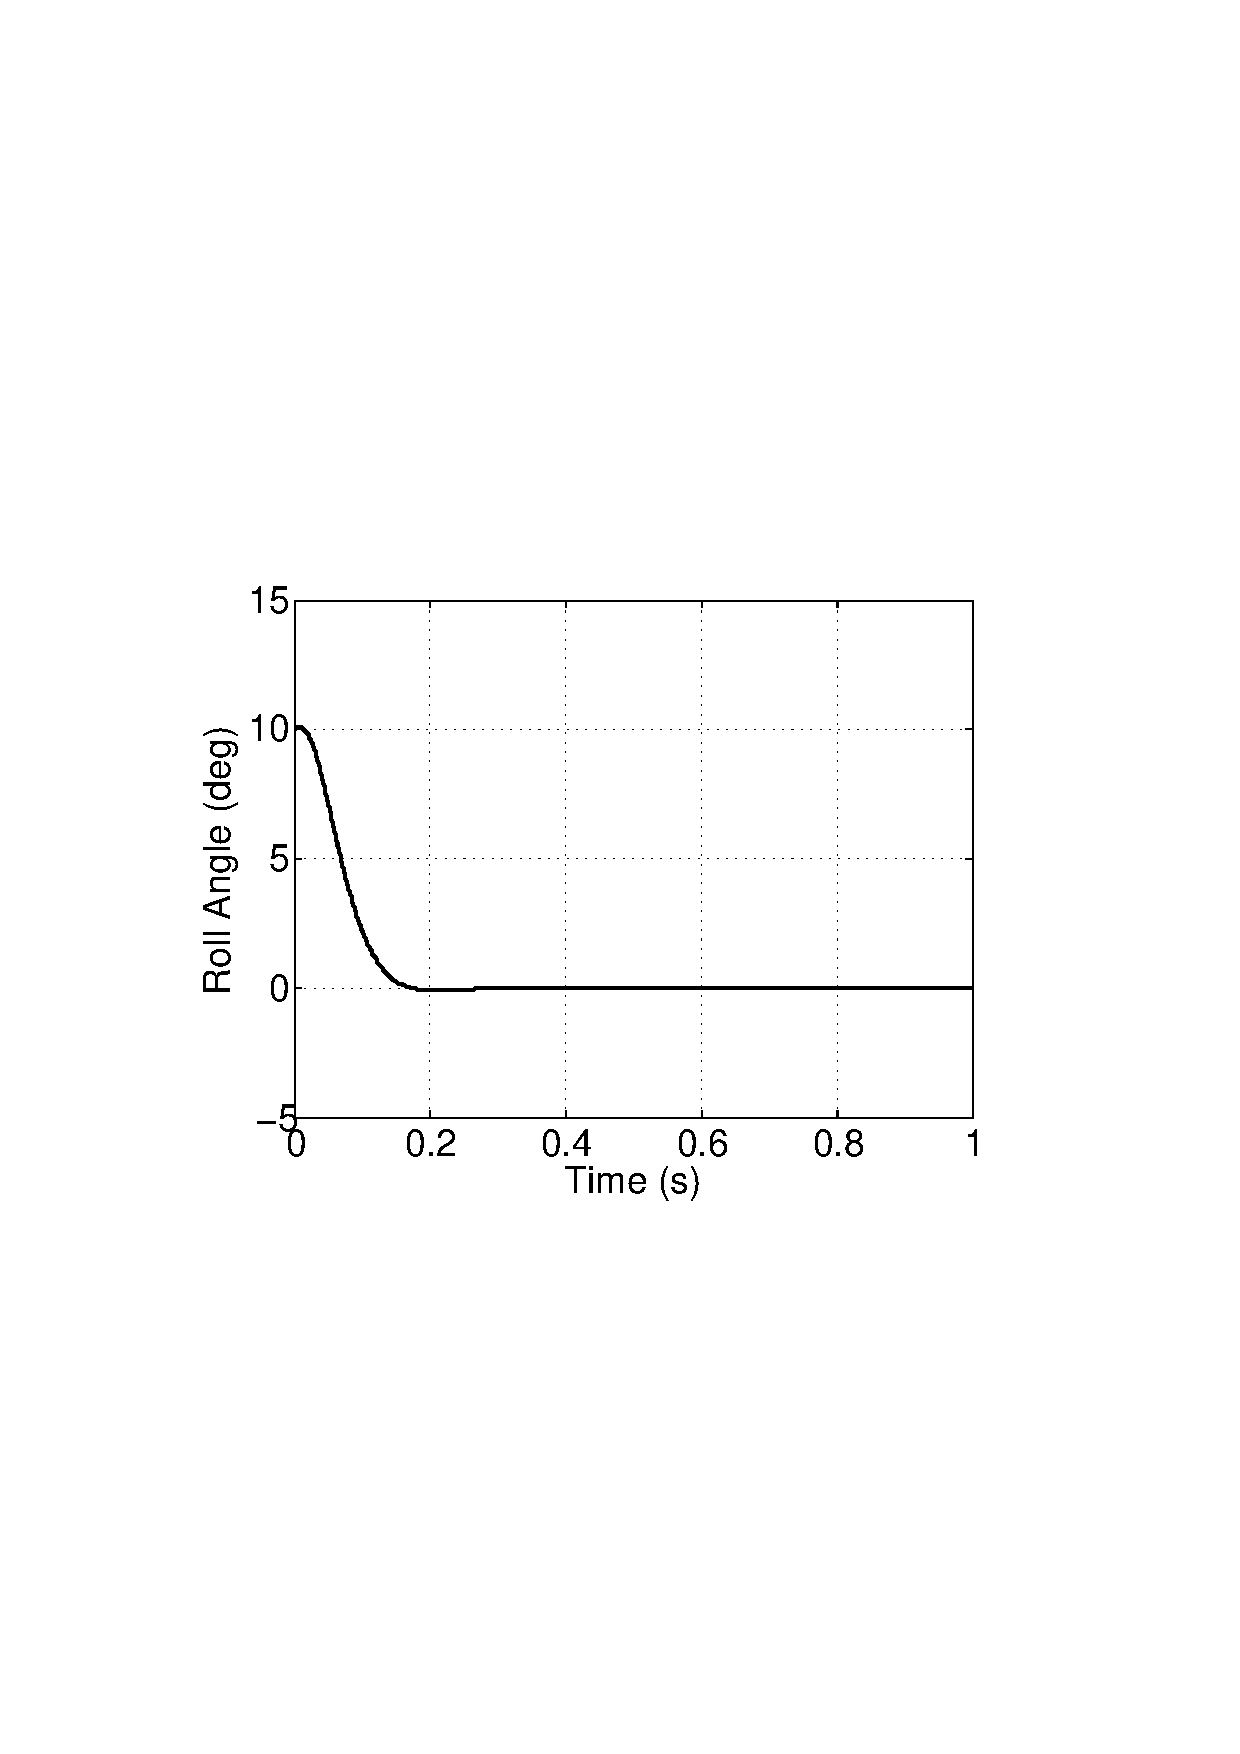
\includegraphics[width=4cm]{fig2a}}
	%%\includegraphics[width=8.4cm]{fig3a}    % The printed column width is 8.4 cm.
	%%\caption{Output response}
	%%\end{subfigure}
%%
	%%\begin{subfigure}
	%\subfigure[Control Effort]{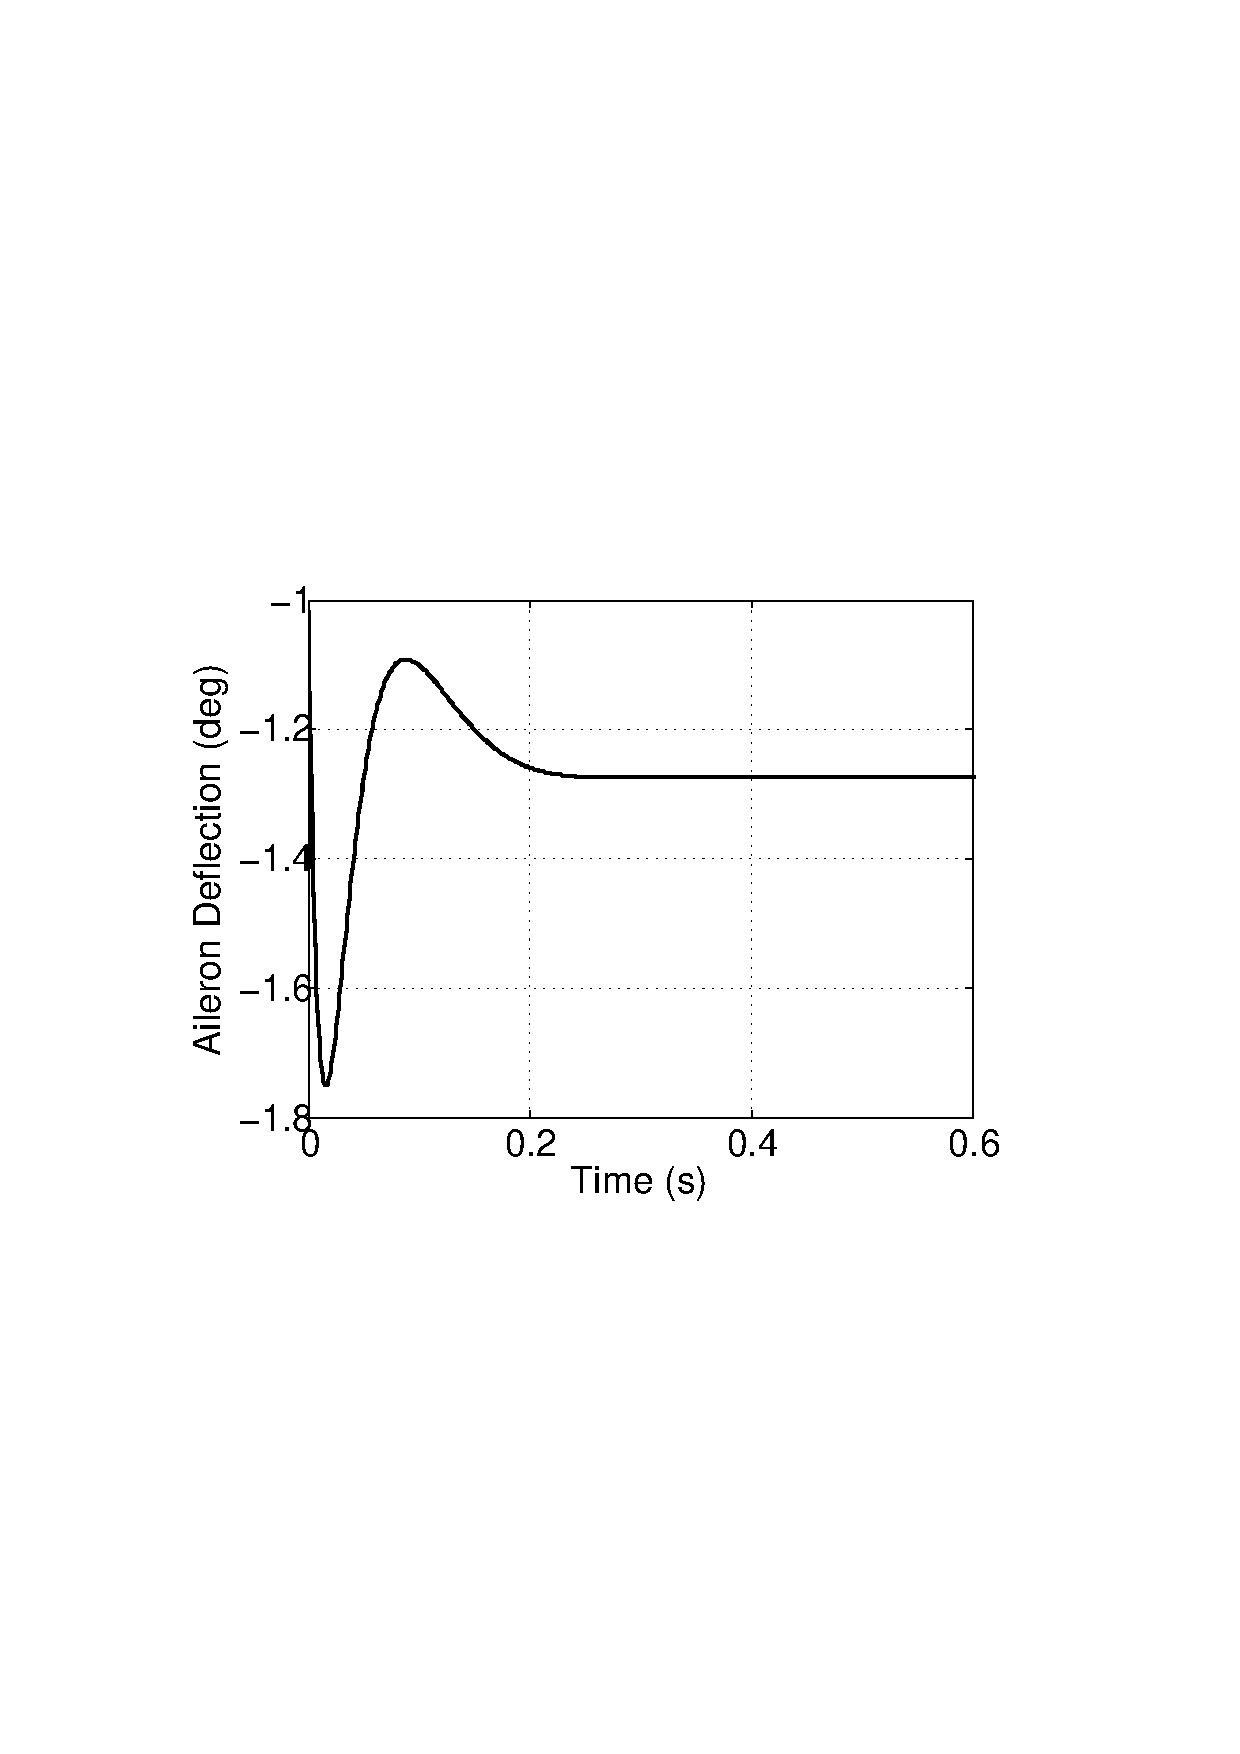
\includegraphics[width=4cm]{fig2b}}
	%%\includegraphics[width=8.4cm]{fig3b}    % The printed column width is 8.4 cm.
	%%\caption{Control Effort}
	%%\end{subfigure}
	%\subfigure[Disturbance Estimation]{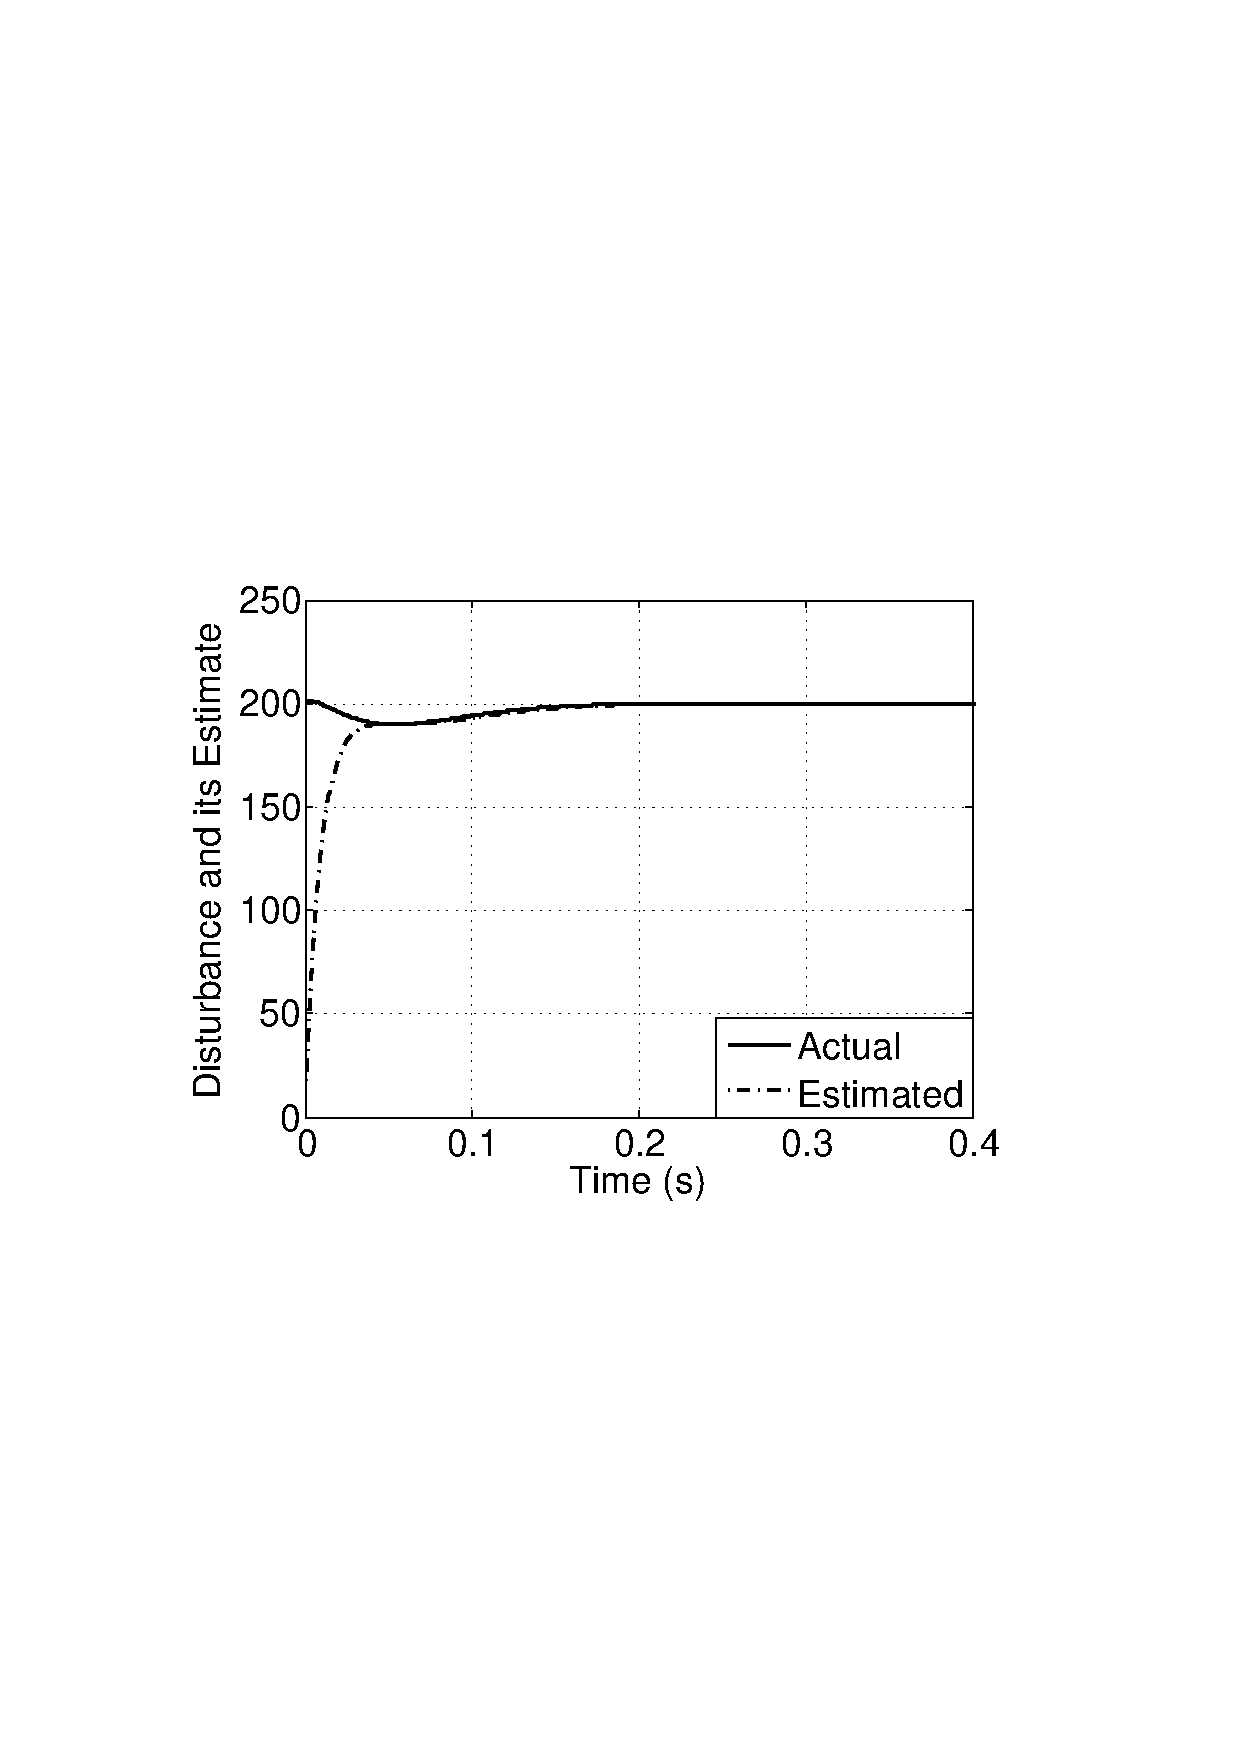
\includegraphics[width=4cm]{fig2c}}
	%\caption{Performance with UDE with ideal actuator} 
%\label{fig2}
%%\end{center}

%\end{figure}
%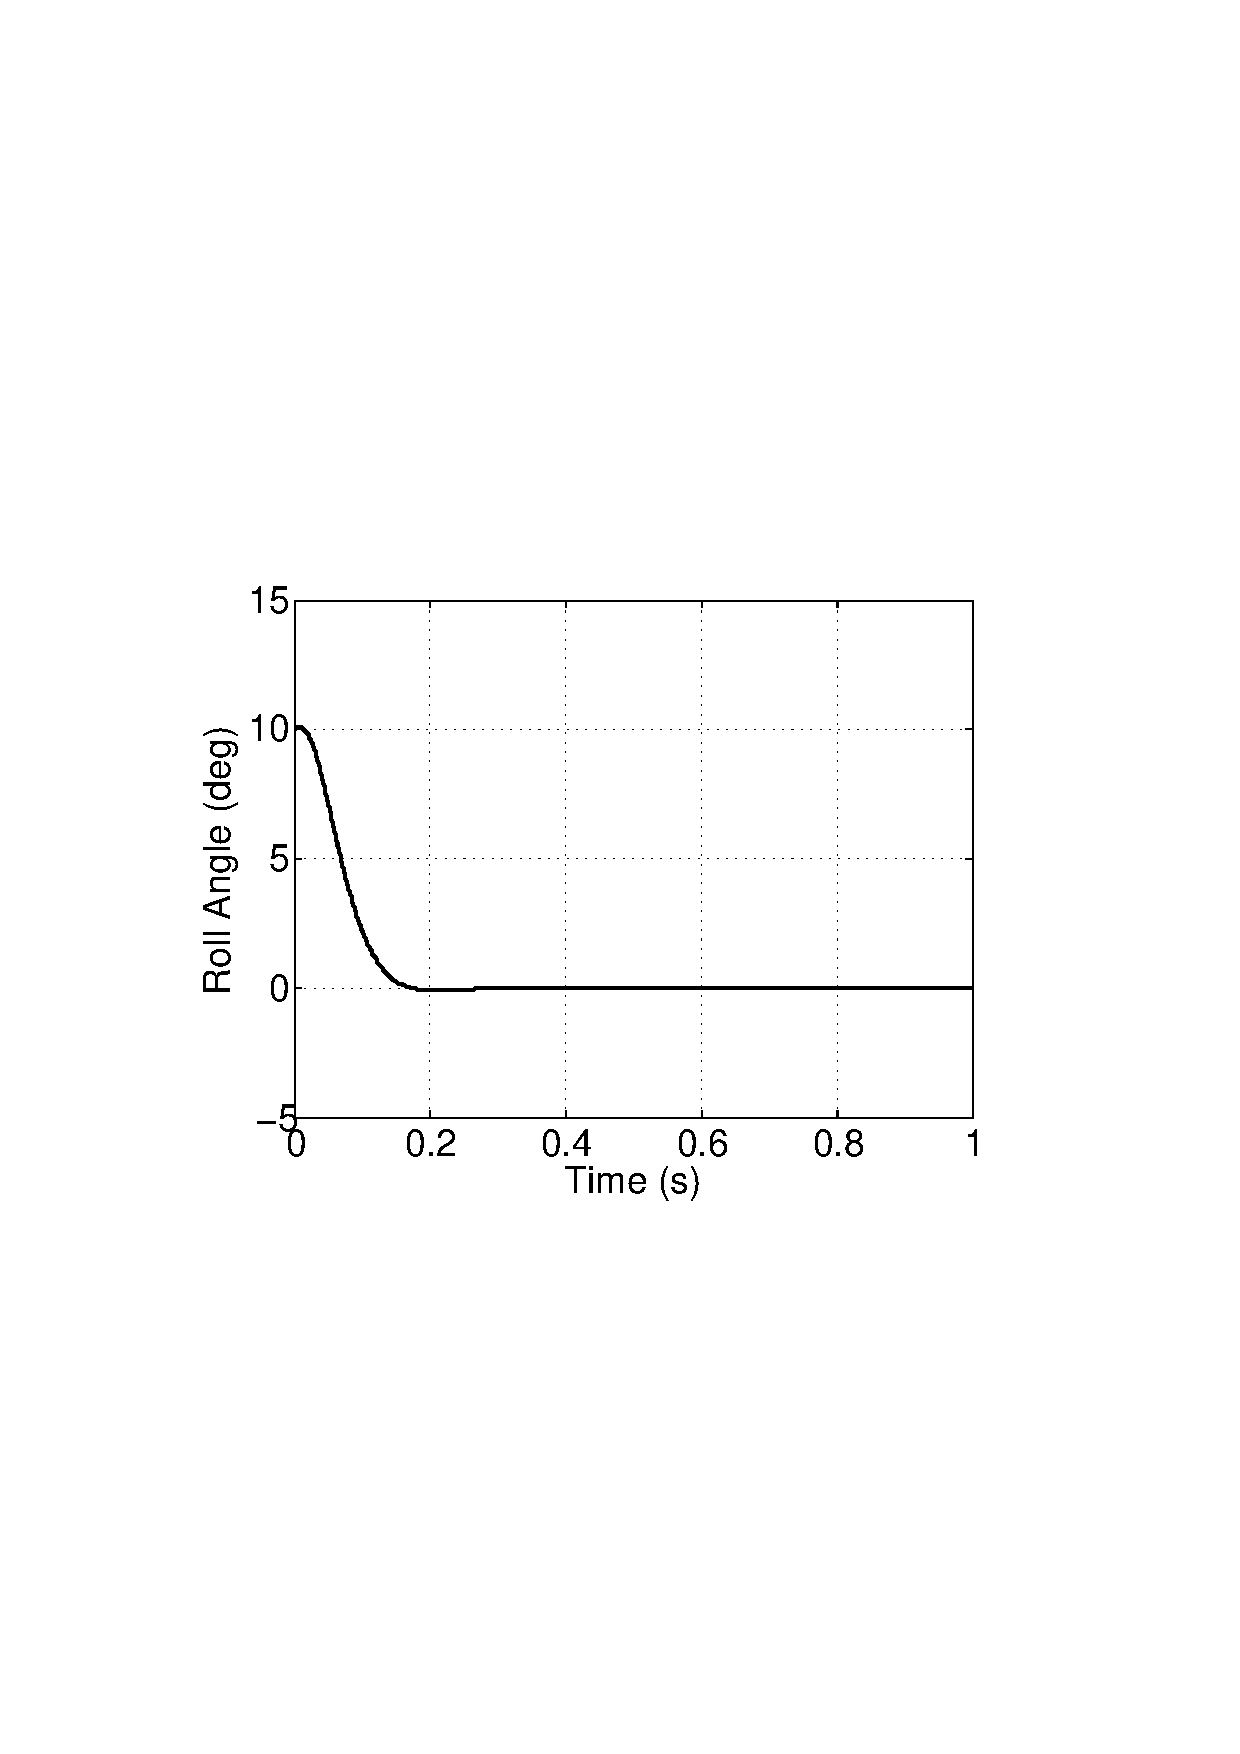
\includegraphics[width=3cm]{fig2a}
%%\caption{Output response}
%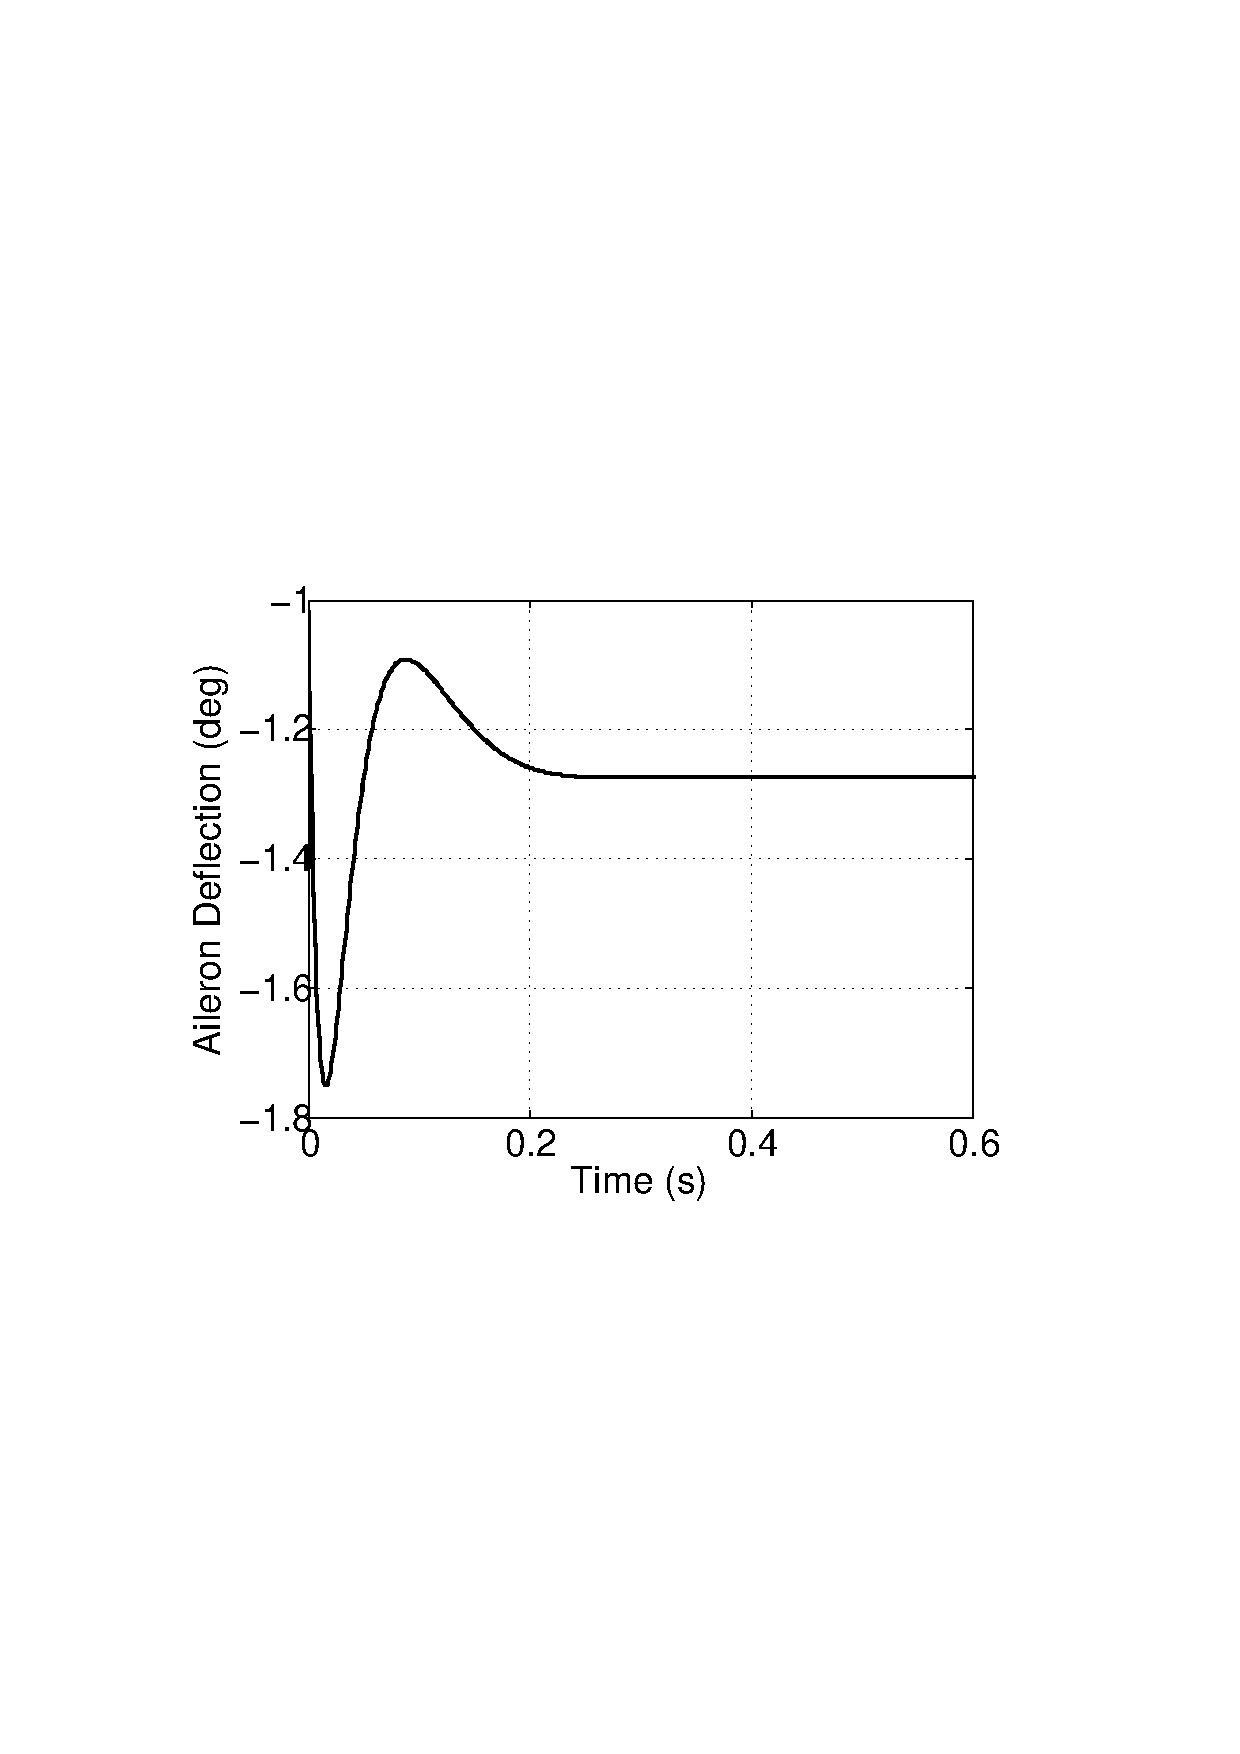
\includegraphics[width=3cm]{fig2b}
%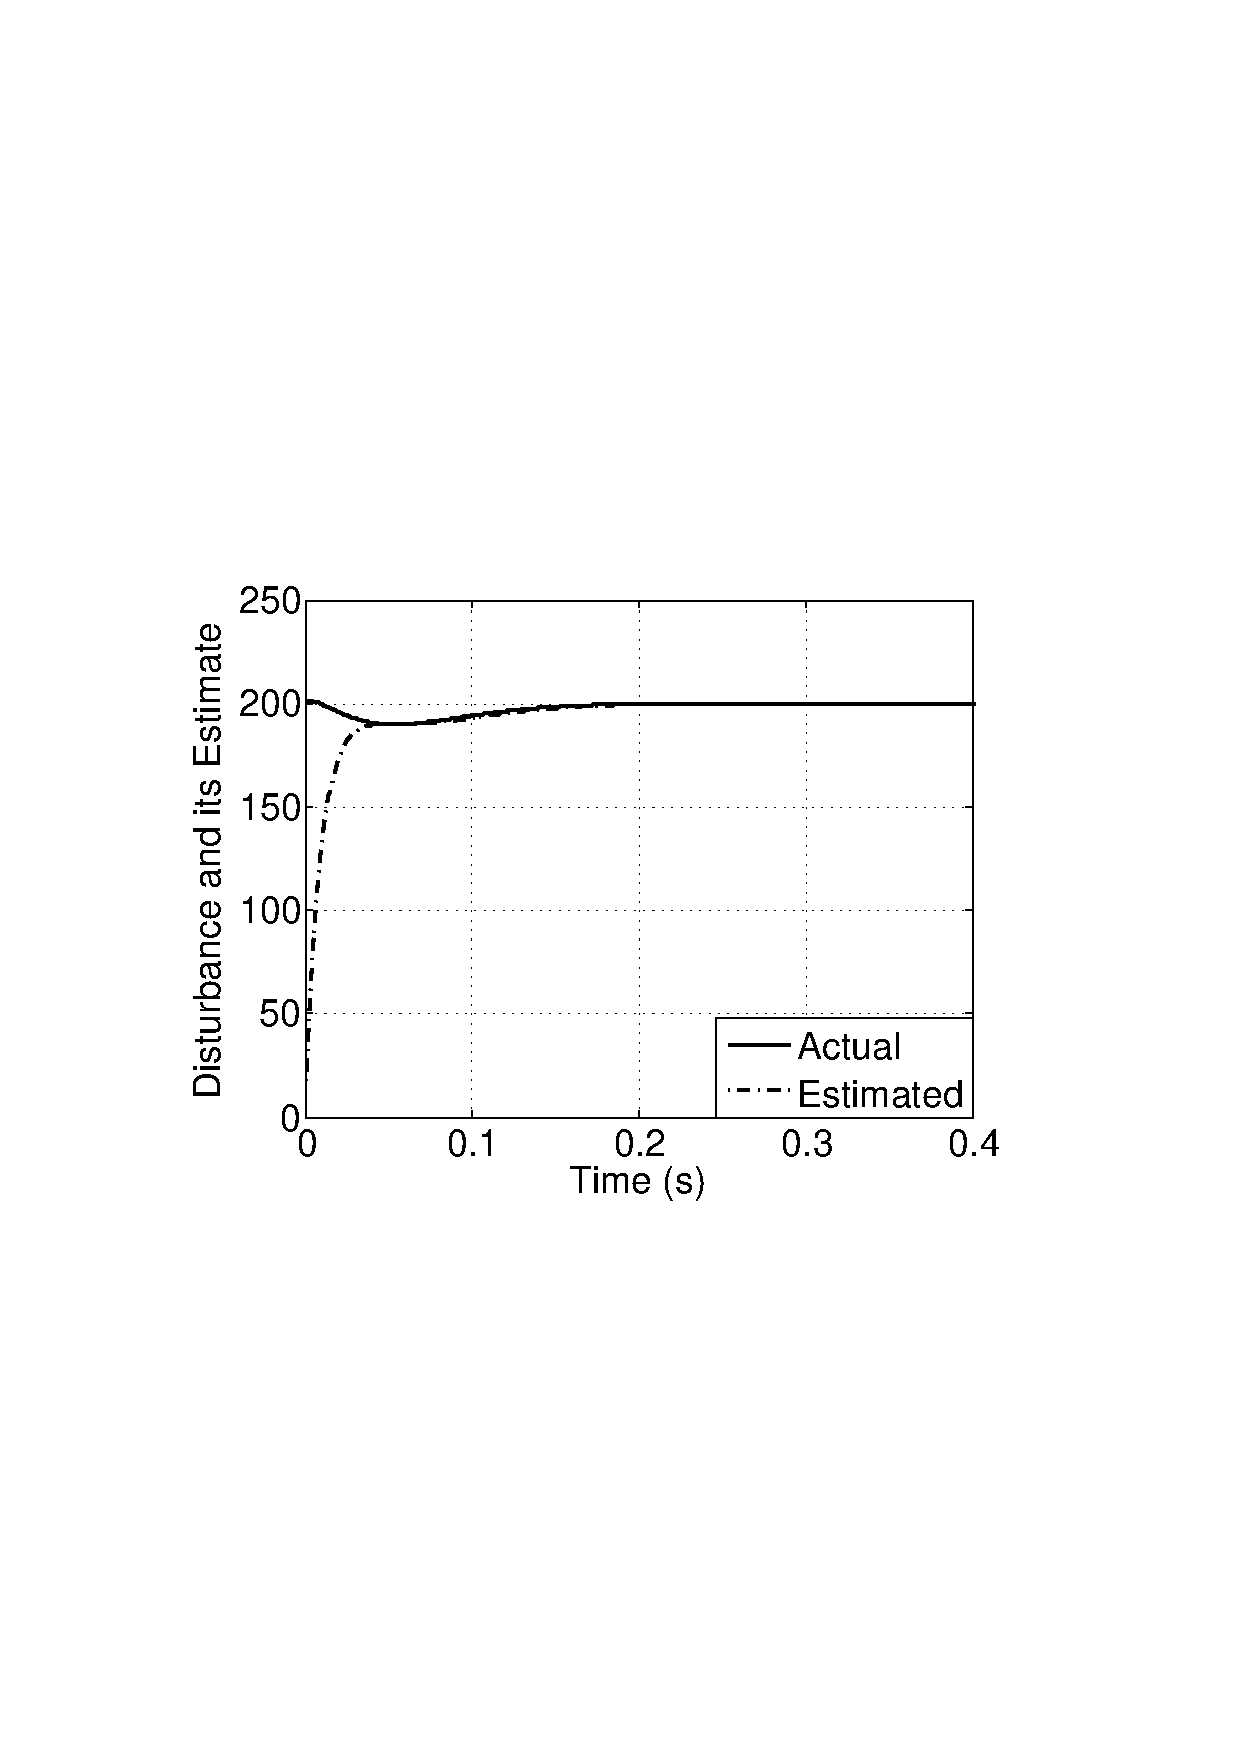
\includegraphics[width=3cm]{fig2c}

\end{frame}	
%%------------------------------------------------
%%% Start of sixth slide

\section{Performance of UDE based controller with second order actuator in the loop}
%\subsection{Without Actuator compensation}
\begin{frame}
\textbf{Cascading second order actuator}
Second order actuator as referred in \cite{talole2011} of the form ${{\delta (s)}\over{\delta_c(s)}} = {{\omega^2_A}\over{s^2 + 2\zeta_A \omega_A s + \omega^2_A}}$ is introduced
\begin{itemize}  % Shows text in bullet point 		
		\item $\omega_A$ is actuator bandwidth in rad/s 
		\item $\zeta_A$ is actuator damping ratio
		%\item damping factor $\zeta = 0.8$
				%\begin{enumerate}
					%\item Using these values, feedback gains $m_1$ and $m_2$ were evaluated to be 
					%\item $m_1=42.45$, $m_2=771.13$ 
				%\end{enumerate}
		%\item external disturbance $d_{ext}= 200$ rad/$s^2$
		%\item desired roll orientation $=0$ deg
		%\item initial condition in $\phi= 10$ deg
		%\item all other values as referred from Table.1
\end{itemize}
\begin{figure}
	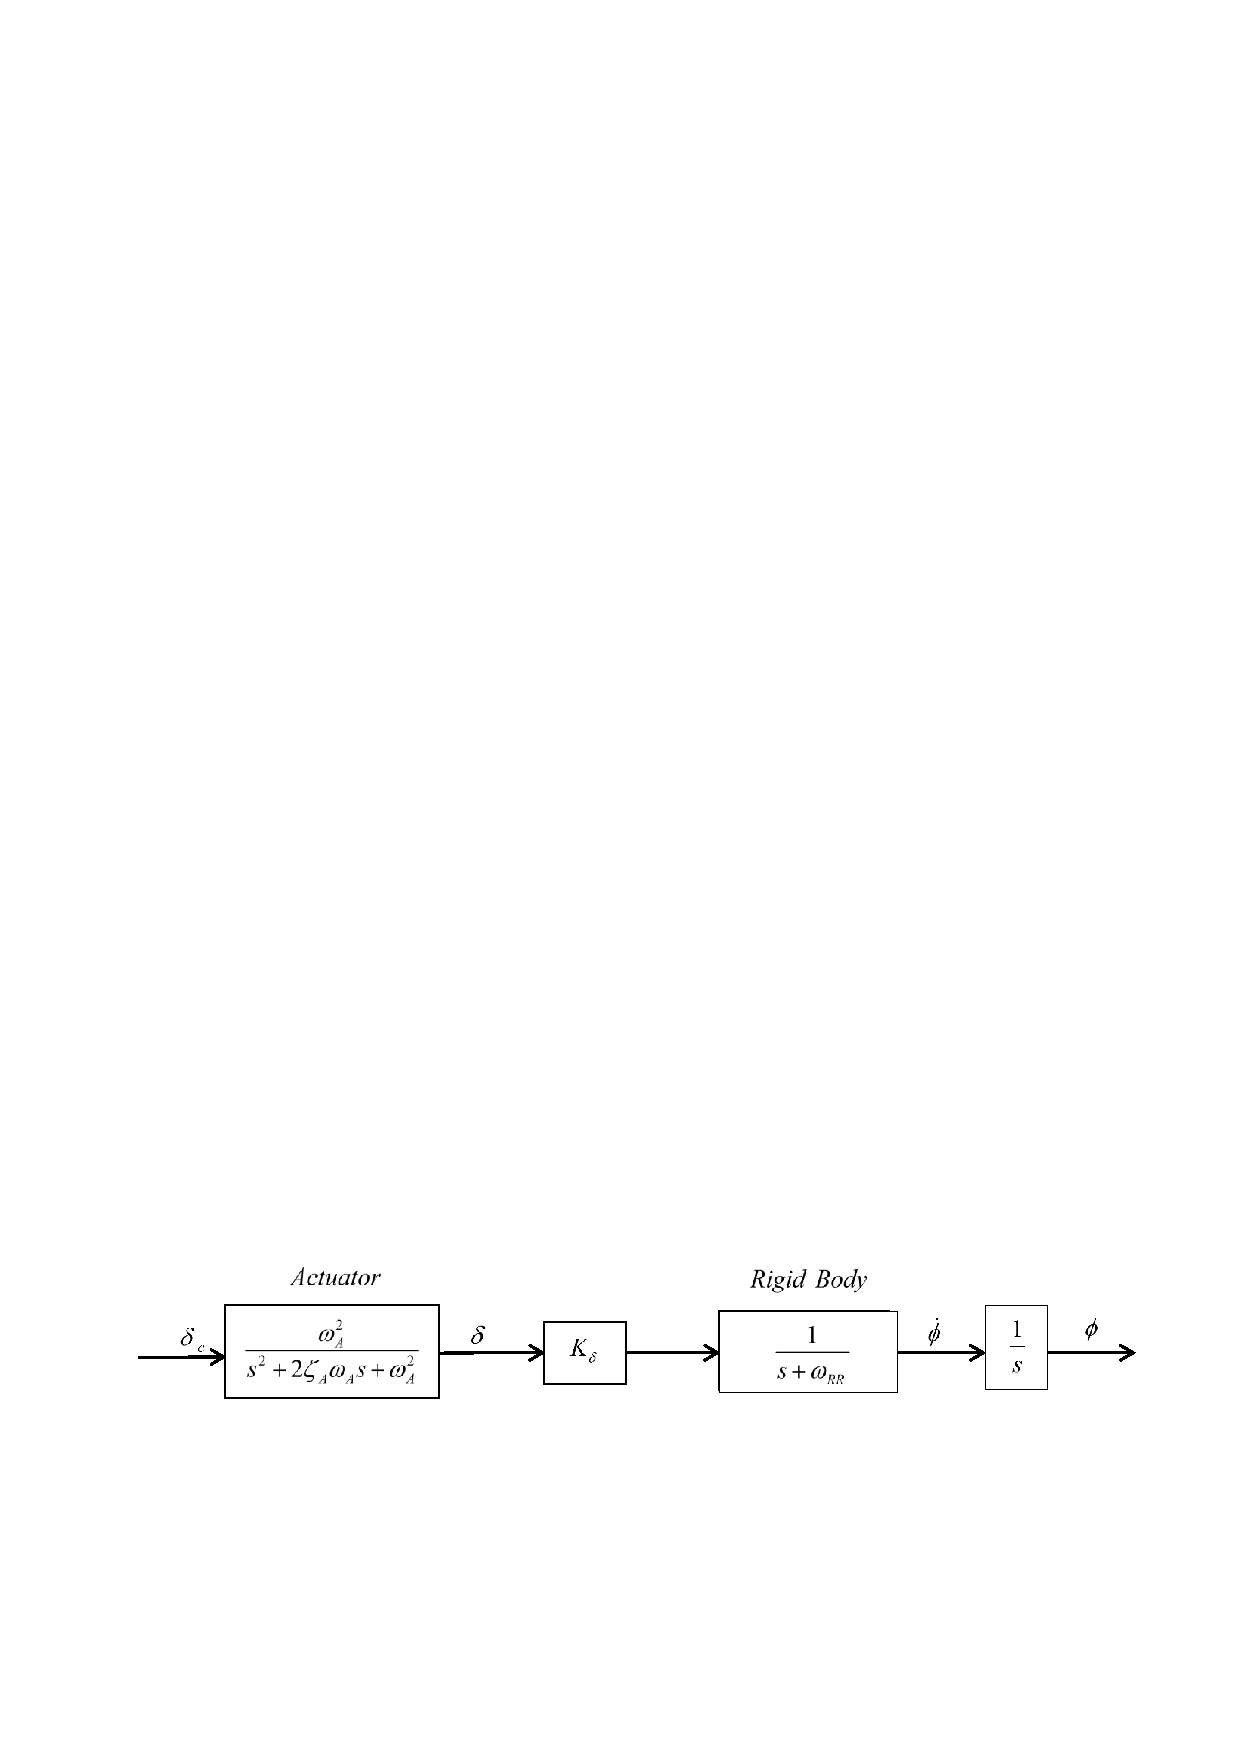
\includegraphics[width=0.8\linewidth]{fig4}
	\end{figure}
\end{frame}
%-------------------------------------------
\begin{frame}
\frametitle{Performance of UDE based controller with second order actuator in the loop}
\textbf{For simulation;}
\begin{itemize}  % Shows text in bullet point 		
		\item $\tau$ continues to be 0.01
		\item All other simulation parameters are as per Table.1
		%\item damping factor $\zeta = 0.8$
				%\begin{enumerate}
					%\item Using these values, feedback gains $m_1$ and $m_2$ were evaluated to be 
					%\item $m_1=42.45$, $m_2=771.13$ 
				%\end{enumerate}
		%\item external disturbance $d_{ext}= 200$ rad/$s^2$
		%\item desired roll orientation $=0$ deg
		%\item initial condition in $\phi= 10$ deg
		%\item all other values as referred from Table.1
\end{itemize}
\end{frame}
%where , respectively. Now simulations were carried out using the control law (\ref{eq11})  for the simulation parameters discussed before. It may be noted that the effects of actuator dynamics are not accounted in the UDE based control law. The simulation results are presented in Fig. 3.
%-------------------------------------------------------------------------------Figure 4-------------------------------------------------------------------
%
\begin{frame} 
\frametitle{Performance of UDE based controller with second order actuator in the loop}
%\textbf{Simulation Output}
%\begin{figure}[h]
%\begin{center}
	%%\begin{subfigure}
	%%\subfigure[Output Response]{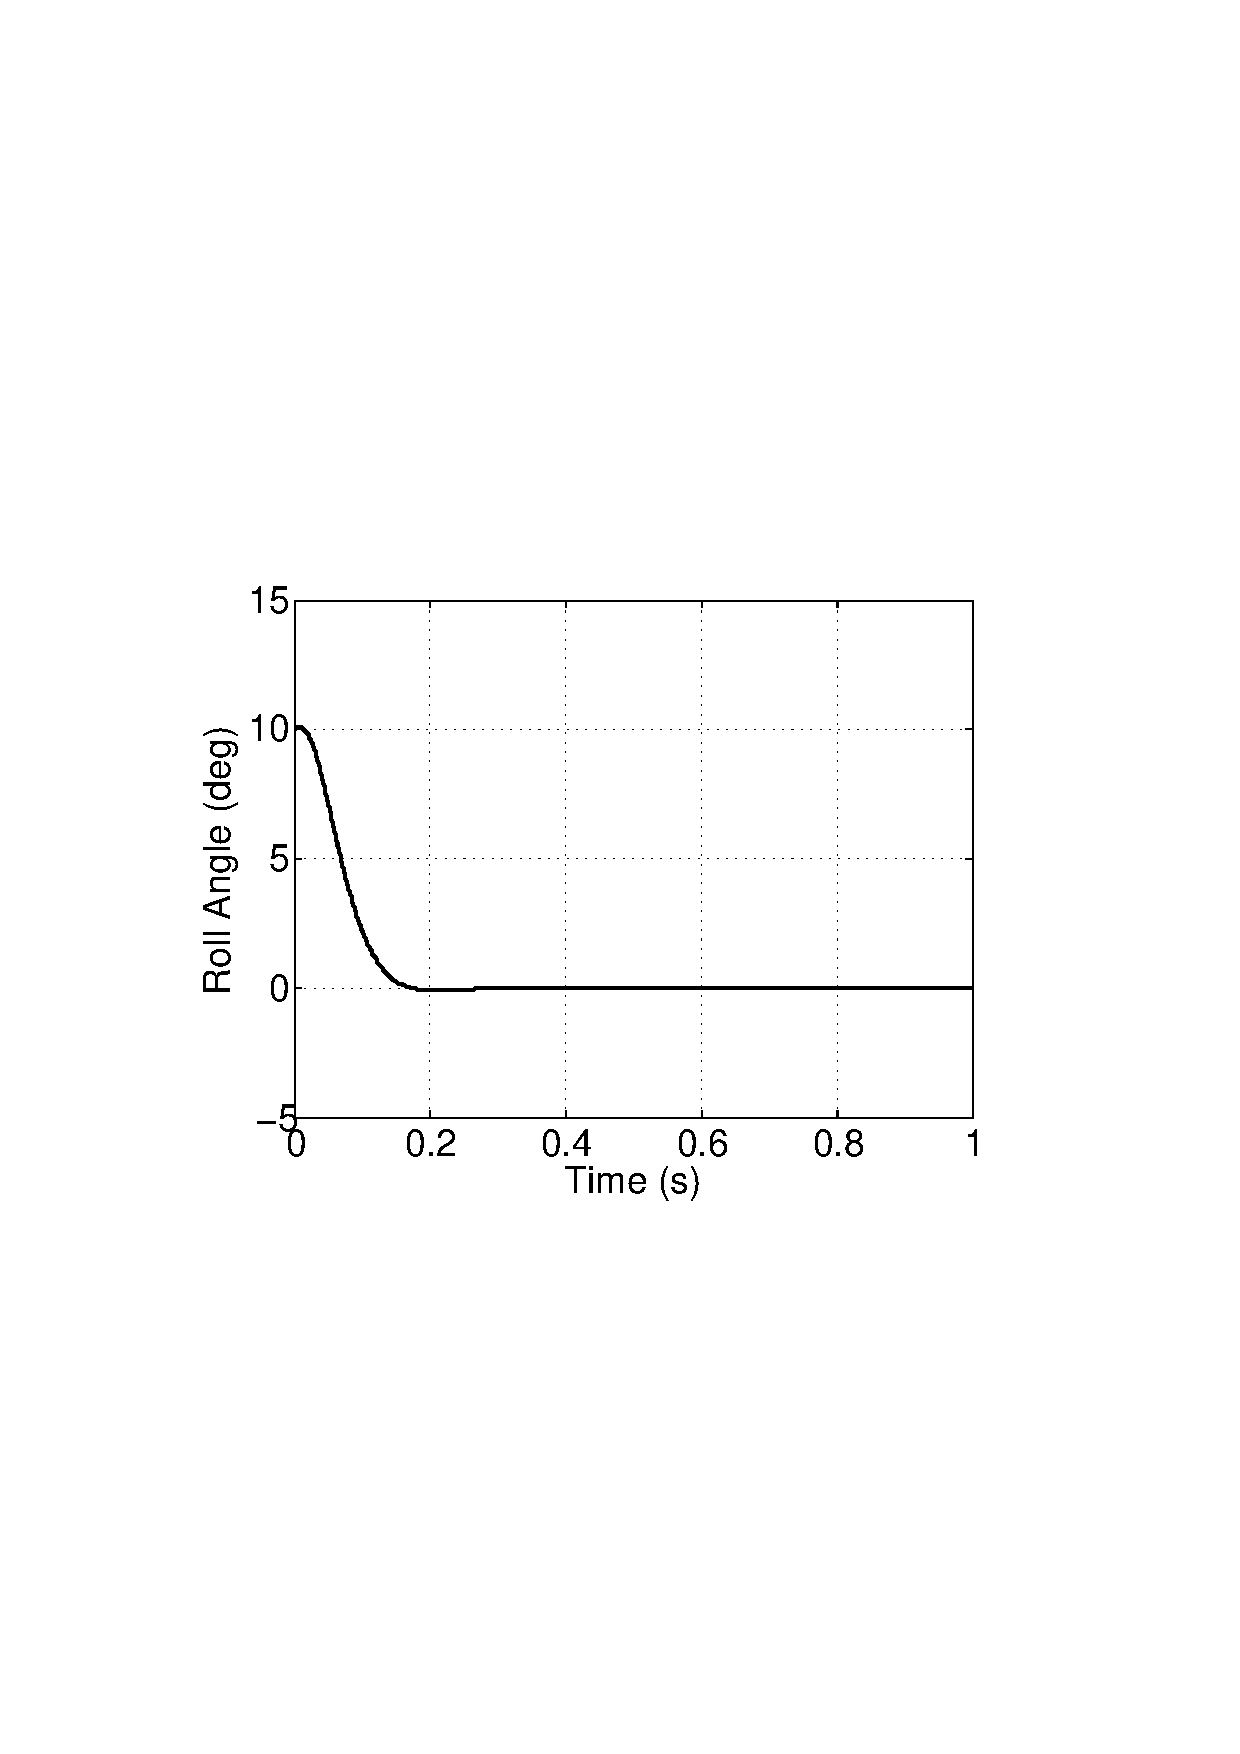
\includegraphics[width=8.4cm]{fig2a}}
	%{\includegraphics[width=4cm]{fig4a}}
	%%\subfigure[Output Response]{\includegraphics[width=4cm]{fig4a}}
	%%\includegraphics[width=8.4cm]{fig3a}    % The printed column width is 8.4 cm.
	%%\caption{Output response}
	%%\end{subfigure}
%%
	%%\begin{subfigure}
	%%\subfigure[Control Effort]{\includegraphics[width=4cm]{fig4b}}
	%%\includegraphics[width=8.4cm]{fig3b}    % The printed column width is 8.4 cm.
	%%\caption{Control Effort}
	%%\end{subfigure}
	%%\subfigure[Disturbance Estimation]{\includegraphics[width=4cm]{fig4c}}
	%\caption{Performance with UDE with second order actuator} 
%\label{fig4}
%\end{center}
%\end{figure}
%\includegraphics[width=3cm]{fig4a}
%%\caption{Output response}
%\includegraphics[width=3cm]{fig4b}
%\includegraphics[width=3cm]{fig4c}

\begin{figure}
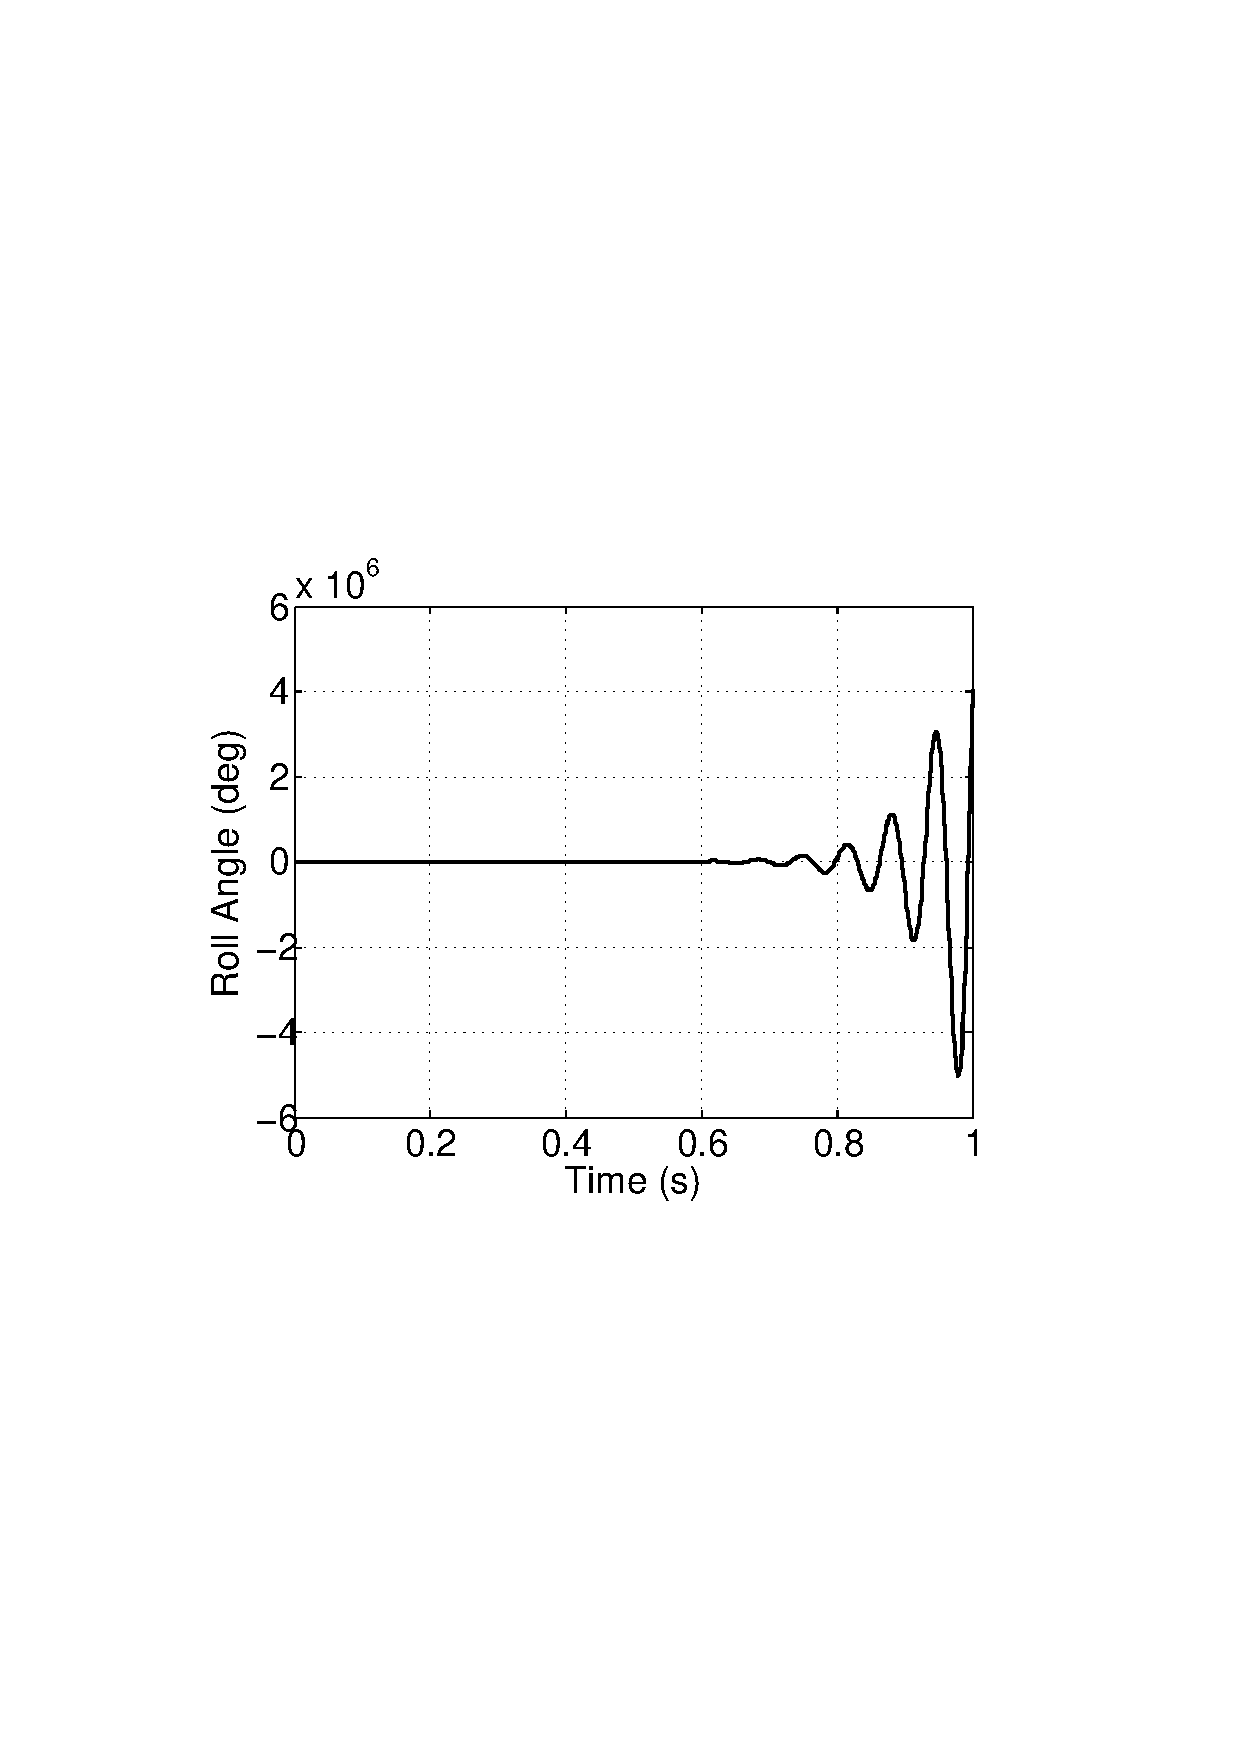
\includegraphics[width=3.7cm]{fig5a}
%\title{Output response}
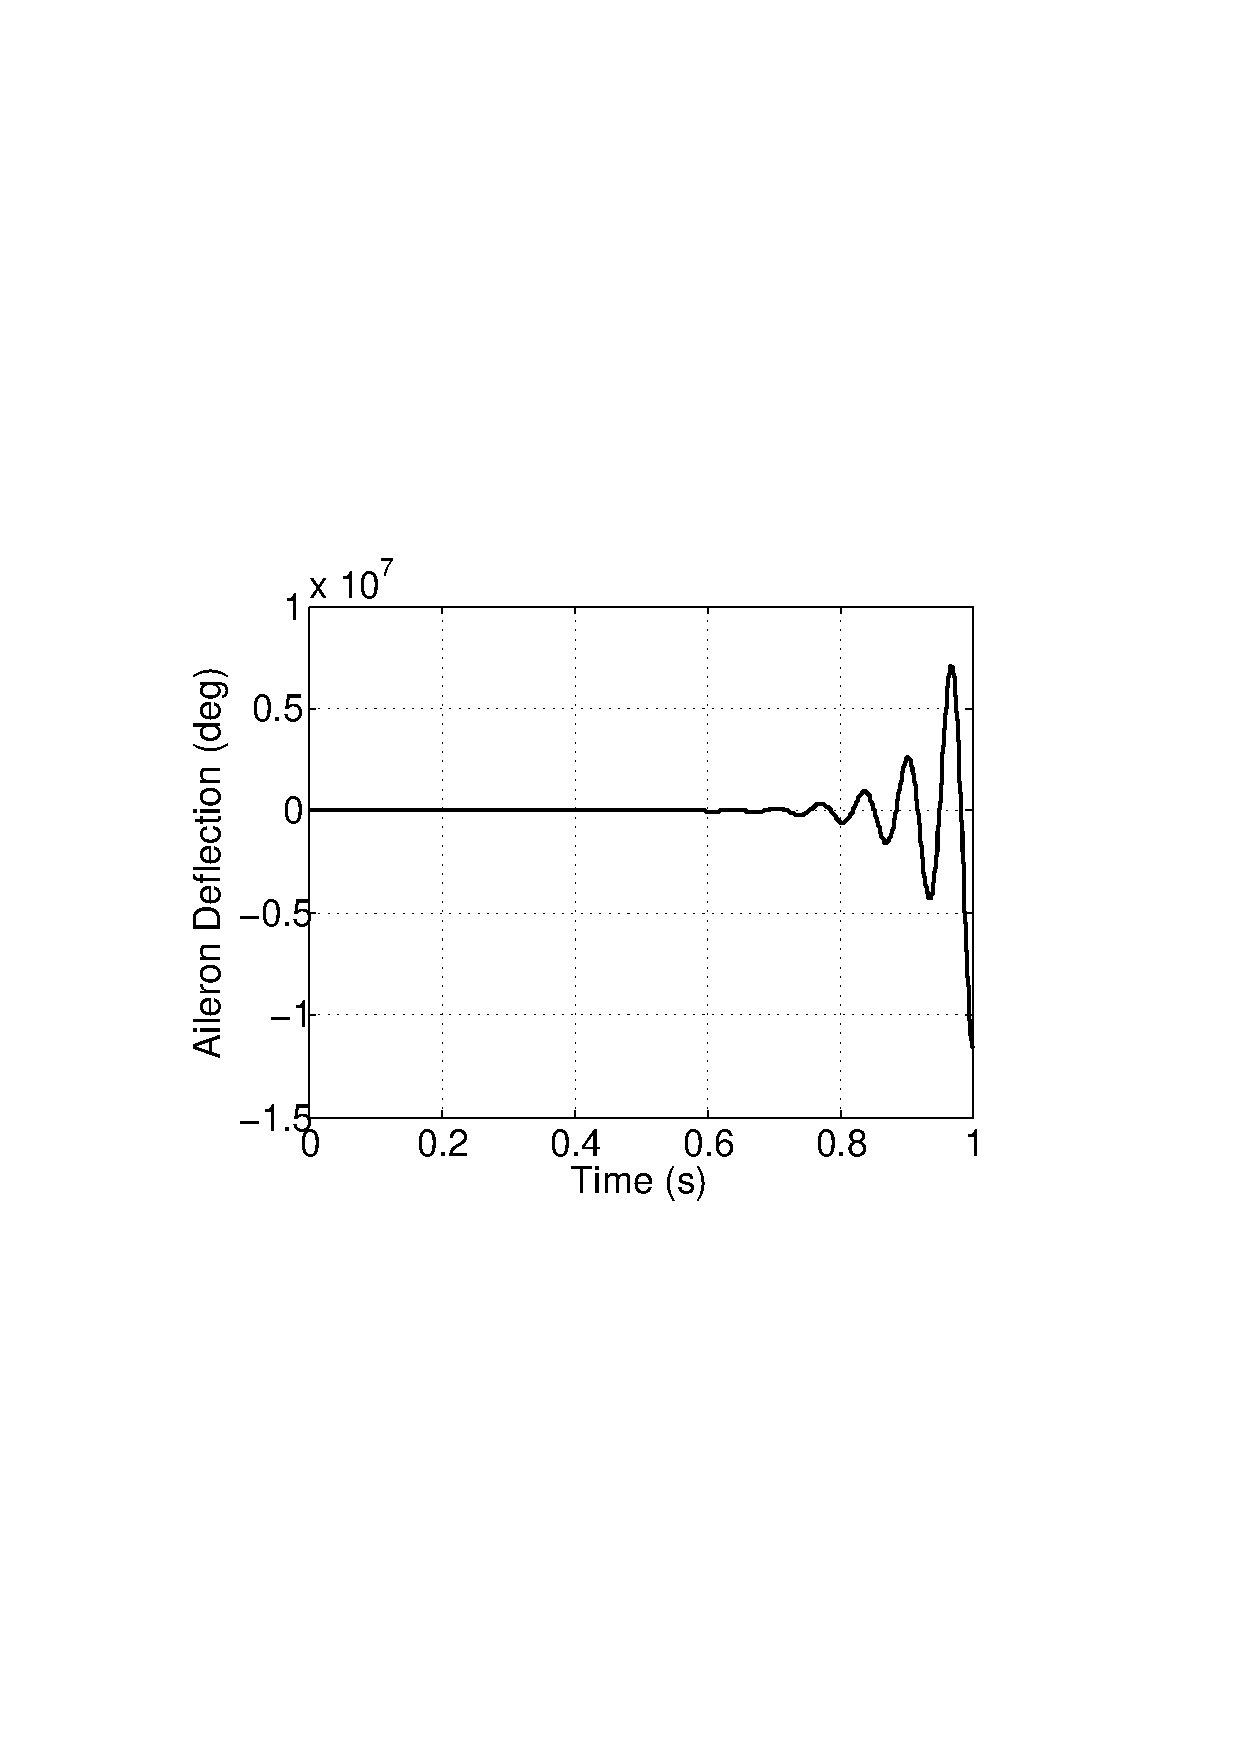
\includegraphics[width=3.7cm]{fig5b}
%\caption{Output response}
%\end{figure}
\begin{center}
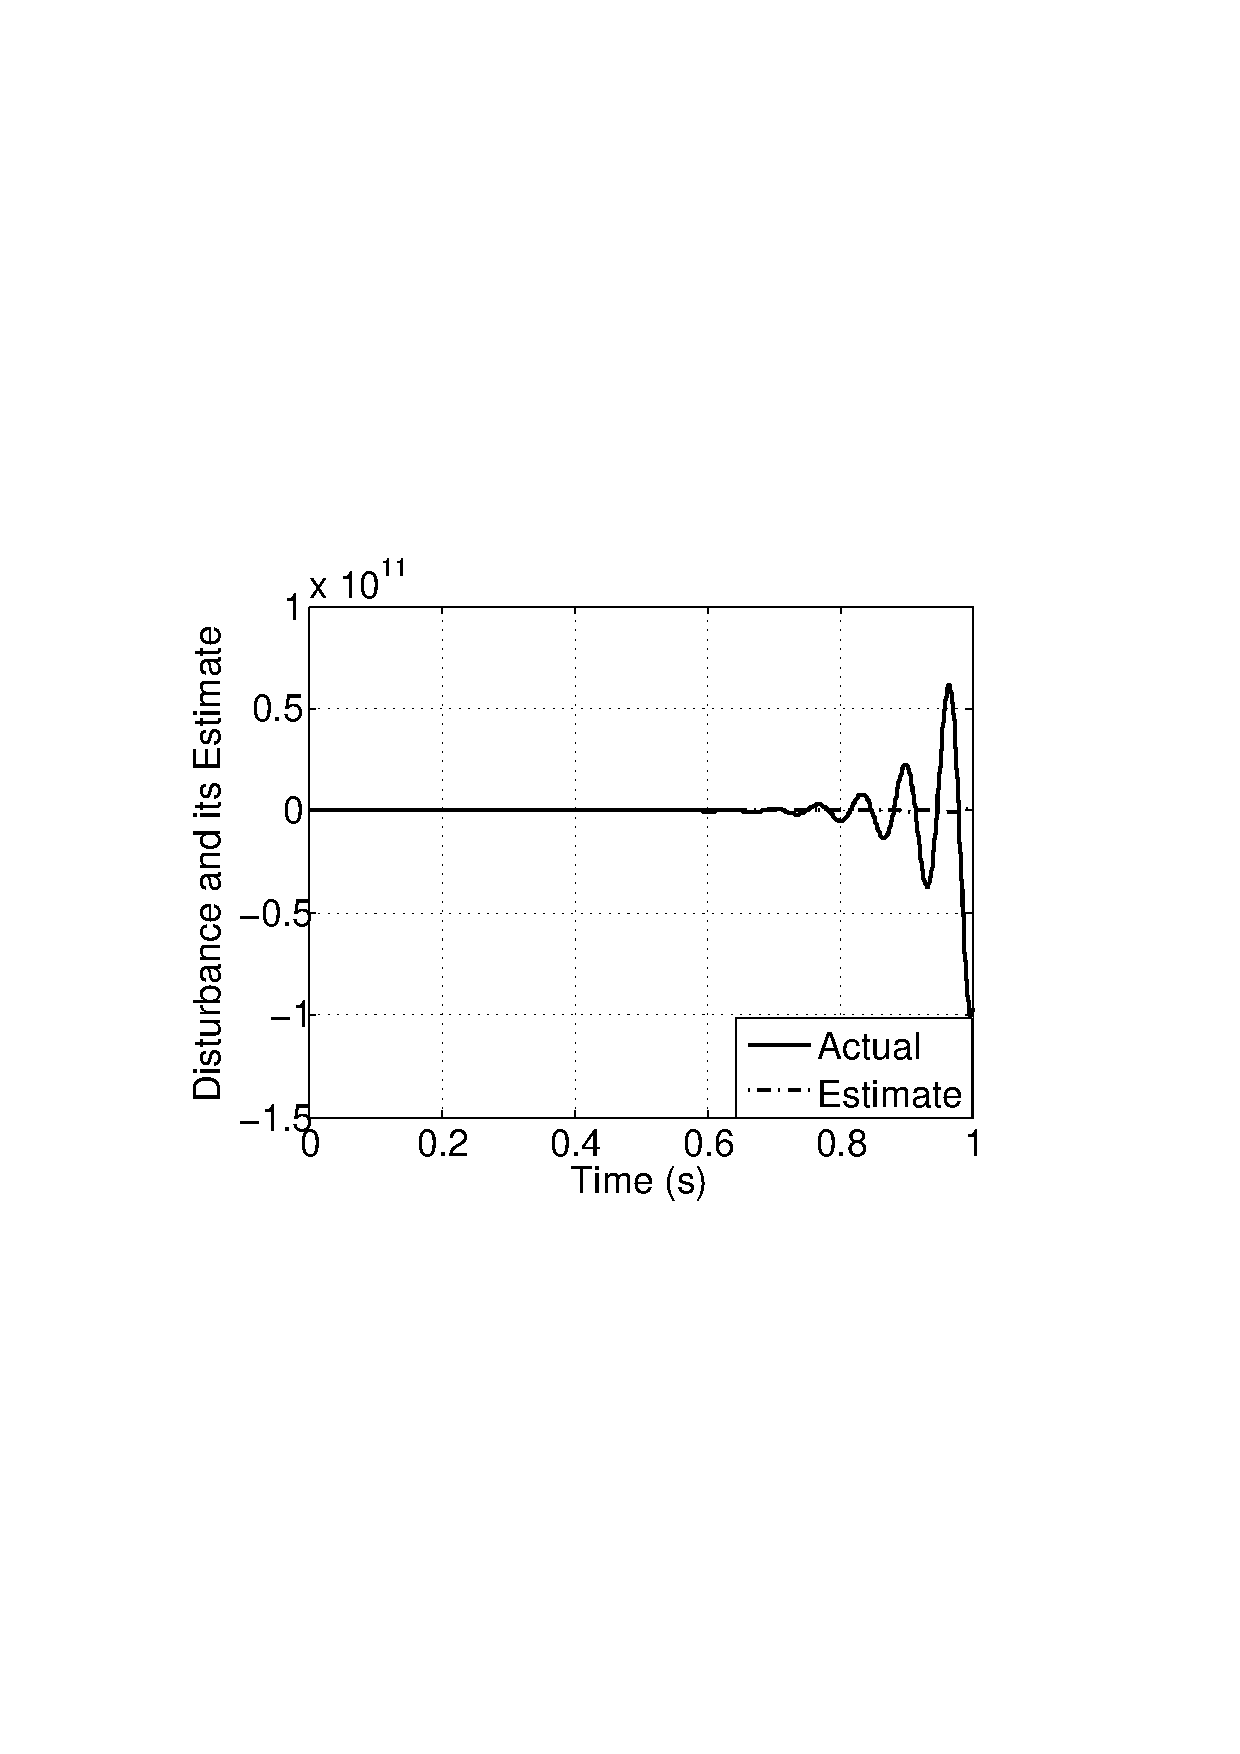
\includegraphics[width=3.7cm]{fig5c}
\end{center}
\end{figure}
\end{frame}
%-----------------------------------------------------------------------------------------------------------------------------------------
%---------------------------------------------------------------------
\section{Actuator compensated UDE based control law}
\begin{frame}
\frametitle{Actuator compensated UDE based control law}
\textbf{Need for actuator compensation}
\begin{itemize}  % Shows text in bullet point 	
	
		\item It has been observed that addition of a second order actuator in the plant, makes the system unstable
		\item There is a need to compensate the effects of the actuator by proper tuning the UDE based robust control law or by  designing a compensator for the actuator
		%\item For the combined fourth order system, availability of sensors to measure these variables cannot be guaranteed
		%\item This approach requires the availability of all the states for measurement and is used in the control law
		%\item Attempt must thus be made to avoid a fourth order plant
		%\item Taking $x_e = x_1 - x_{1ref}$
		%\begin{enumerate}
					%\item $\nu=-m_4x_e - m_3\dot{x}_e - m_2\ddot{x}_e - m_1\stackrel{\ldots}{x}_e$ 
					%\item $m_1$, $m_2$, $m_3$ and $m_4$ are feedback gains chosen for desired poles
					%\item By choosing the performance criterion as before, for this fourth order system, the desired poles are selected accordingly
				%\end{enumerate}
				
\end{itemize}
\end{frame}
%========================================================================================================================================
\subsection{Method 1: Tuning of $\tau$}
\begin{frame}
\frametitle{Method 1: Tuning of $\tau$}
Assuming uncertainties and disturbances in the original plant and expressing $\delta$ in terms of $\delta_c$,  we re-write the dynamics as
 %
%\begin{eqnarray}
%\dot{x}_1 &=& x_2 \nonumber \\
%\dot{x}_2 &=& - \omega_{RRn}x_2 + K_{\delta n}\delta + d
%\label{eq18}
%\end{eqnarray}
%
%Now, expressing $\delta$ in (\ref{eq18}) in terms of $\delta_c$ from (\ref{eq17}),;
 %
\begin{eqnarray*}
\dot{x}_1 &=& x_2 \nonumber \\
\dot{x}_2 &=& - \omega_{RRn}x_2 + {\color{red}{K_{\delta n}\left[\delta_c - {{1}\over{\omega^2_A}}\left( \ddot \delta + 2\zeta_A \omega_A \dot \delta\right)\right]}} \nonumber \\
&& + d
\label{eq19}
\end{eqnarray*}
\end{frame}
%---------------------------
\begin{frame}
\frametitle{Method 1: Tuning of $\tau$}
Since ${{-K_\delta n}\over{\omega^2_A}}\left( \ddot \delta + 2\zeta_A \omega_A \dot \delta\right)$ is unknown, it can be treated as an unknown disturbance and clubbed with $d$ and denoted as $d_1$
\begin{eqnarray*}
\dot{x}_1 &=& x_2 \nonumber \\
\dot{x}_2 &=& - \omega_{RRn}x_2 + K_{\delta n}\delta_c + d_1
\label{eq20}
\end{eqnarray*}
%
\begin{itemize}  % Shows text in bullet point 		
		\item $d_1 = {{-K_\delta n}\over{\omega^2_A}}\left( \ddot \delta + 2\zeta_A \omega_A \dot \delta\right) + d$
		\item $u_a =  \omega_{RRn
		}x_2$
		\item  $\nu = \ddot{\phi}_{ref} - m_1(\dot{\phi} - \dot{\phi}_{ref}) - m_2(\phi - \phi_{ref})$
		\item $u_d= - \frac{1}{\tau}\left[x_2 - \int \nu dt\right]$
		%\item Attempt must thus be made to avoid a fourth order plant
		%\item Taking $x_e = x_1 - x_{1ref}$
		%\begin{enumerate}
					%\item $\nu=-m_4x_e - m_3\dot{x}_e - m_2\ddot{x}_e - m_1\stackrel{\ldots}{x}_e$ 
					%\item $m_1$, $m_2$, $m_3$ and $m_4$ are feedback gains chosen for desired poles
					%\item By choosing the performance criterion as before, for this fourth order system, the desired poles are selected accordingly
				%\end{enumerate}
				
\end{itemize}
\end{frame}
%%with $d_1 = {{-K_\delta n}\over{\omega^2_A}}\left( \ddot \delta + 2\zeta_A \omega_A \dot \delta\right) + d$.
%%For this system (\ref{eq20}), the control law (\ref{eq5})  and its components are defined as $u_a =  \omega_{RR}x_2$, $\nu = \ddot{\phi}_{ref} - m_1(\dot{\phi} - \dot{\phi}_{ref}) - m_2(\phi - \phi_{ref})$ and $u_d= - \frac{1}{\tau}\left[x_2 - \int \nu dt\right]$. As before the feedback gains $m_1$ and $m_2$ are same as in Section I. It may be noted that unlike the previous discussions, the control term $u_d$ caters for an additional unknown term ${{-K_\delta n}\over{\omega^2_A}}\left( \ddot \delta + 2\zeta_A \omega_A \dot \delta\right)$ in addition to $d$. This calls for careful choice of $\tau$ to take care of $d_1$. Since the stability analysis for the UDE based control law for similar systems is available in the literature, it has been omitted.
%%------------------------------------------------------------------------------------------------------------------------------------------------------
%\subsection{ of UDE controller with actuator compensation}
%\subsubsection{Performance of UDE based control law with actuator compensation using Method 1}
\begin{frame}
\frametitle{Performance of UDE based control law with actuator compensation using Method 1}
Simulations were carried out with the data in Table 1, with the value of filter constant $ \tau$ chosen as follows;
\begin{itemize}  % Shows text in bullet point 		
		\item $\tau$ when chosen to be 0.01 rendered the system unstable
		\item It was thus varied to achieve the desired performance
		\item As the value of $\tau$ increases from 0.01 till 0.025, the system remained unstable
		\item On further increasing the value of $\tau$, the system gradually began to stabilize
		\item The value of $\tau$ was thereby tuned to achieve the best possible performance
\end{itemize}

\textbf{The value of $\tau$ which gave the best possible performance was 0.04 }
\end{frame}
%%Simulations were carried out with the data given in Table 1. The time constant $\tau$ when chosen to be 0. 01 rendered the system unstable. Hence it was varied to achieve the desired performance. It was observed that as the value of $\tau$ increases from 0. 01 till 0. 025, the system remained unstable, similar to the performance in Fig. 3. On further increasing the value of $\tau$, the system gradually began to stabilize. Thus, the value of $\tau$ was tuned to achieve the best possible performance; results of which is shown in Fig. 5 for $\tau = 0.04$.
%%-------------------------------------------------------------------------------------------------------------------Figure 6----------------------------------------------------------------------------------------------
%%

\begin{frame}
\frametitle{Performance of UDE based control law with actuator compensation using Method 1}
%\textbf{Simulation Output}
%%\begin{figure}[h]

	%%\begin{subfigure}
	%%\subfigure[Control Effort]{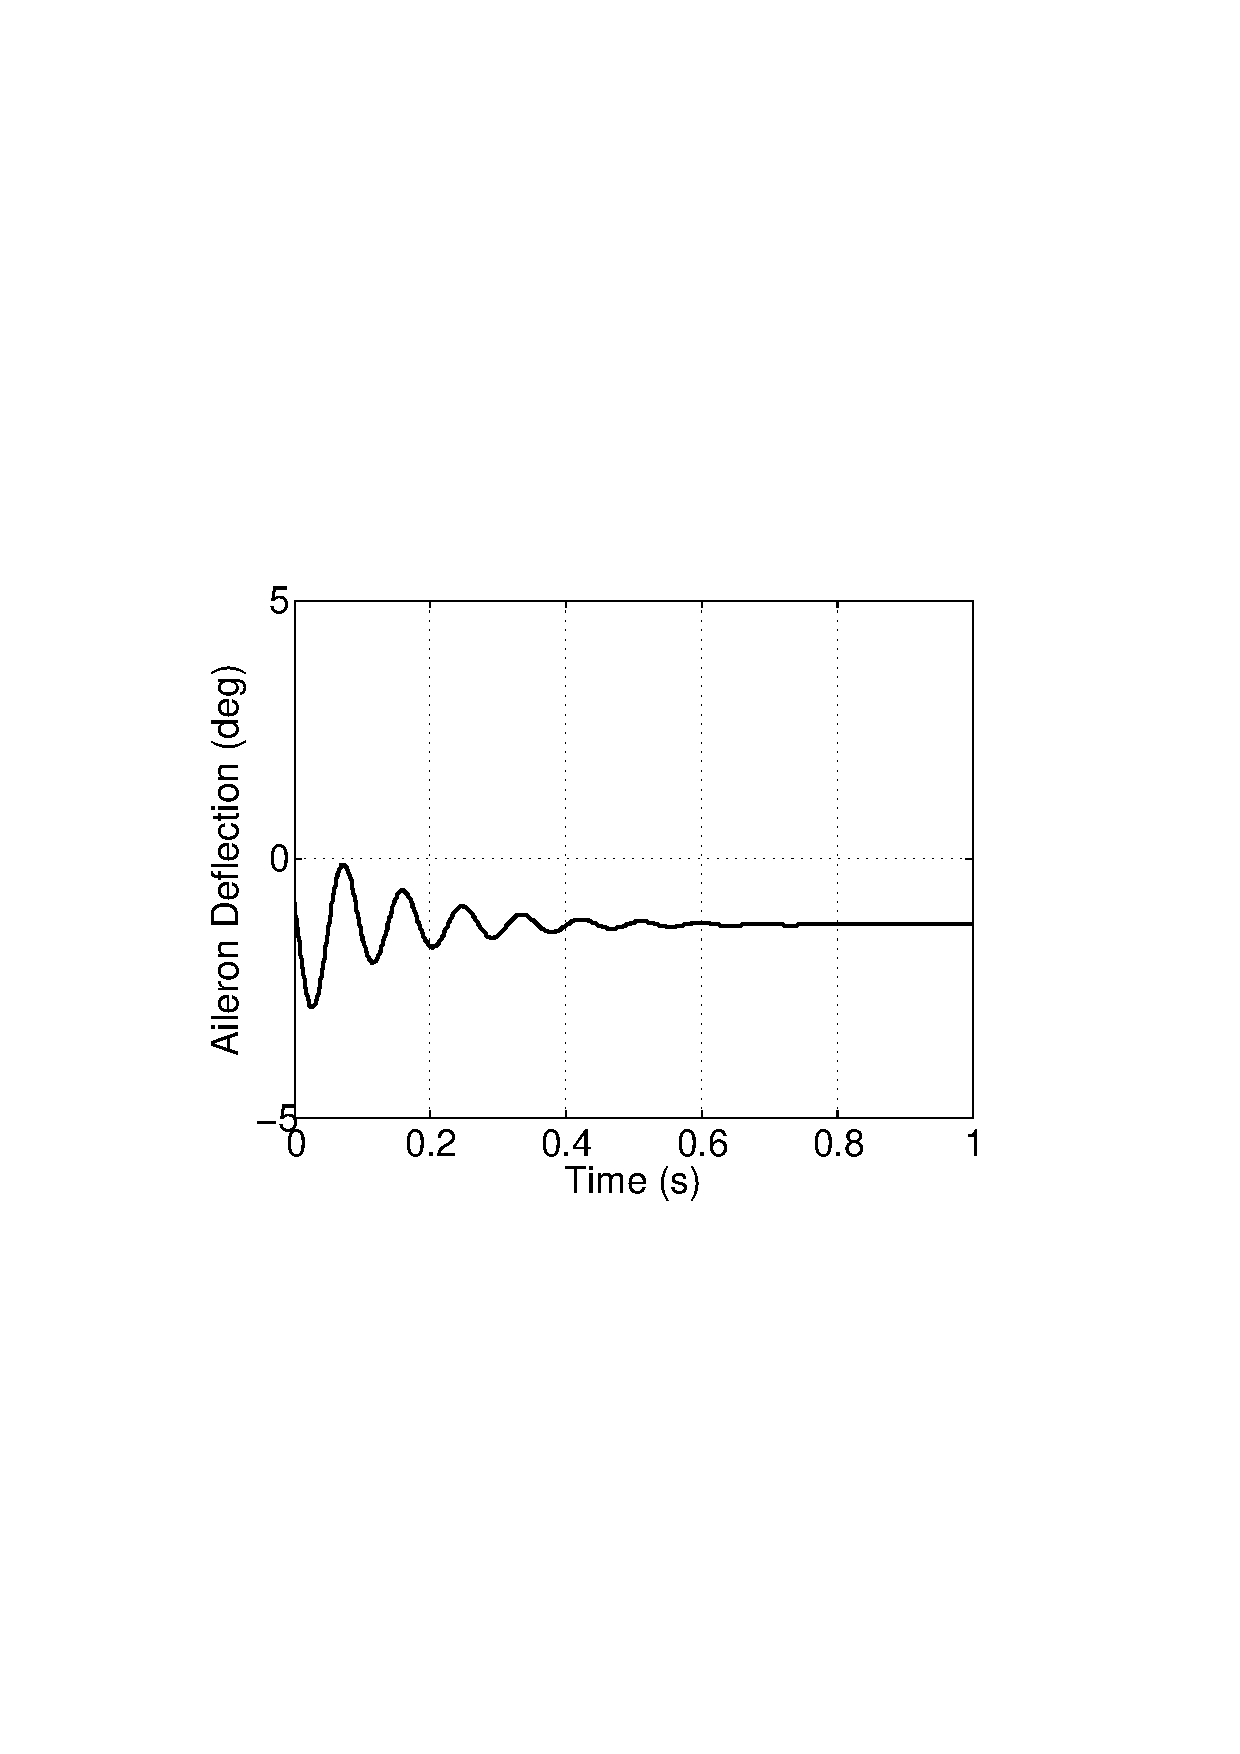
\includegraphics[width=4cm]{fig6b}}
	%%\includegraphics[width=8.4cm]{fig3b}    % The printed column width is 8.4 cm.
	%%\caption{Control Effort}
	%%\end{subfigure}
	%%\subfigure[Disturbance Estimation]{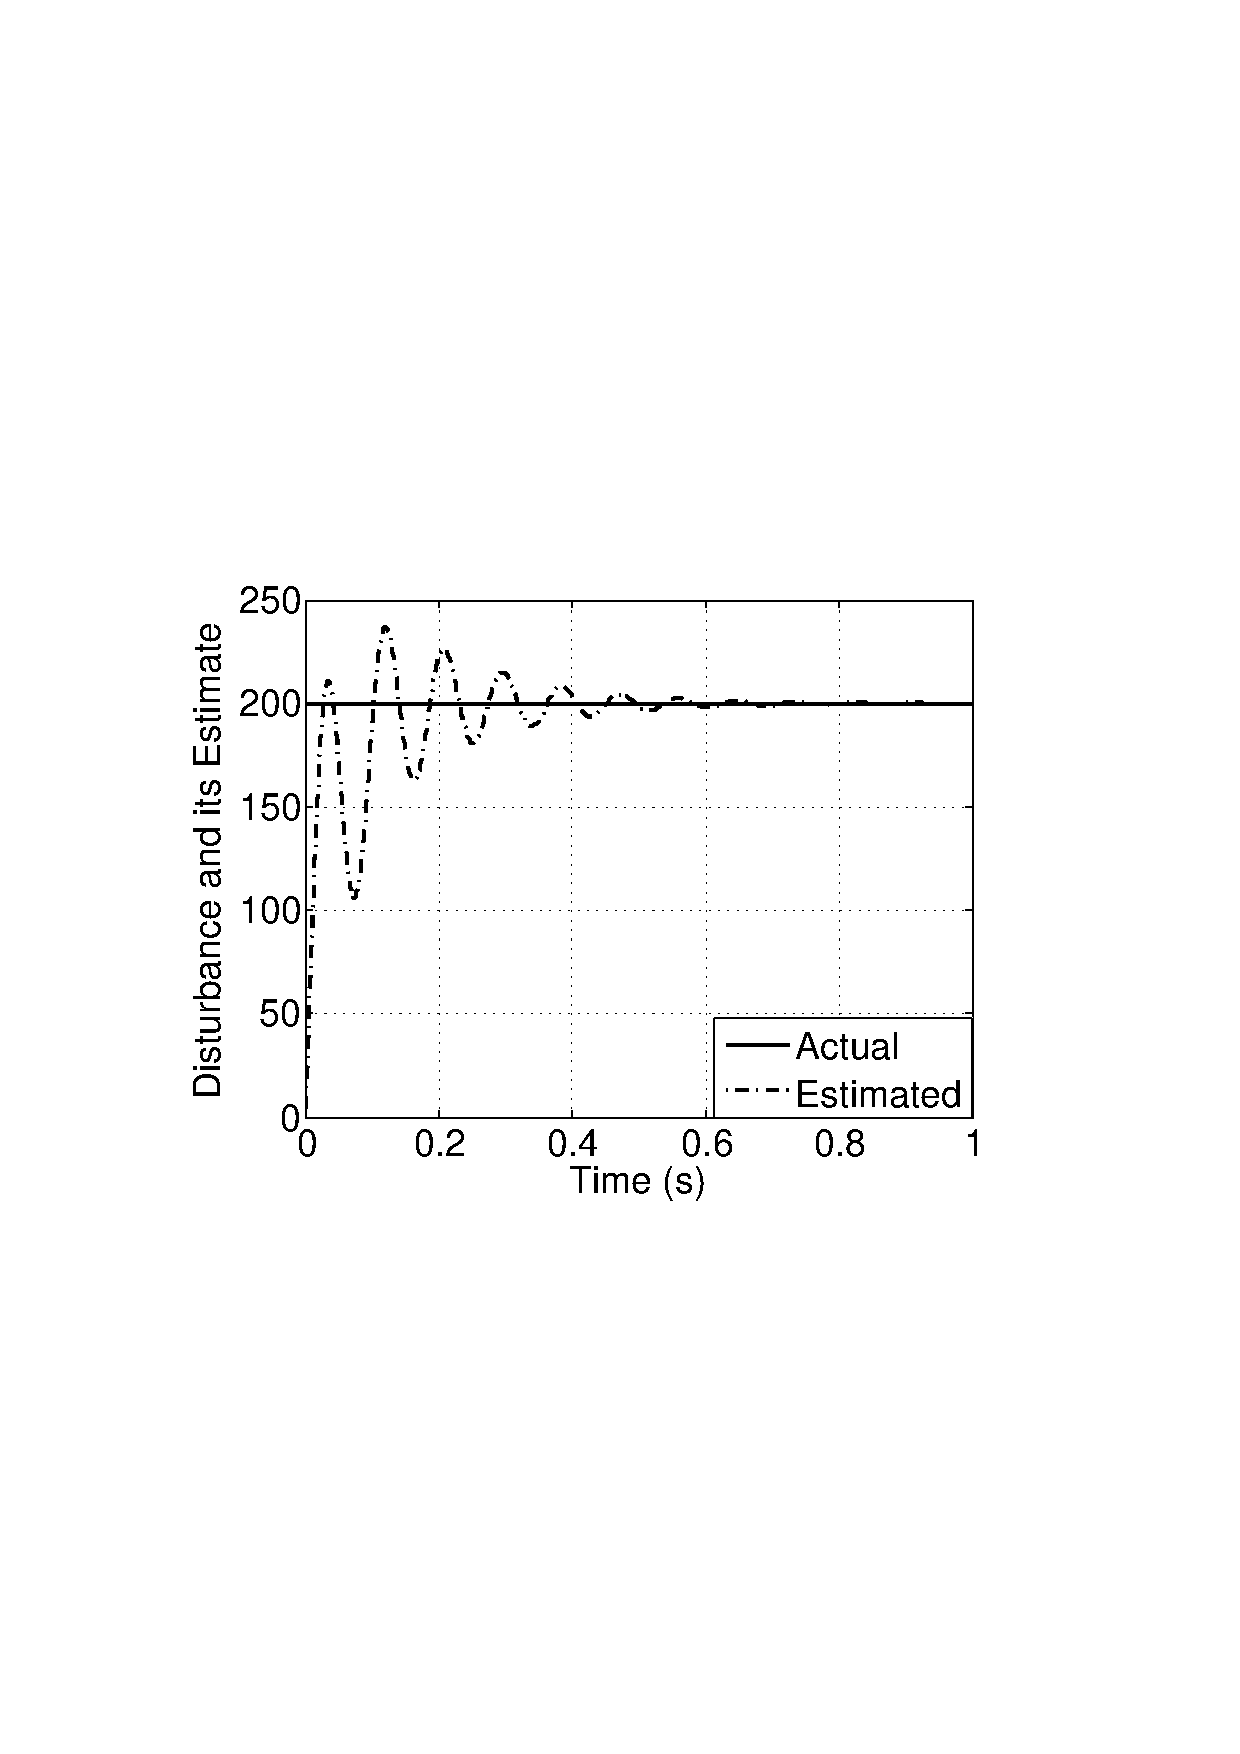
\includegraphics[width=4cm]{fig6c}}
	%%\caption{Performance with UDE with actuator compensation} 
%%\label{fig6}
%%\end{center}
%%\end{figure}
%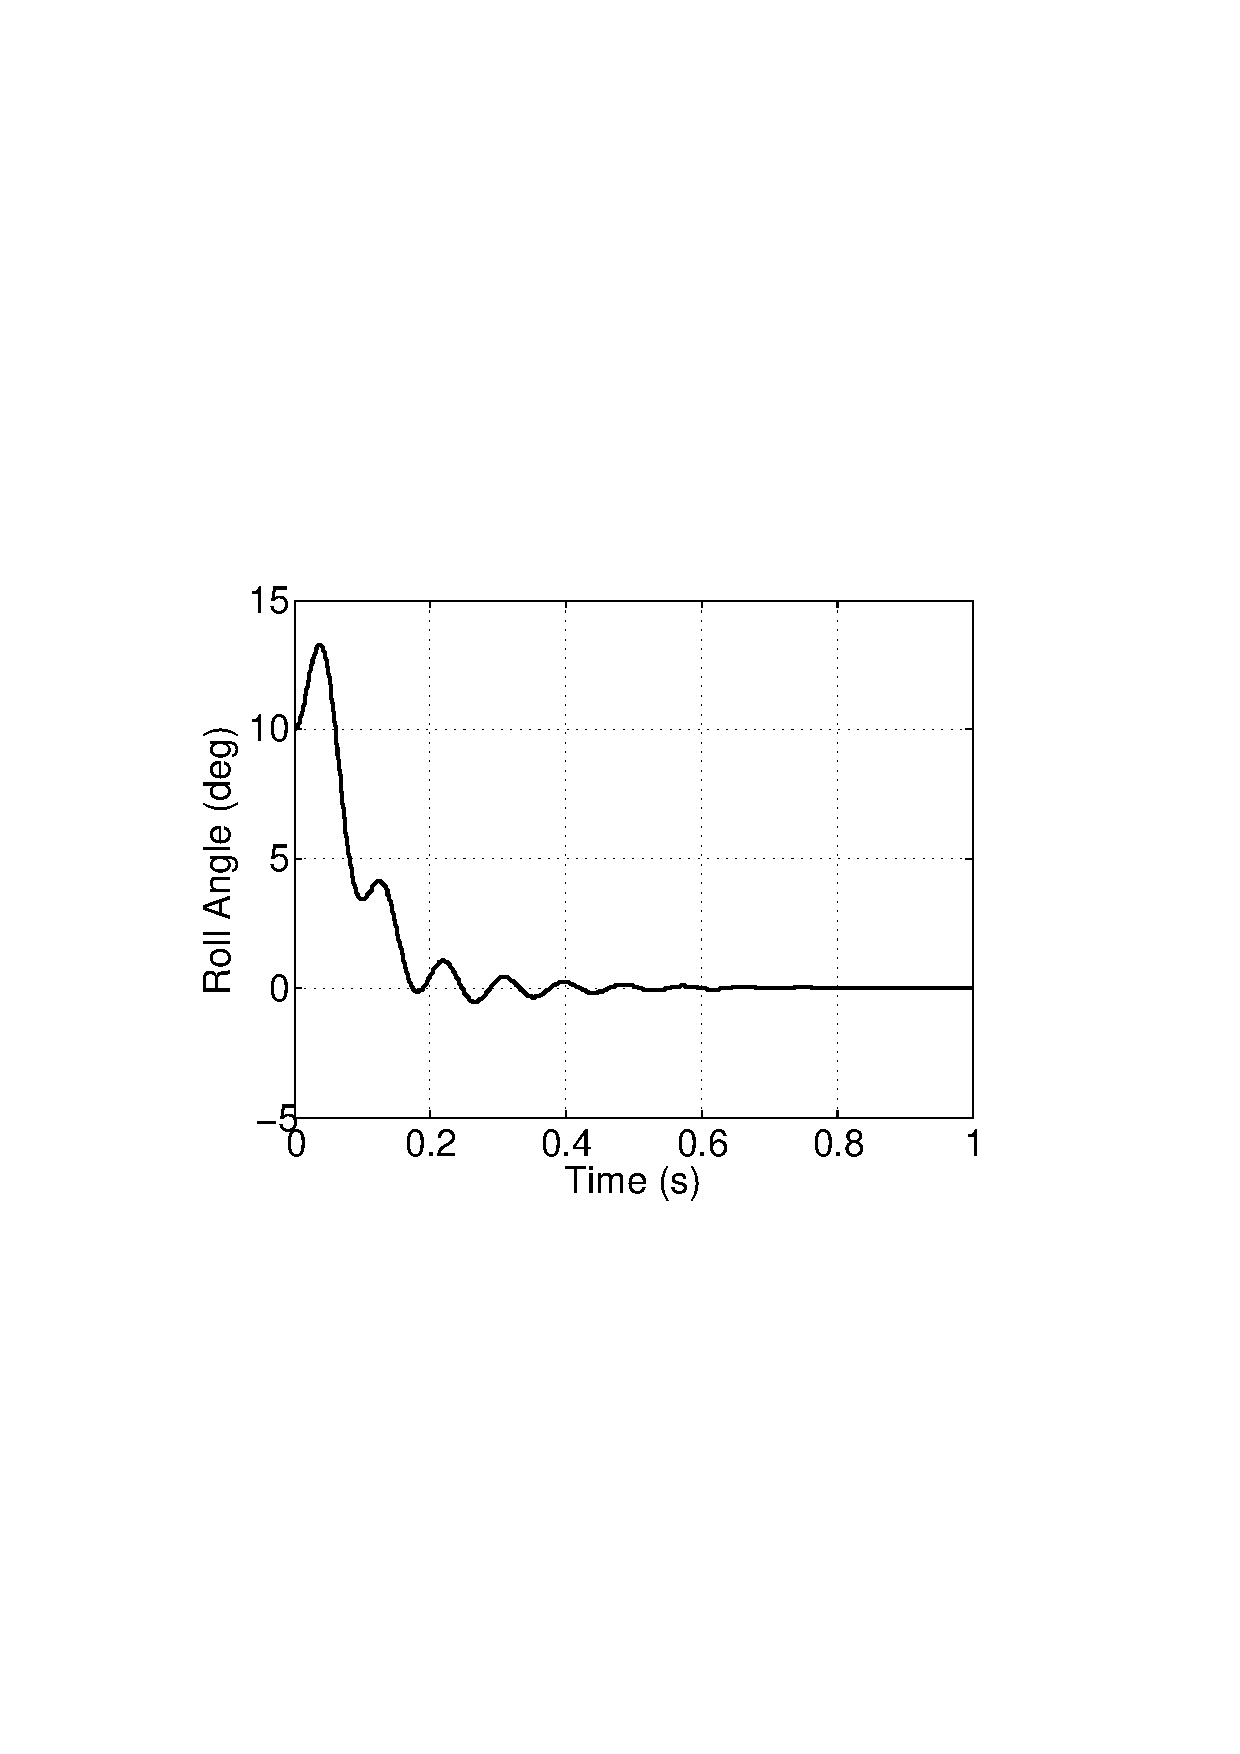
\includegraphics[width=3cm]{fig6a}
%%\caption{Output response}
%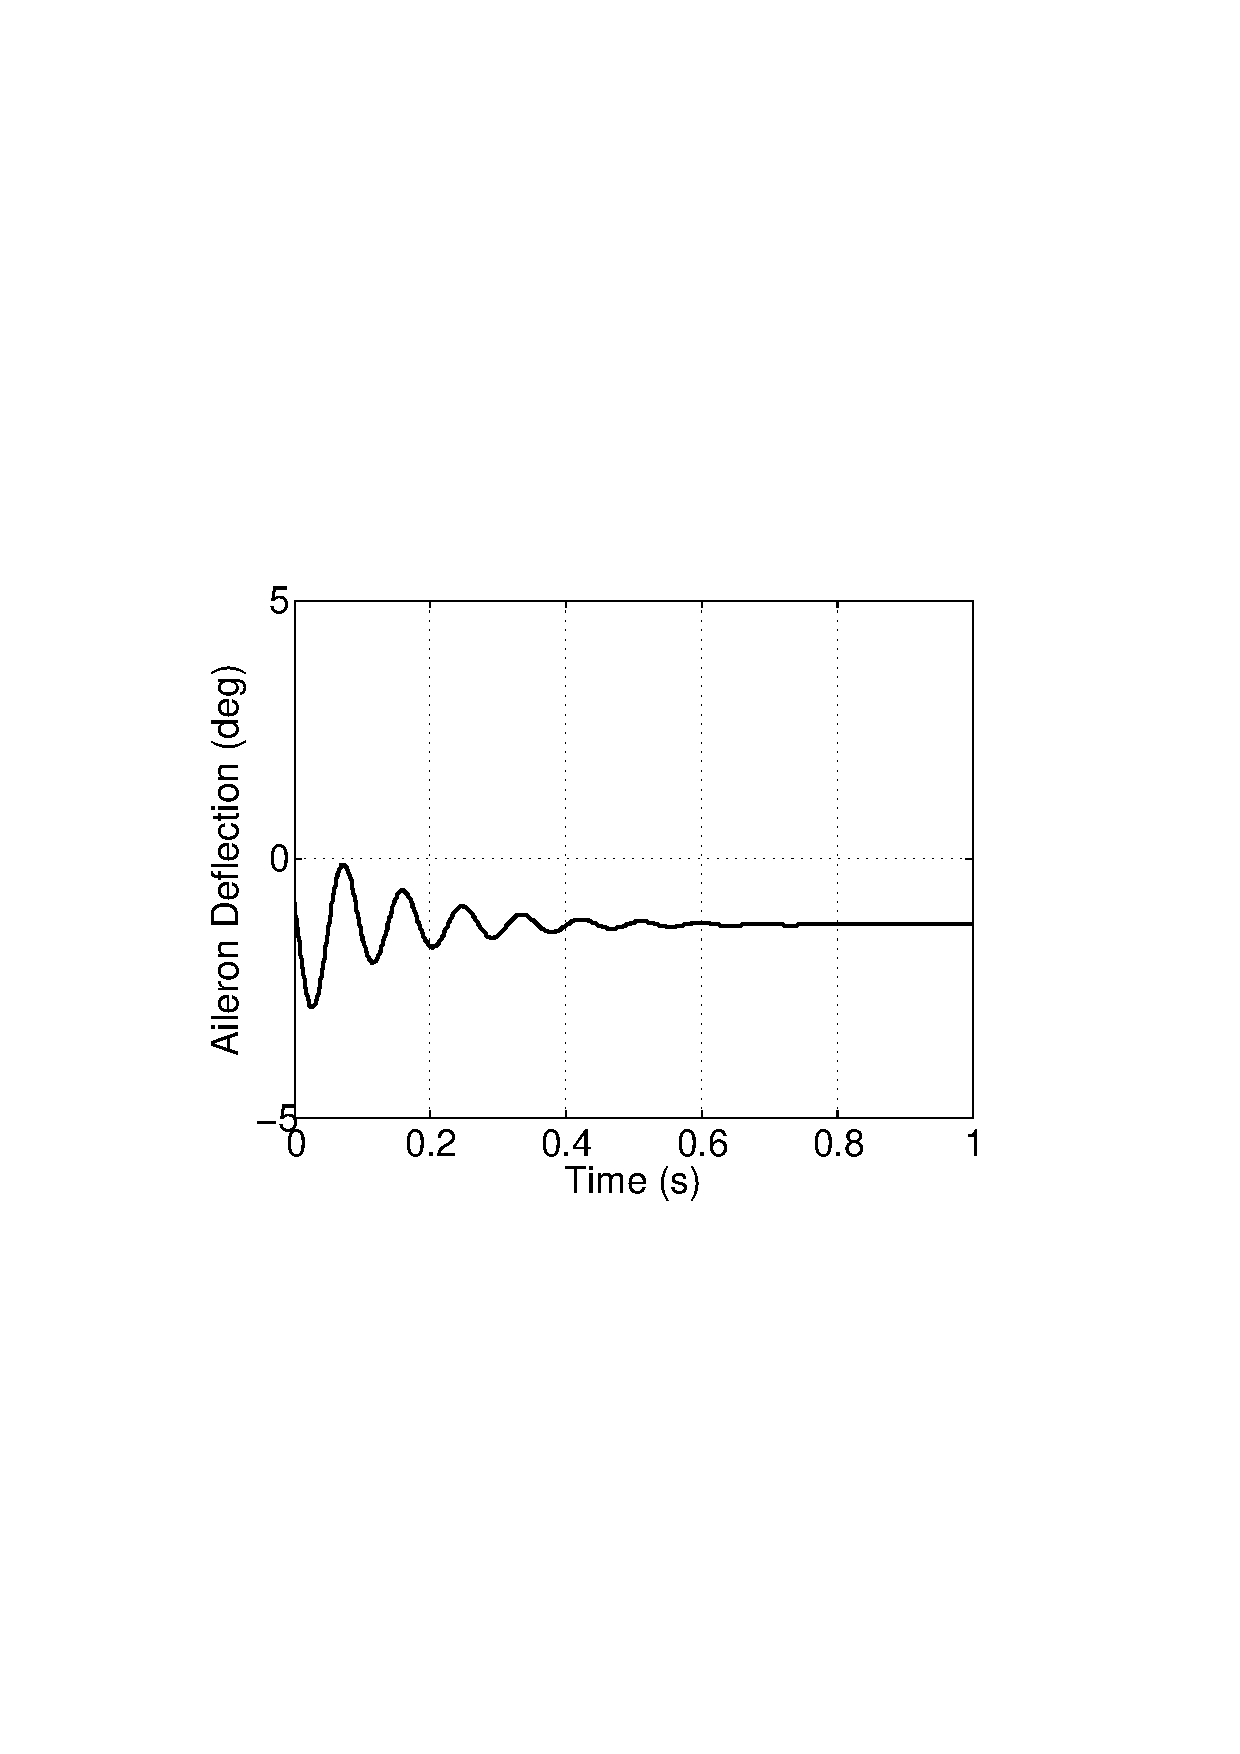
\includegraphics[width=3cm]{fig6b}
%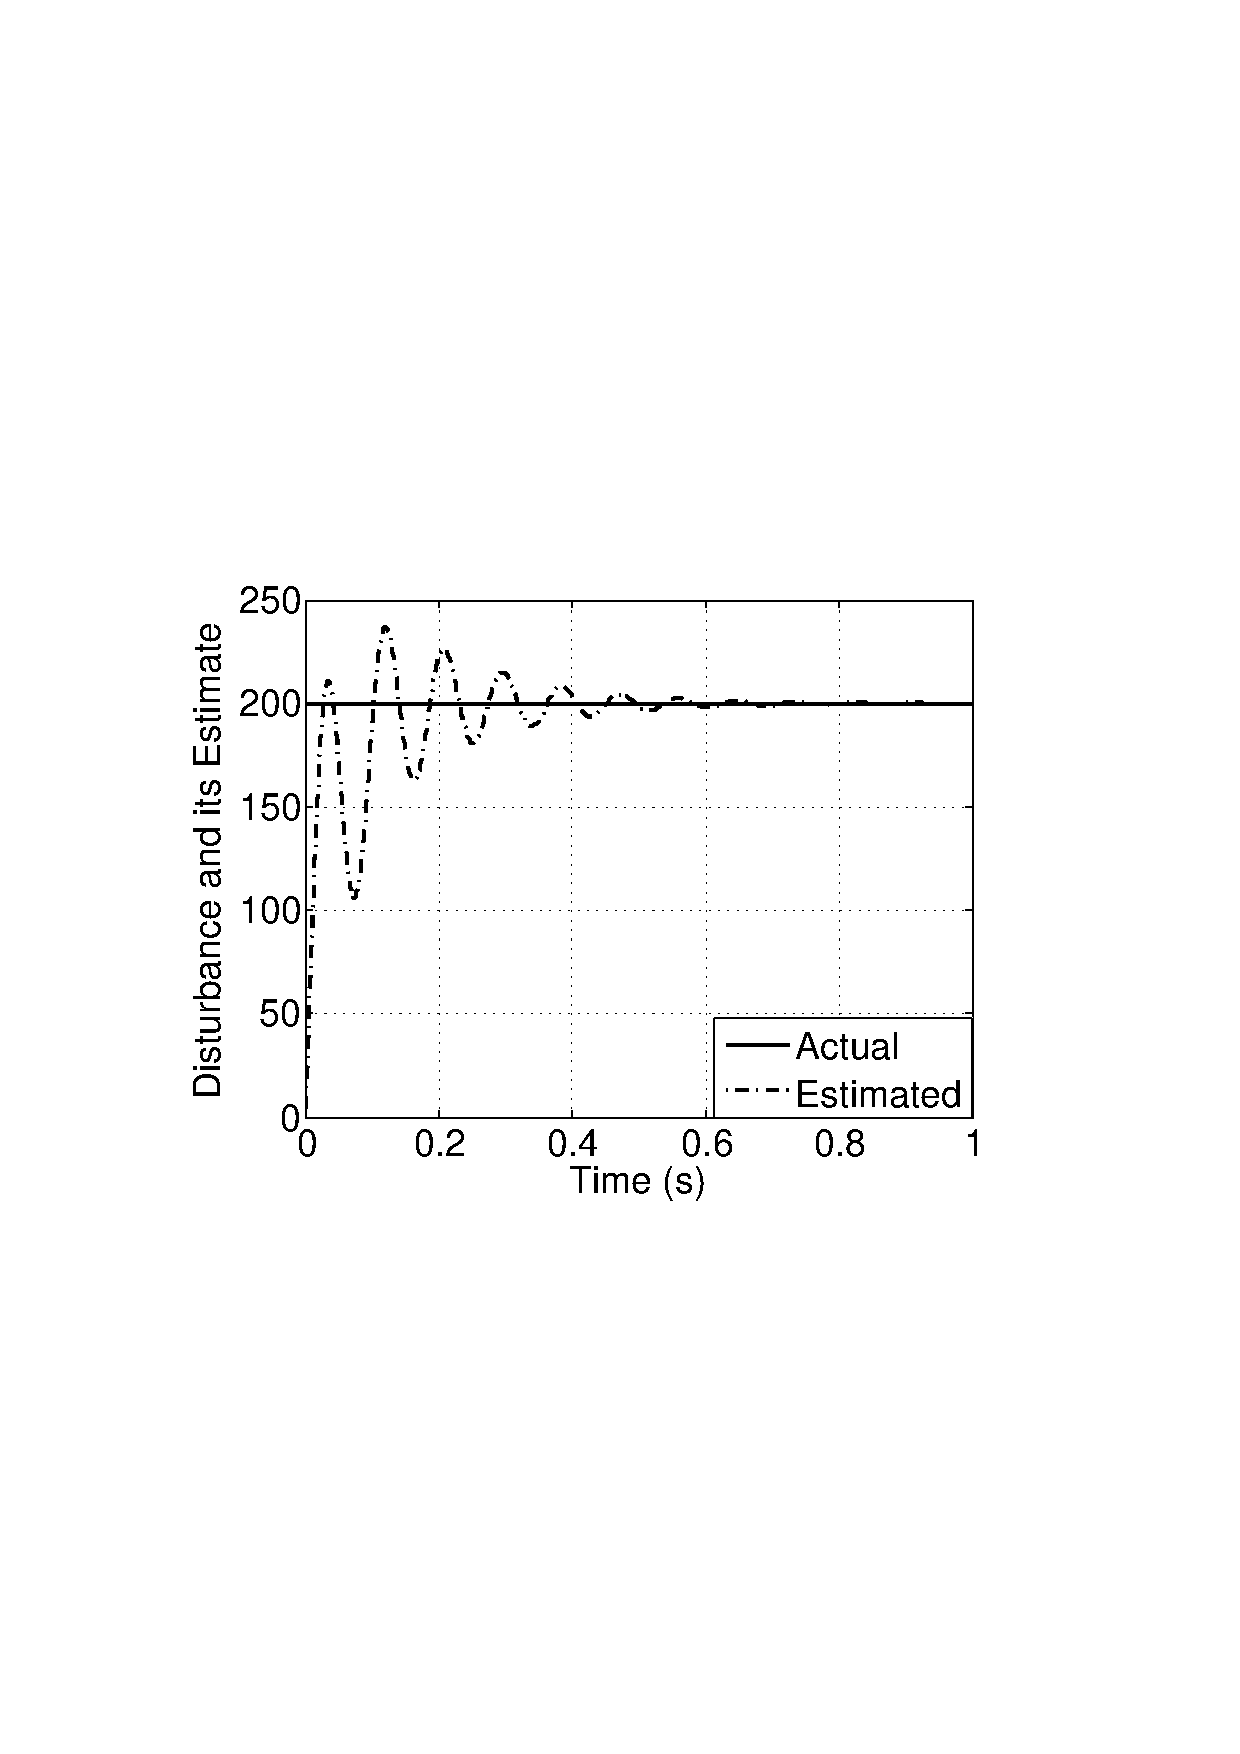
\includegraphics[width=3cm]{fig6c}
%change size here
\begin{figure}
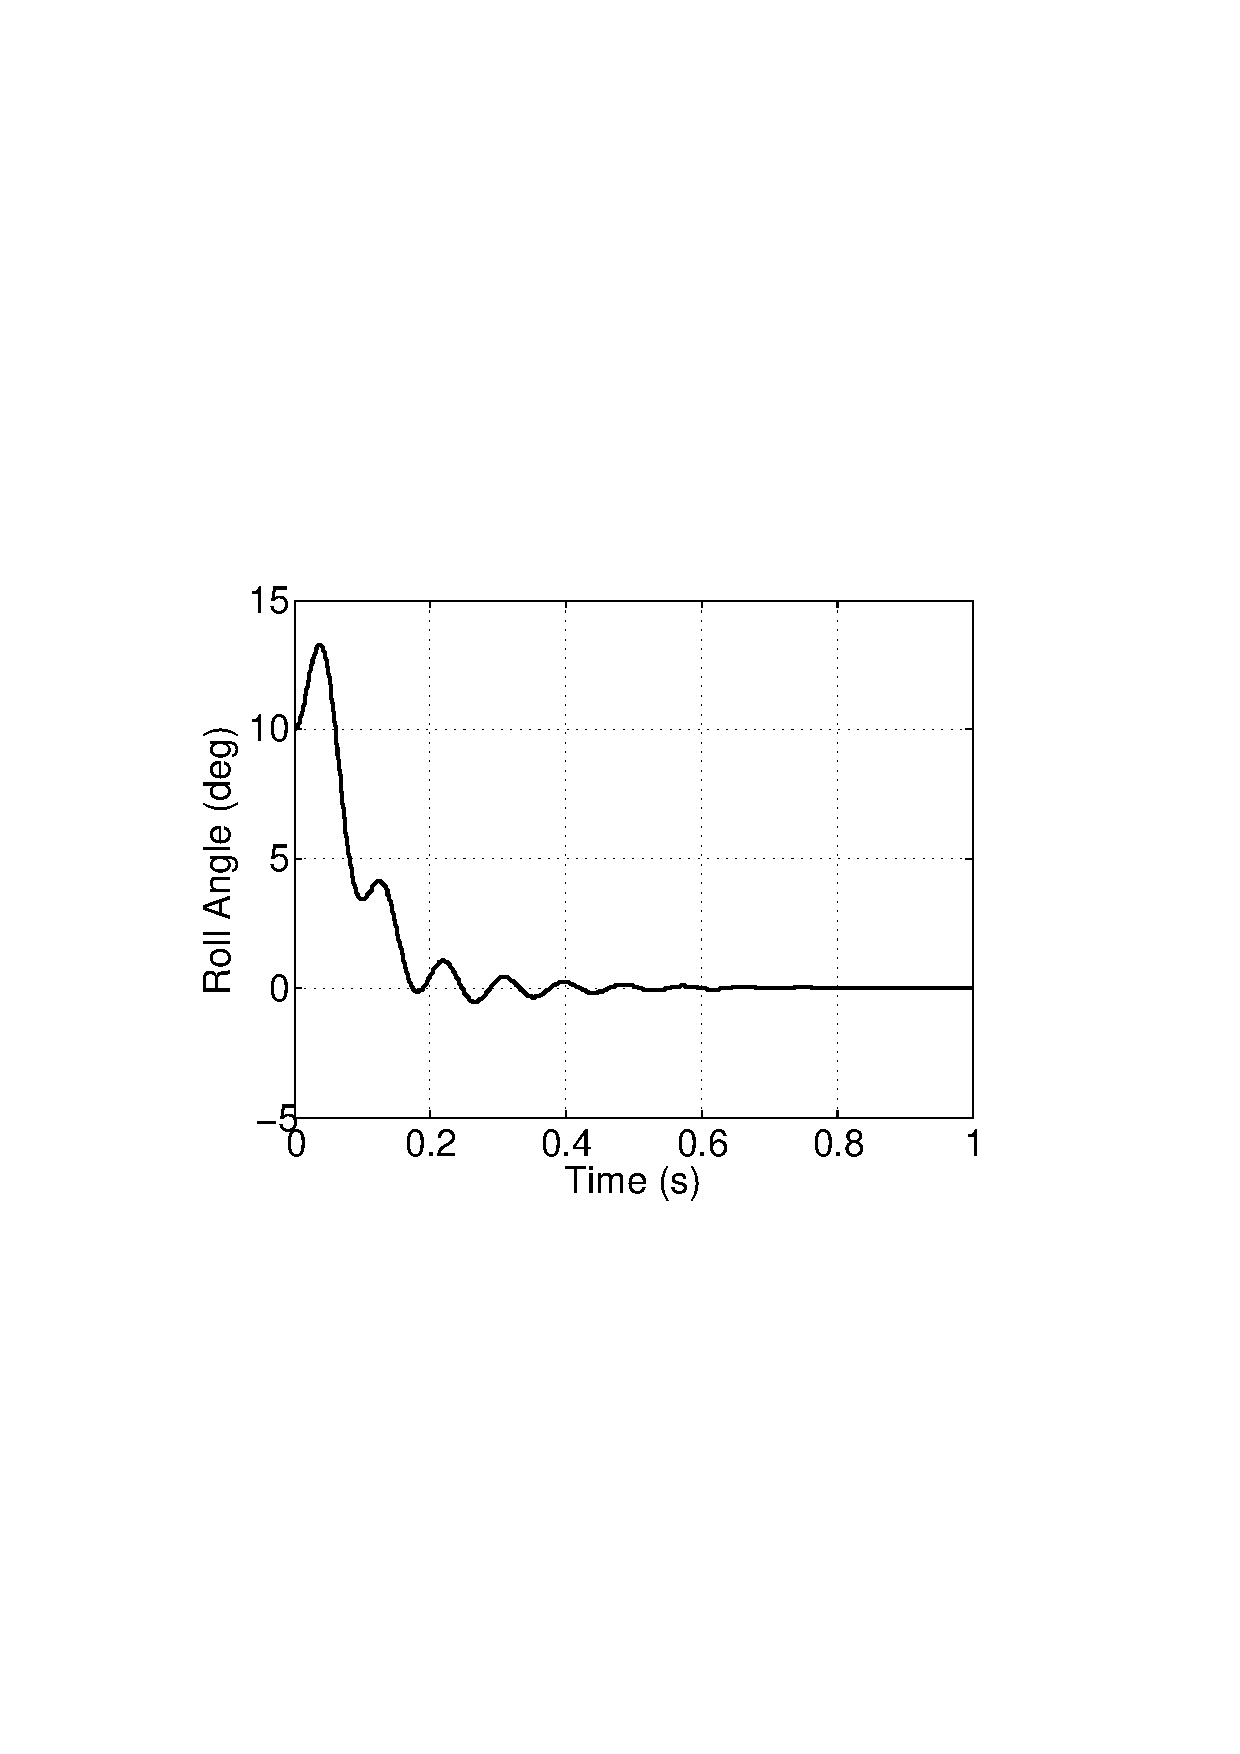
\includegraphics[width=3.7cm]{fig6a}
%\title{Output response}
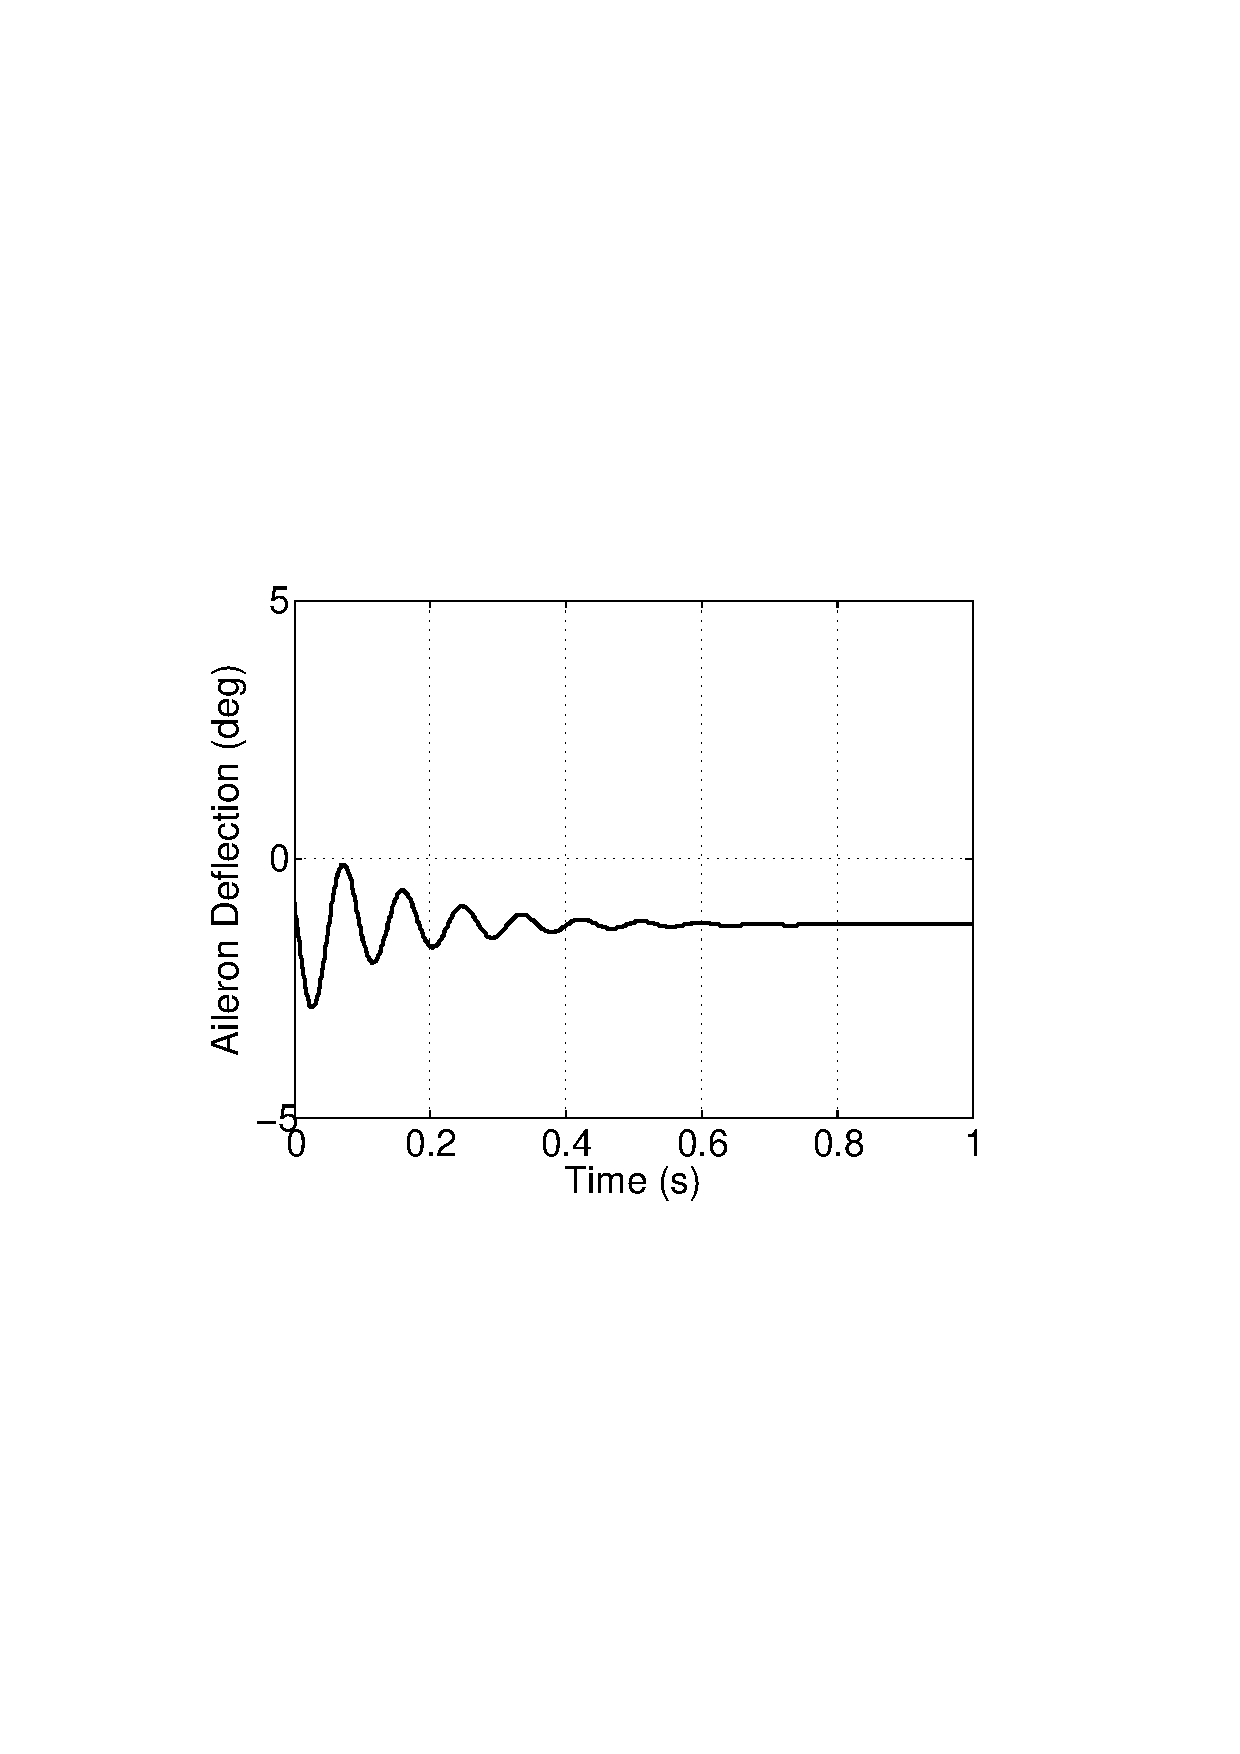
\includegraphics[width=3.7cm]{fig6b}
%\caption{Output response}
%\end{figure}
\begin{center}
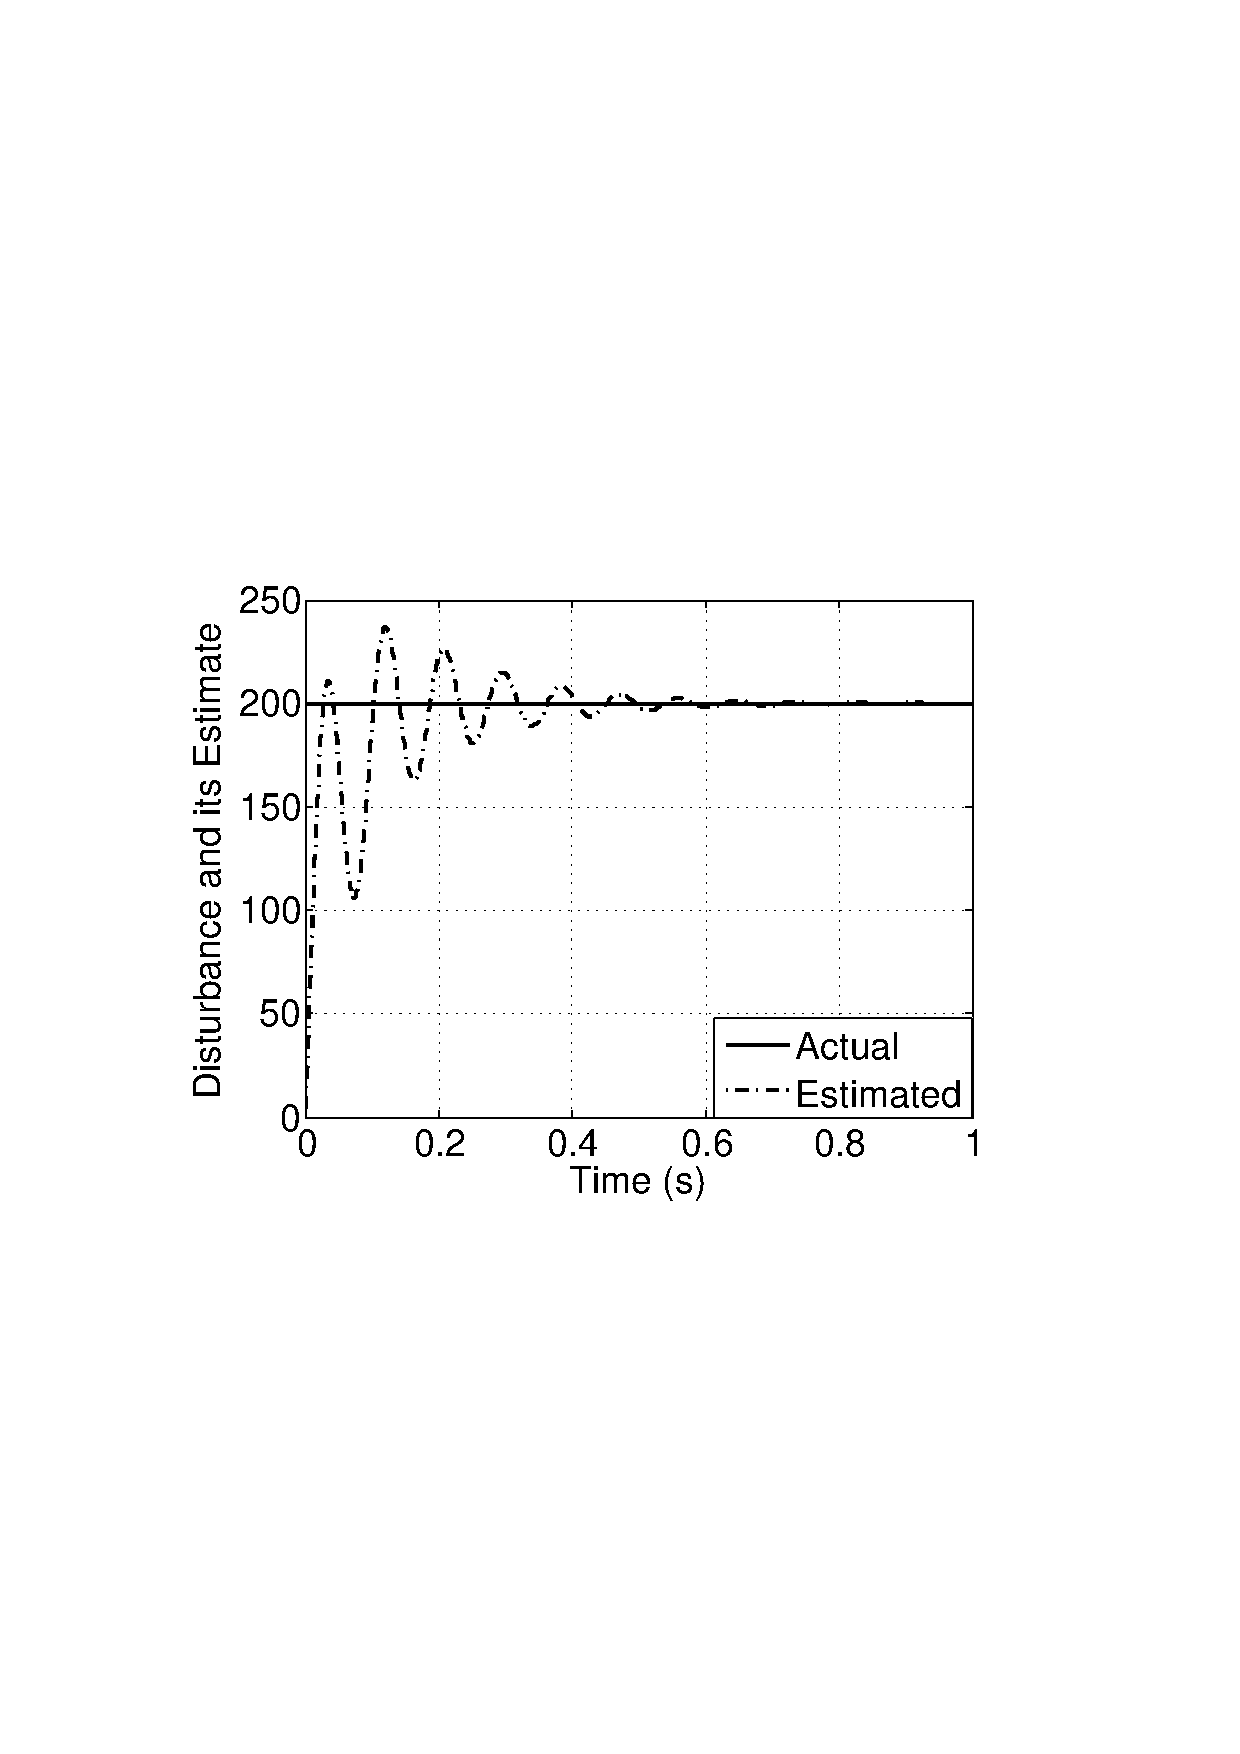
\includegraphics[width=3.4cm]{fig6c}
\end{center}
\end{figure}
\end{frame}
%---------------------------------
\begin{frame}
\frametitle{Performance of UDE based control law with actuator compensation using Method 1}
\textbf{Inference}
\begin{itemize}  % Shows text in bullet point 		
		\item Control effort, though oscillatory was found to be within the desired limits
		\item Disturbance Estimation was found to be satisfactory after 500 ms
		\item The overshoot in output response was dependent on magnitude of disturbance

		%\item The value of $\tau$ was thereby tuned to achieve the best possible performance
\end{itemize}
\end{frame}
%0----------------------------------------------------------------------------------------------------
\subsection{Method 2: Using Compensator Form 1}
\begin{frame}
\frametitle{Method 2: Using Compensator Form 1}
\textbf{The block diagram schematic for this proposed method}
\begin{figure}[h]
\begin{center}
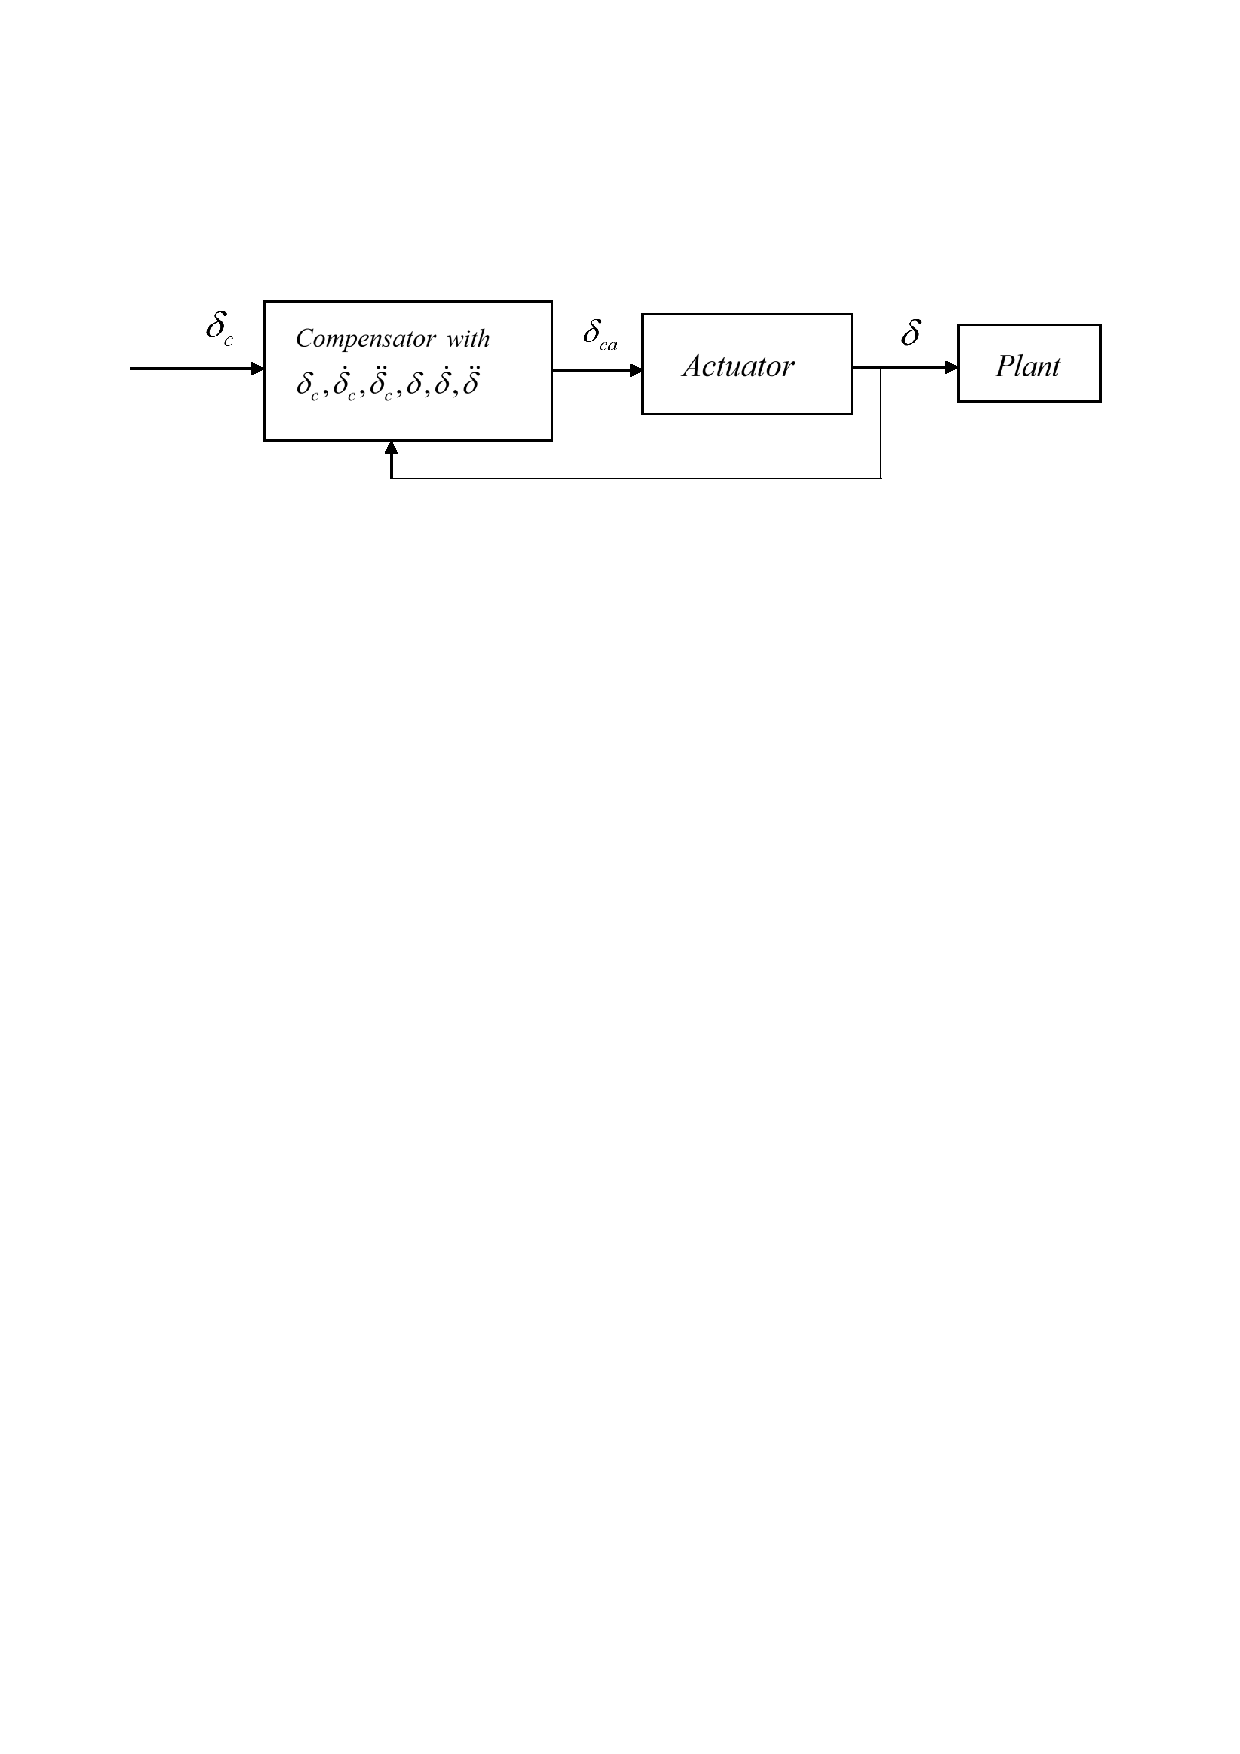
\includegraphics[width=8.4cm]{fig7}    % The printed column width is 8.4 cm.
\end{center}
\end{figure}

\begin{itemize}
\item In this approach, $\delta_c$ is taken as a reference signal which $\delta$ is required to track before it is fed to the plant
\item $\delta_{ca}$ is taken as the compensated control to the actuator
\end{itemize}

\end{frame}
%----------------------------------------------------------------------------------------
\begin{frame}
\frametitle{Method 2: Using Compensator Form 1}
\begin{itemize}
%\item $\de

		\item $\delta_{ca}={{1}\over{\omega^2_A}}(\nu_a+u_{na})$
		\item $u_{na}=2\zeta_A\omega_A\dot{\delta}+\omega_A^2\delta$
		\item $\nu_a=\ddot{\delta_c}  -  k_{a1}\dot{\delta_e} - k_{a2}\delta_e$
		\begin{enumerate}
		\item where $\delta_e=\delta_c-\delta$
		\item $k_{a1}$ and $k_{a2}$ are the feedback gains, whose proper choice will ensure stability

\end{enumerate}
\item This results in tracking error dynamics between $\delta$ and $\delta_c$ of the form $\ddot{\delta_e}  +  k_{a1}\dot{\delta_e} + k_{a2}\delta_e=0$
\end{itemize}
\end{frame}
%------------------------------------------------------------------------------------------------
\begin{frame}
\frametitle{Performance of UDE based control law with actuator compensation using Method 2}
\textbf{Simulation parameters}
\begin{itemize}
\item Using desired settling time to be 50ms, damping ratio to be 0.8, $k_{a1}$ and $k_{a2}$ are evaluated to be 160 and 10000
\item $\tau$ is taken as 0.01 
%\begin{enumerate}
		%\item $\delta_{ca}={{1}\over{\omega^2_A}}(\nu_a+u_{na})$
		%\item $u_{na}=2\zeta_A\omega_A\dot{\delta}+\omega_A^2\delta$
		%\item $\nu_a=\ddot{\delta_c}  -  k_{a1}\dot{\delta_e} - k_{a2}\delta_e$
		%%\item <+-|alert@+>
%\end{enumerate}
\item Other simulation parameters are as per Table 1.
\item Simulations are done with $d_{ext}$ and uncertainty in $\omega_{RR}$
\end{itemize}

\end{frame}
%=====================================================================================================
\begin{frame}
\frametitle{Performance of UDE based control law with actuator compensation using Method 2}
%\textbf{Simulation Results}
\begin{figure}
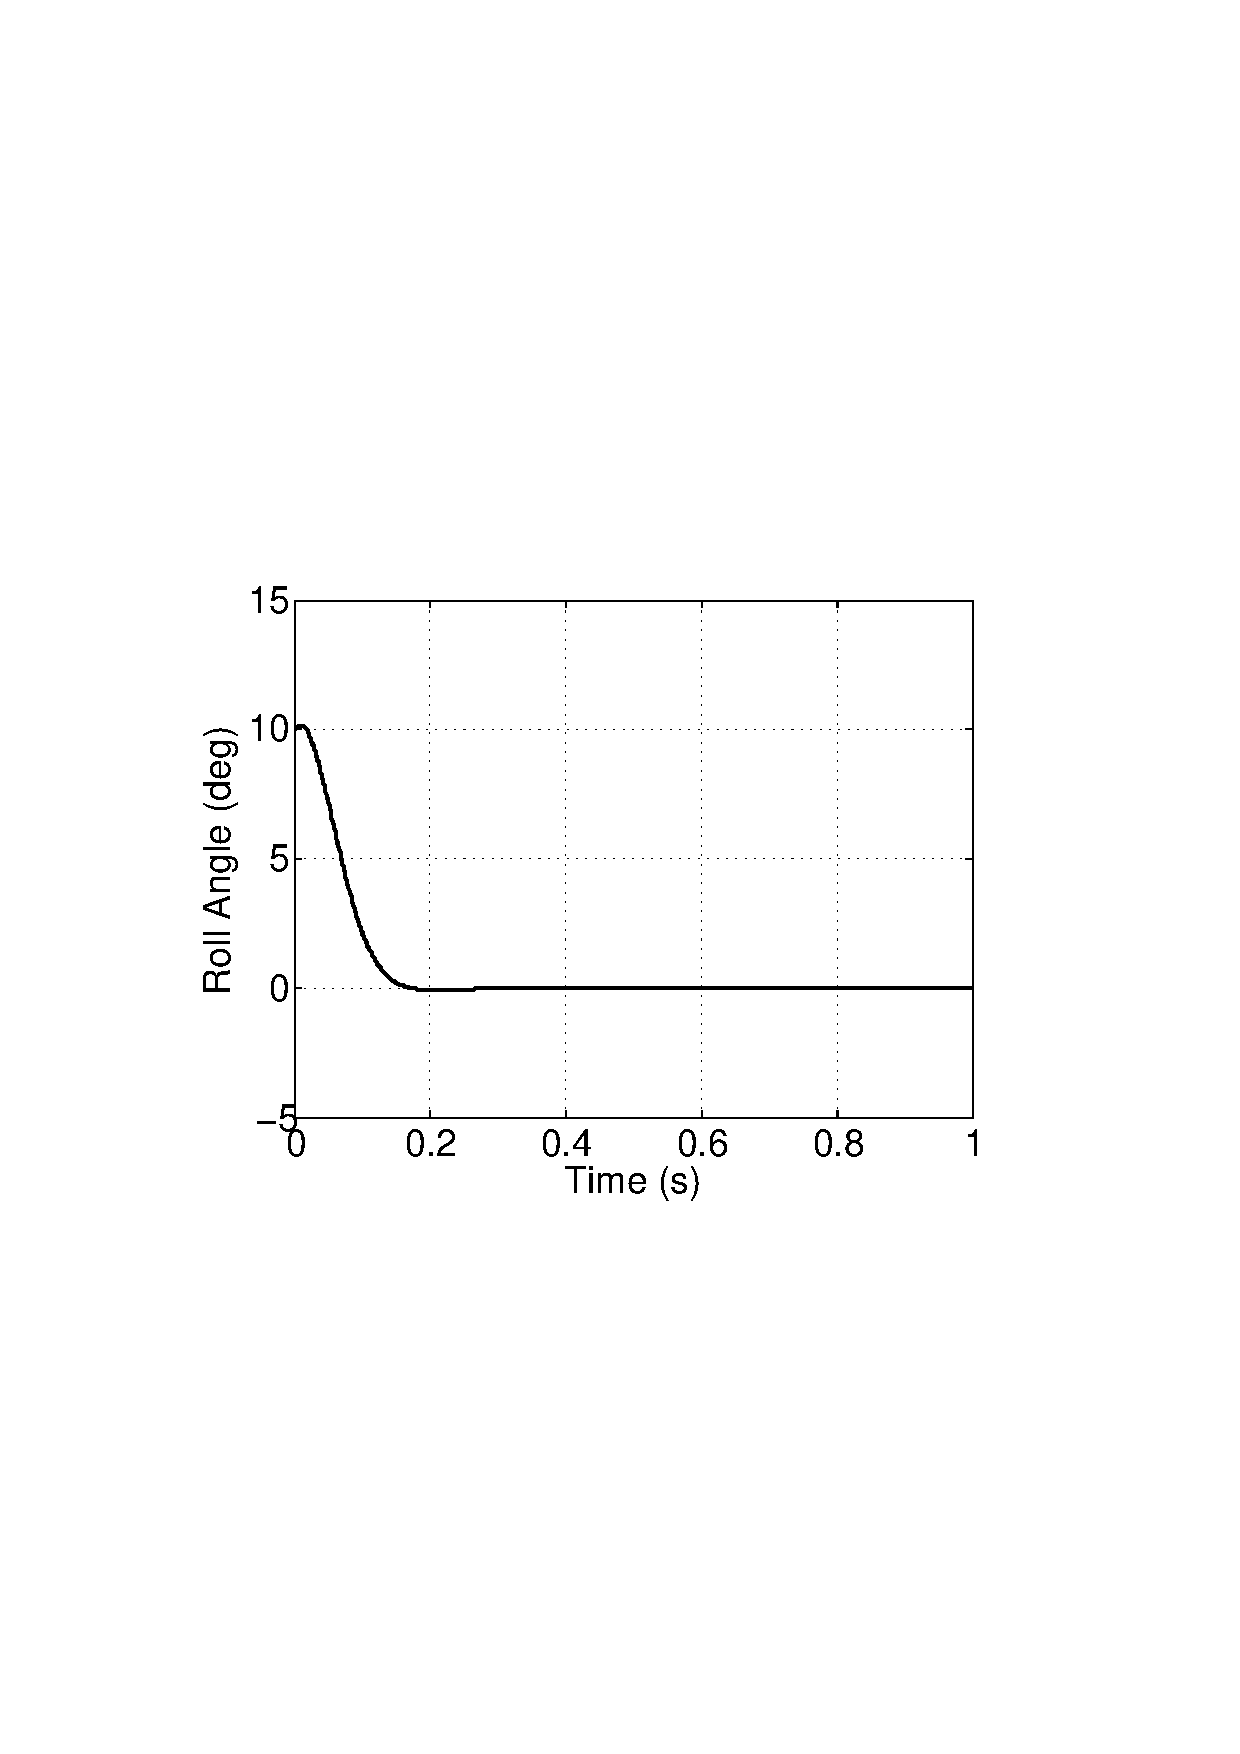
\includegraphics[width=3.7cm]{fig8a}
%\title{Output response}
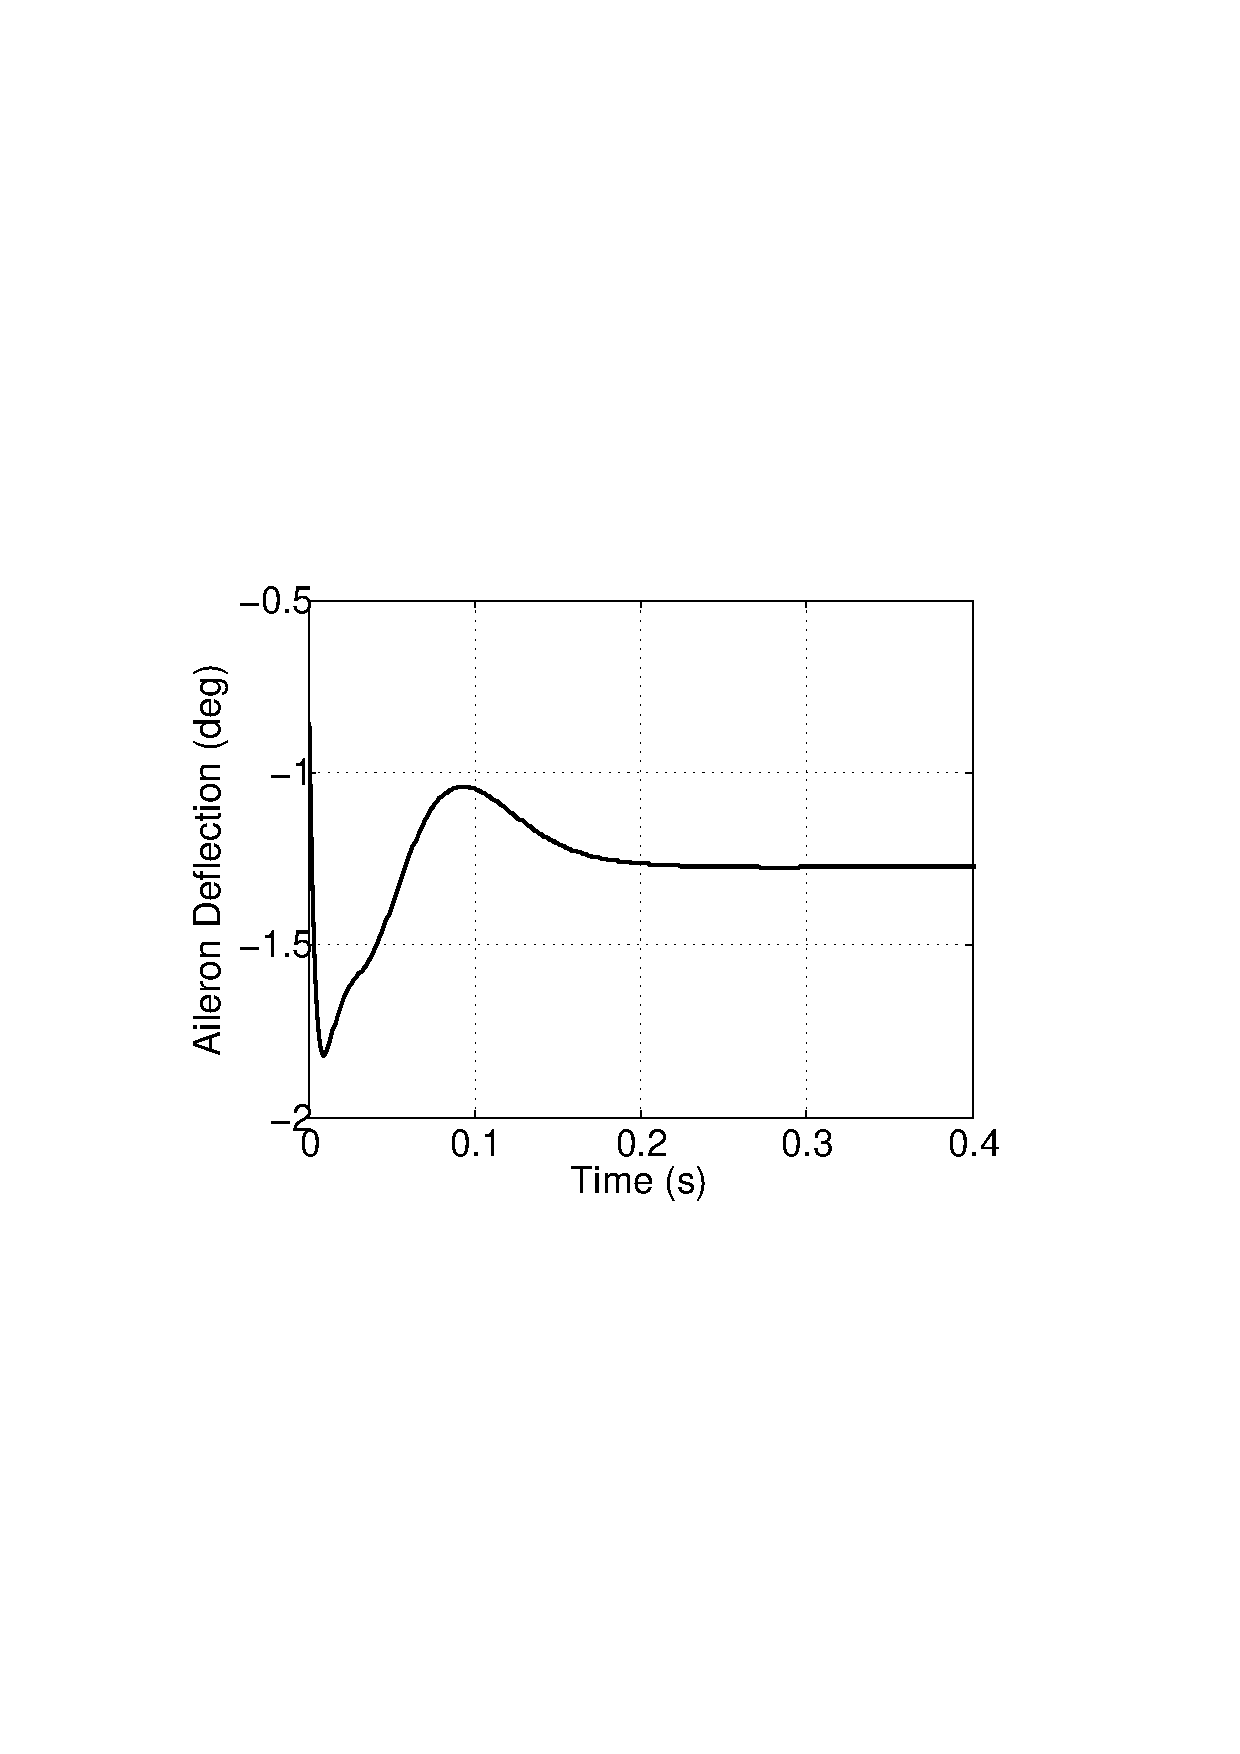
\includegraphics[width=3.7cm]{fig8b}
%\caption{Output response}
%\end{figure}
\begin{center}
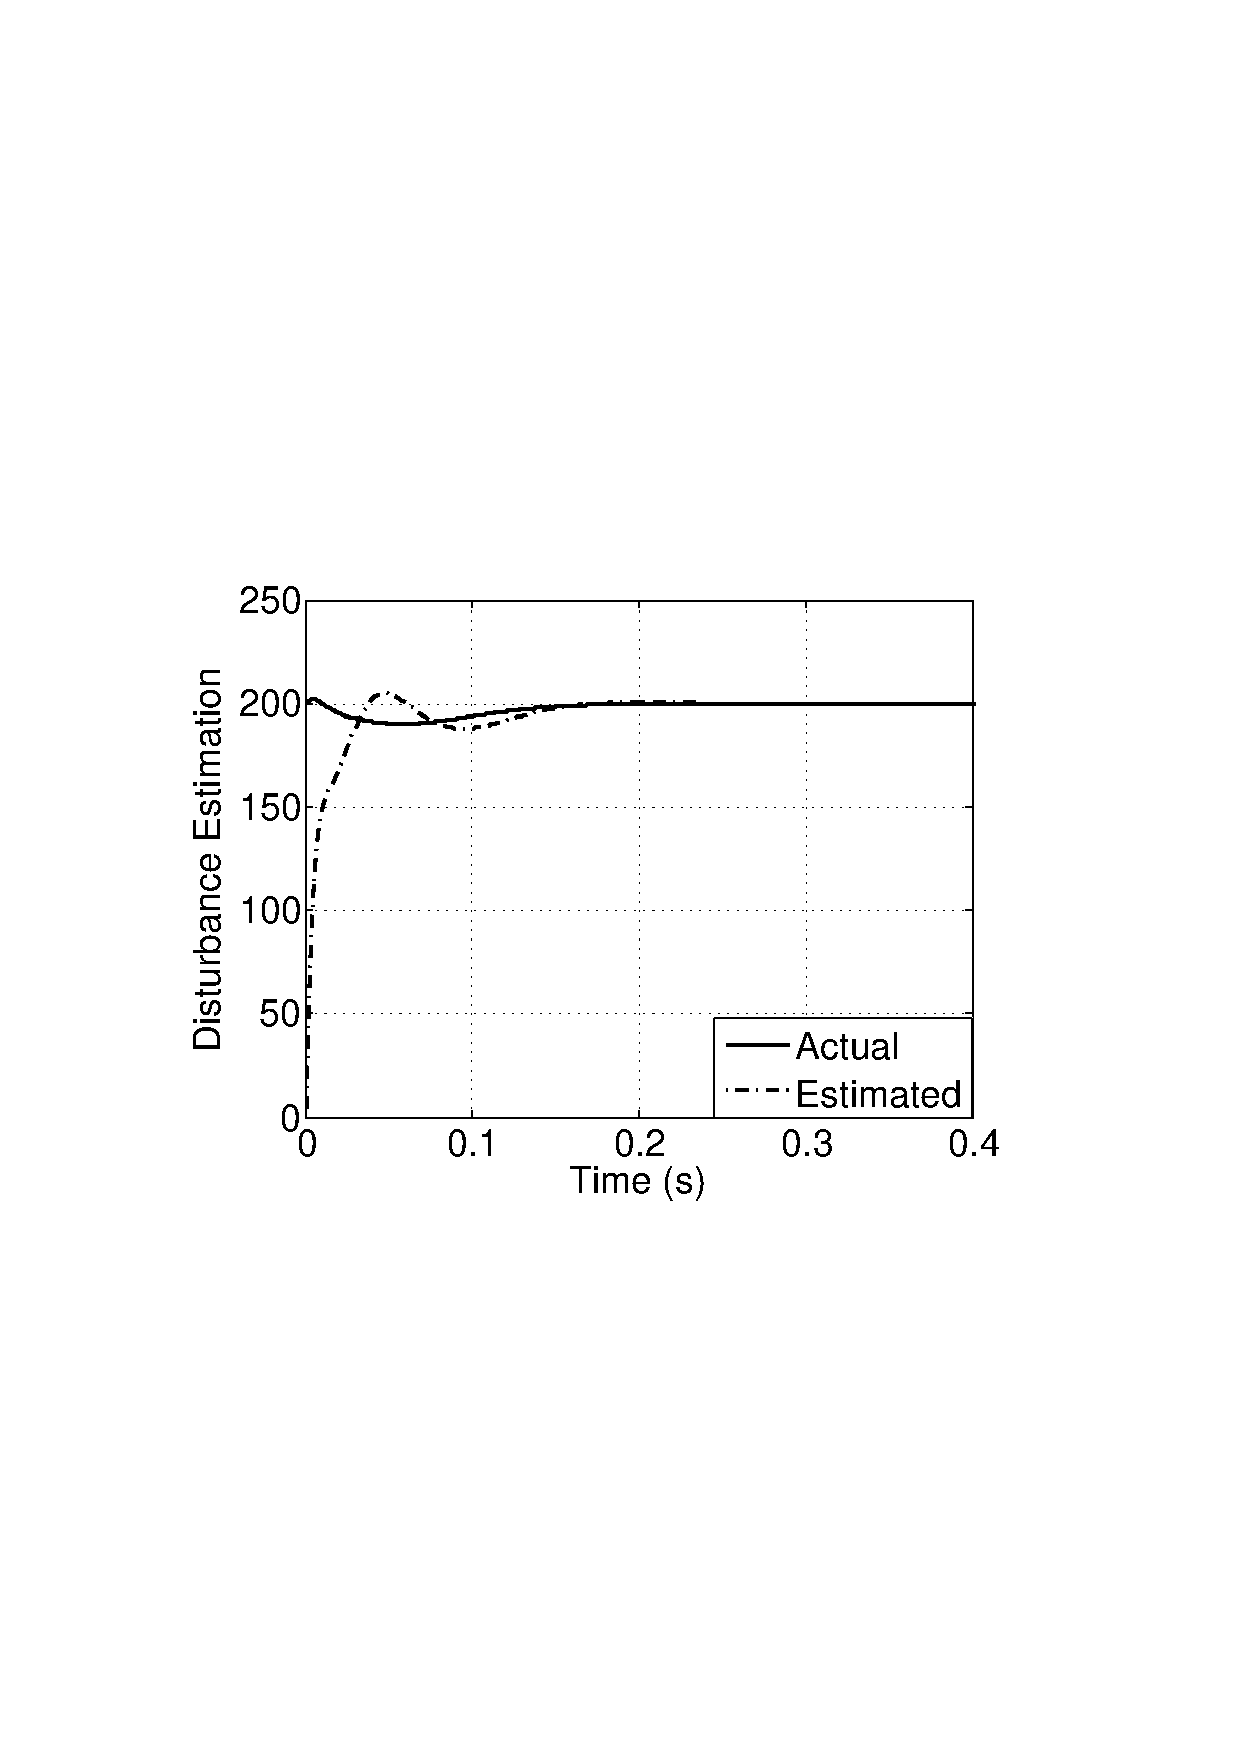
\includegraphics[width=3.4cm]{fig8c}
\end{center}
\end{figure}
\end{frame}
%\end{frame}
%=====================================================================================================
\begin{frame}
\frametitle{Performance of UDE based control law with actuator compensation using Method 2}
\textbf{Inference}
\begin{itemize}
\item The compensator proposed in Method 2 has been successful in ensuring that $\delta$ tracks $\delta_c$
\item However, the drawback of this approach is that it requires first and second derivatives of $\delta$ and $\delta_c$
\item While these derivatives can be assumed to be available for simulation purposes, their availability cannot be assured in real-life situations
\end{itemize}
\end{frame}
%=====================================================================================================
\subsection{Method 3: Using Compensator Form 2}
\begin{frame}
\frametitle{Method 3: Using Compensator Form 2}

\textbf{Block Diagram Schematic for this proposed method}
\begin{figure}[h]
\begin{center}
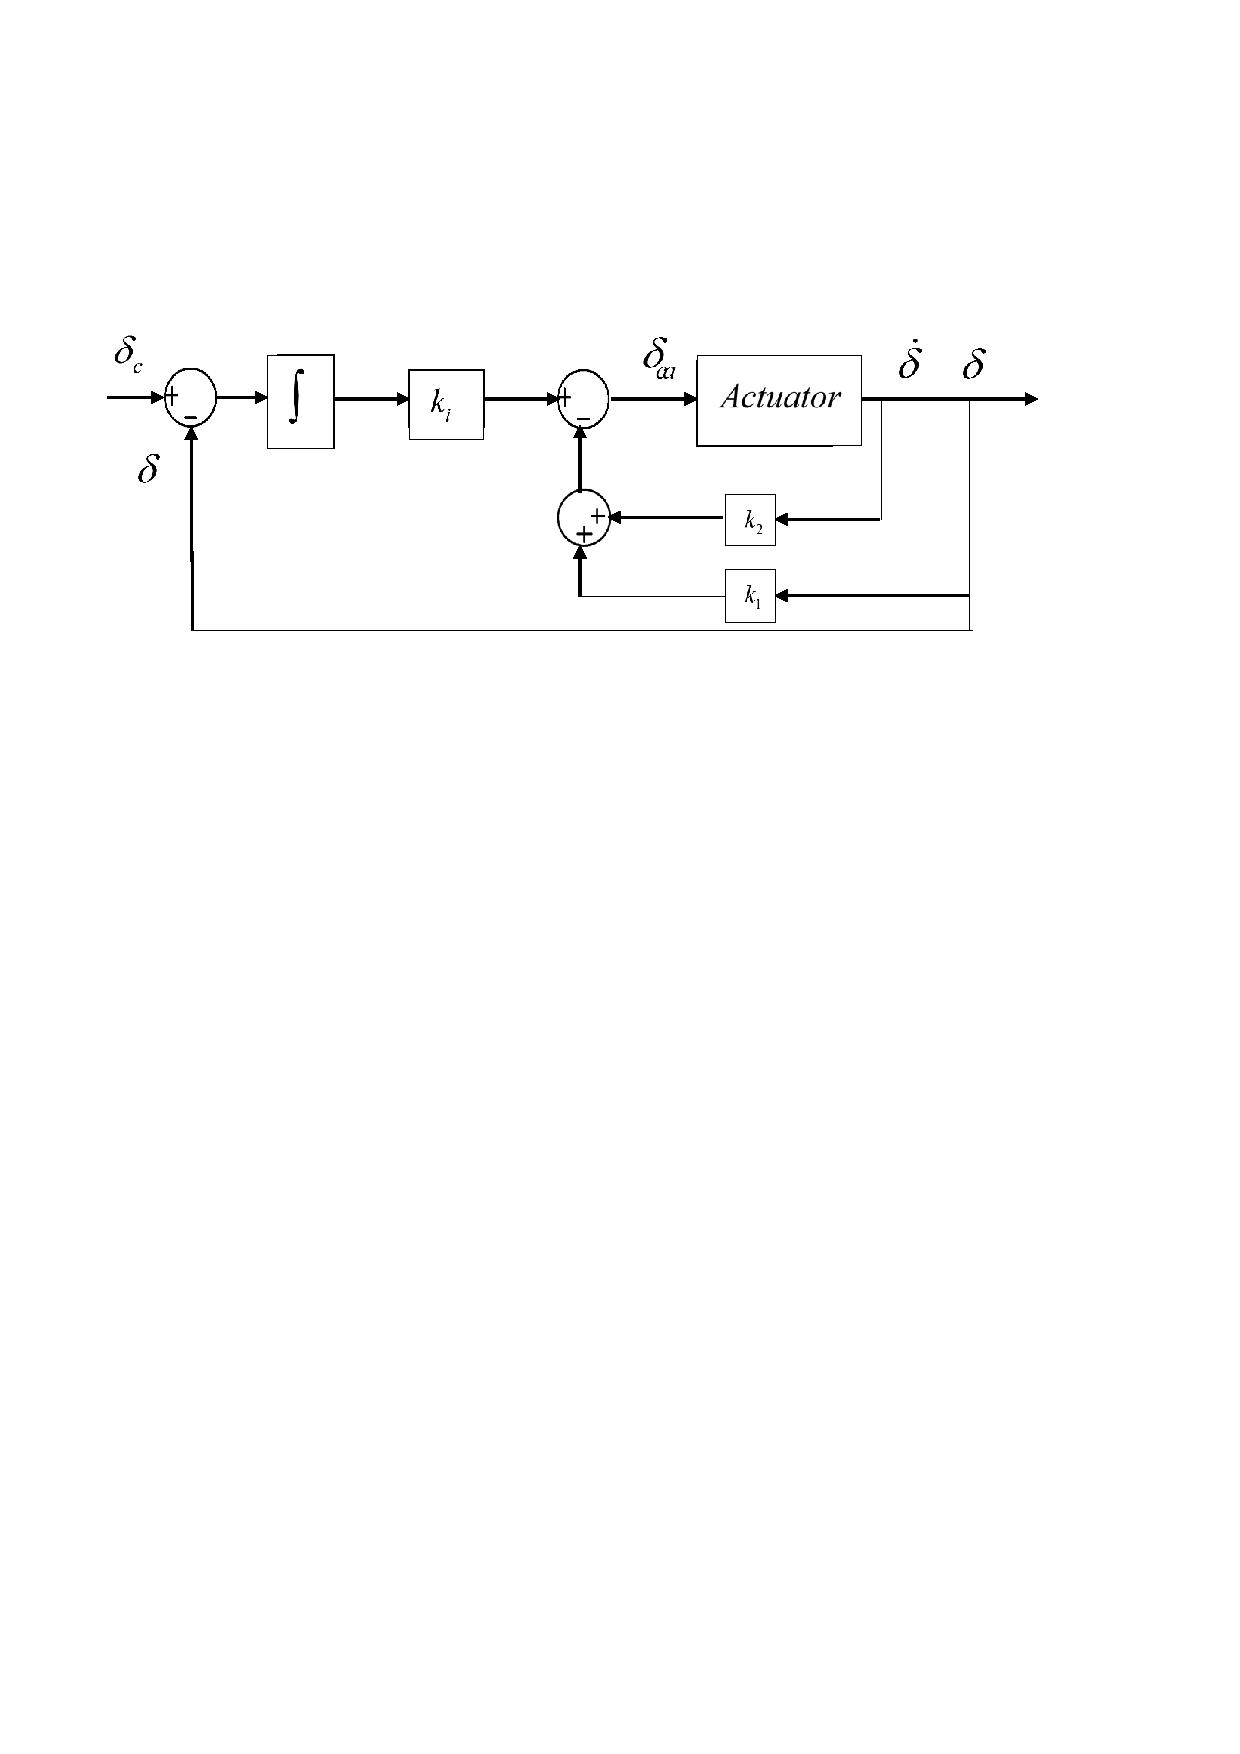
\includegraphics[width=8.4cm]{fig9}   % The printed column width is 8.4 cm.
\end{center}
\end{figure}
The proposed compensator in this strategy not only reduces the number of derivatives of $\delta$ and $\delta_c$ required, it also ensures that $\delta$ tracks $\delta_c$.

In this proposed strategy, $\delta_{ca}$ is the compensated actuator input.
\end{frame}
%=====================================================================================================
\begin{frame}[shrink]
\frametitle{Method 3: Using Compensator Form 2}
\textbf{Deducing expression for $\delta_{ca}$}
As referred from \cite{ogata2010}, 
%the expression for compensated actuator input $\delta_{ca}$ can be expressed as ;
%%
%\begin{equation*}
%\delta_{ca}=-k_1\delta-k_2\dot{\delta}+k_i\int[\delta_c-\delta]dt
%%\label{eq21}
%\end{equation*}
%%
The transfer function of the second order actuator can be written as;
%
\begin{equation*}
%\delta_{ca}={{1}\over{\omega^2_A}}(\nu_a+u_{na})
{{\delta (s)}\over{\delta_c(s)}} = {{b}\over{s^2 + as + b}}
%\label{eq22}
\end{equation*}
%
with $b=\omega_A^2$ and $a=2\zeta_A\omega_A$. The actuator dynamics can be re-written in the state space model as follows;
%
\begin{eqnarray*}
\dot{x} &=& Ax+Bu \nonumber \\
y &=& Cx
%\label{eq23}
\end{eqnarray*}
A, B and C are the matrices of the system and are given by
$$
A=\left[
\begin{array}{cccc}
0 & 1\\
-b & -a\\
\end{array}\right]; 
%$$
%$$
B=\left[
\begin{array}{cccc}
0 \\
b\\
\end{array}\right]; 
%$$
%$$
C=\left[
\begin{array}{cccc}
1 & 0\\
0 & 1\\
\end{array}\right]
$$
%
\end{frame}
%=====================================================================================================
\begin{frame}
\frametitle{Method 3: Using Compensator Form 2}
The compensated actuator control input $\delta_{ca}$ is thus defined as follows;
%
\begin{equation*}
u= \delta_{ca}= -k_1\delta -k_2\dot{\delta} +k_i \int{(\delta_c-\delta)}dt
%\label{eq24}
\end{equation*}
\end{frame}
%=====================================================================================================
\begin{frame}
\frametitle{Method 3: Using Compensator Form 2}
\textbf{Determination of feedback gains $k_1$, $k_2$ and $k_i$}

\begin{itemize}
\item The desired characteristic equation for this system is of the form $(s^2+ 2\zeta_d\omega_ds+ \omega_d^2)(s+ \zeta_d\omega_d)=0$
\begin{enumerate}
\item damping factor 0.8
\item to ensure that the compensator is faster than the actuator, its desired settling time should be less than actuator settling time
\end{enumerate}
\item To derive the actual characteristic equation for this system, following \cite{ogata2010}, we first need to define matrices $\hat A$, $\hat B$, $\hat K$;
%\begin{enumerate}
%\item 
%\end{enumerate}
\item Computing $sI-(\hat A-\hat B\hat K)=0$ results in the actual characteristic equation of the form $s^3+s^2(a+bk_2)+s(b+bk_1)+bk_i=0$
\item Comparing the desired and actual characteristic equations, gives us the value of $k_1$, $k_2$ and $k_i$
\end{itemize}
\end{frame}
%=====================================================================================================
\begin{frame}
\frametitle{Performance of UDE based control law with actuator compensation using Method 2}
Simulations were carried with data from Table 1. with an external disturbance $d_{ext}$ present.

\textbf{Desired compensator settling time : 12.5ms}
\begin{itemize}
\item First a desired settling time of 1/4th that of actuator settling time, i.e. 12.5ms is chosen. 
		%\begin{enumerate}
		\item for this value, with damping ratio of 0.8, $k_1$, $k_2$ and $k_i$ were calculated to be 35.48, 0.083, 5120, respectively
		%\end{enumerate} 
\end{itemize}
%\item Simulation results 
\end{frame}
%----------------------------------------------------------------
\begin{frame}
\frametitle{Performance of UDE based control law with actuator compensation using Method 2}
\textbf{Simulation results for desired compensator settling time : 12.5ms}
\begin{figure}[h]
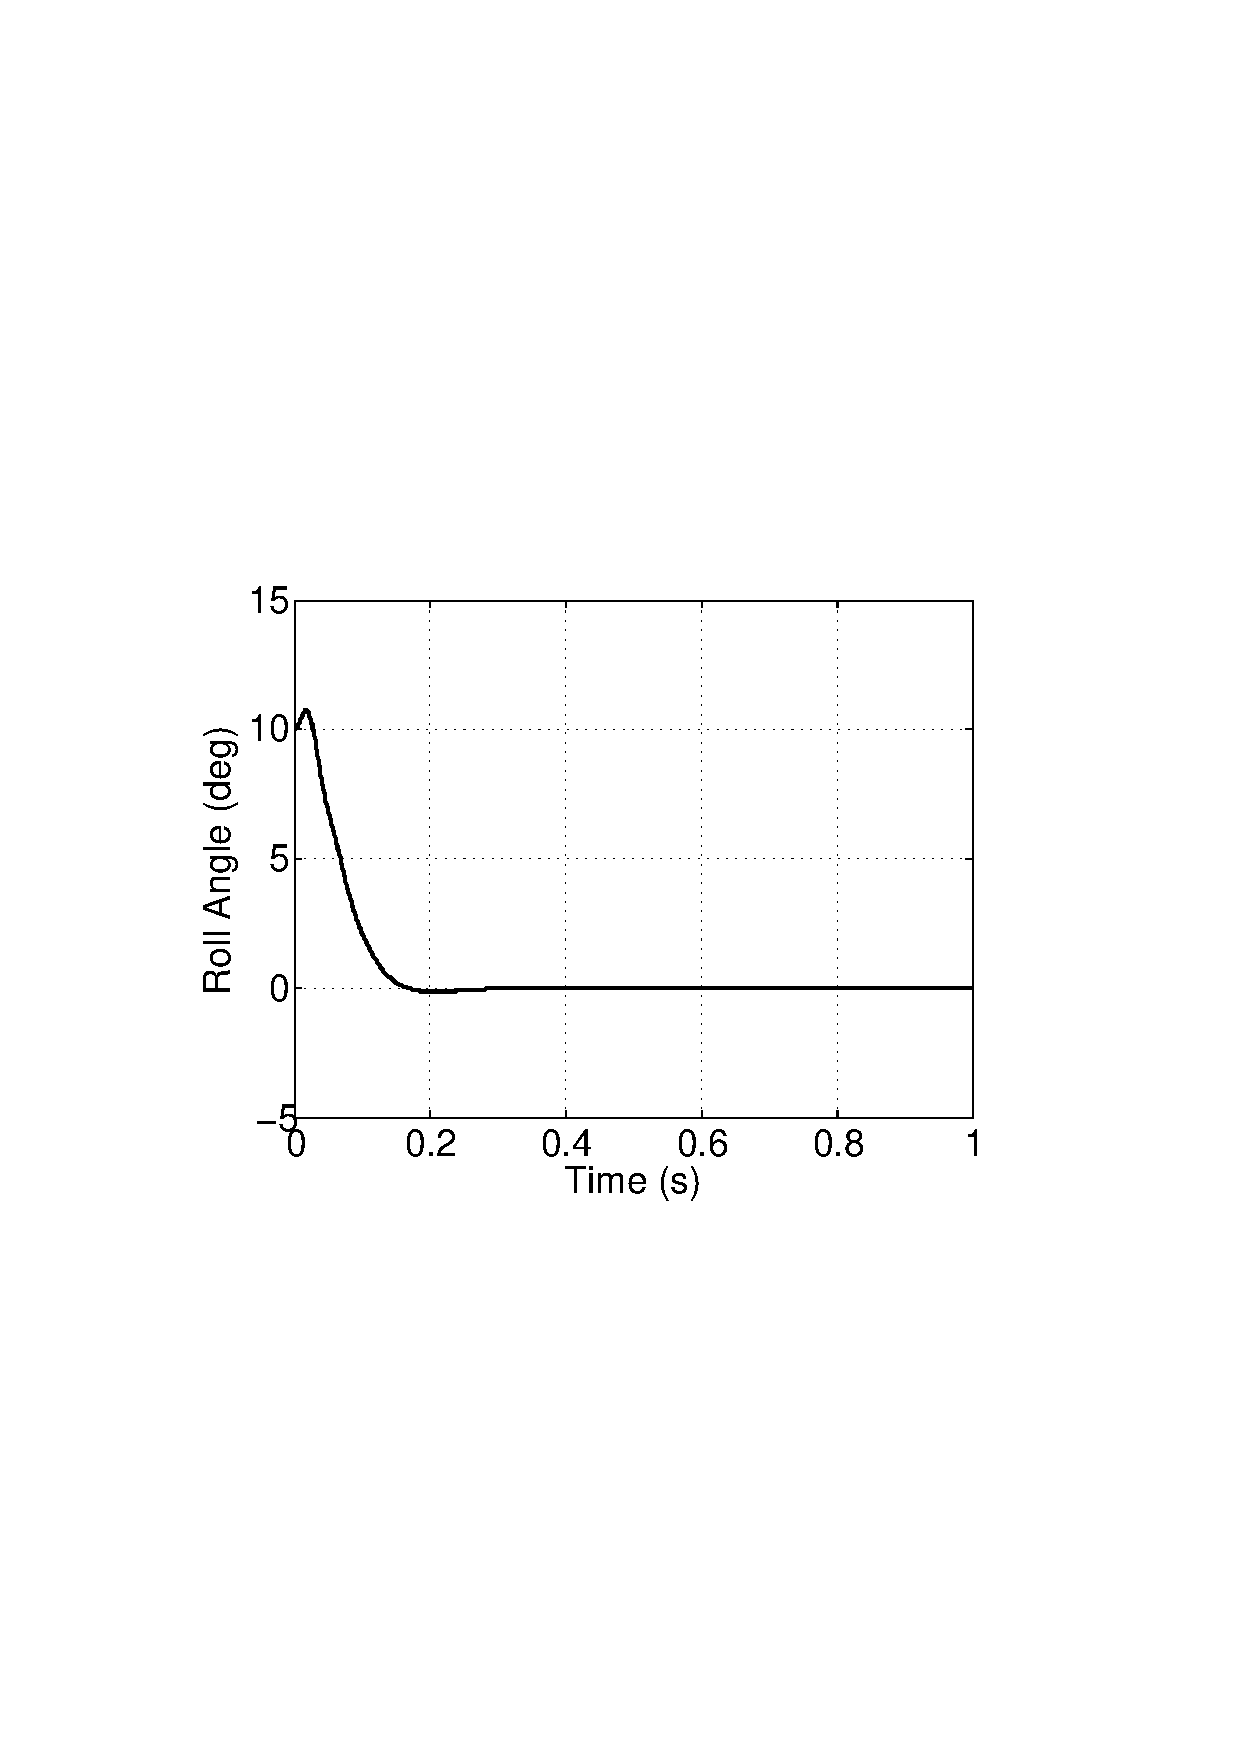
\includegraphics[width=3.3cm]{fig10a}
%\title{Output response}
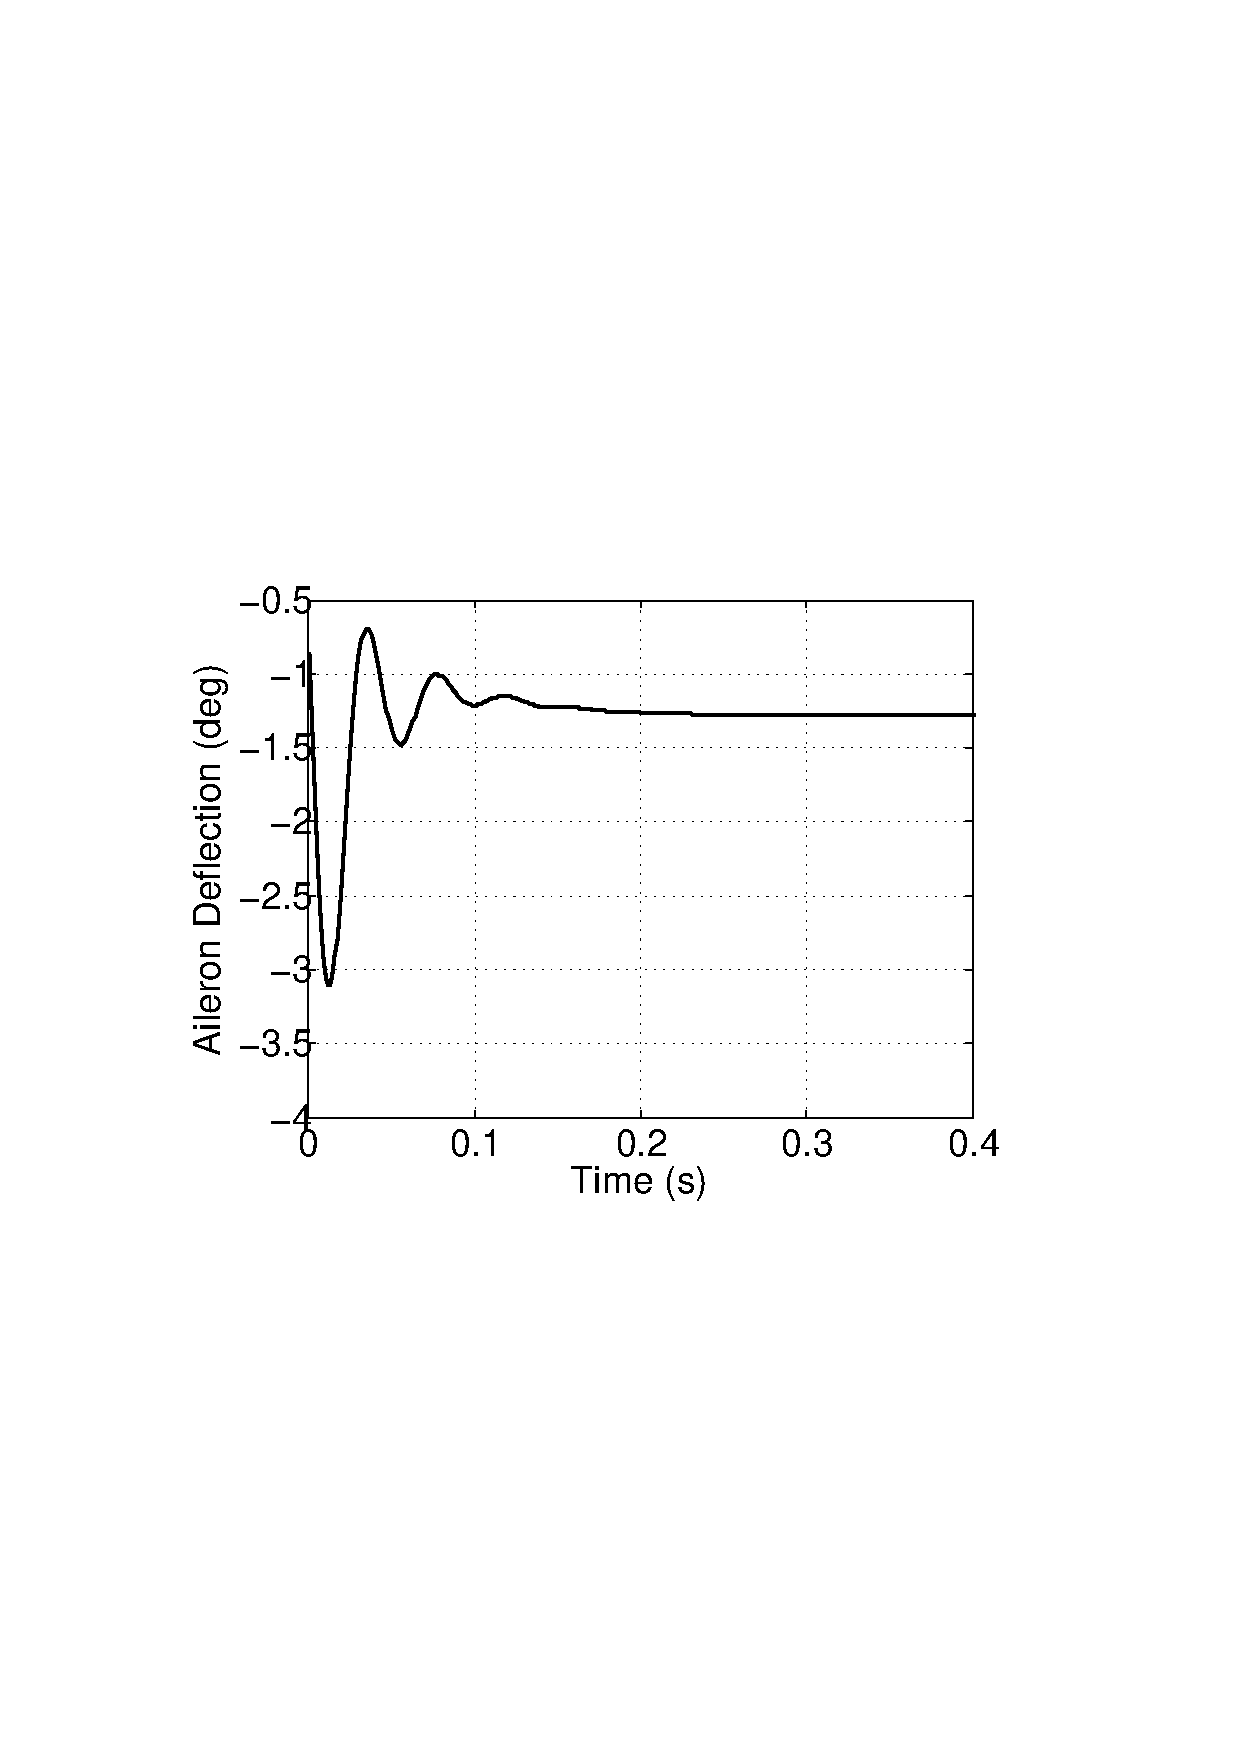
\includegraphics[width=3.3cm]{fig10b}
%\caption{Output response}
\end{figure}
%\begin{center}
\begin{figure}
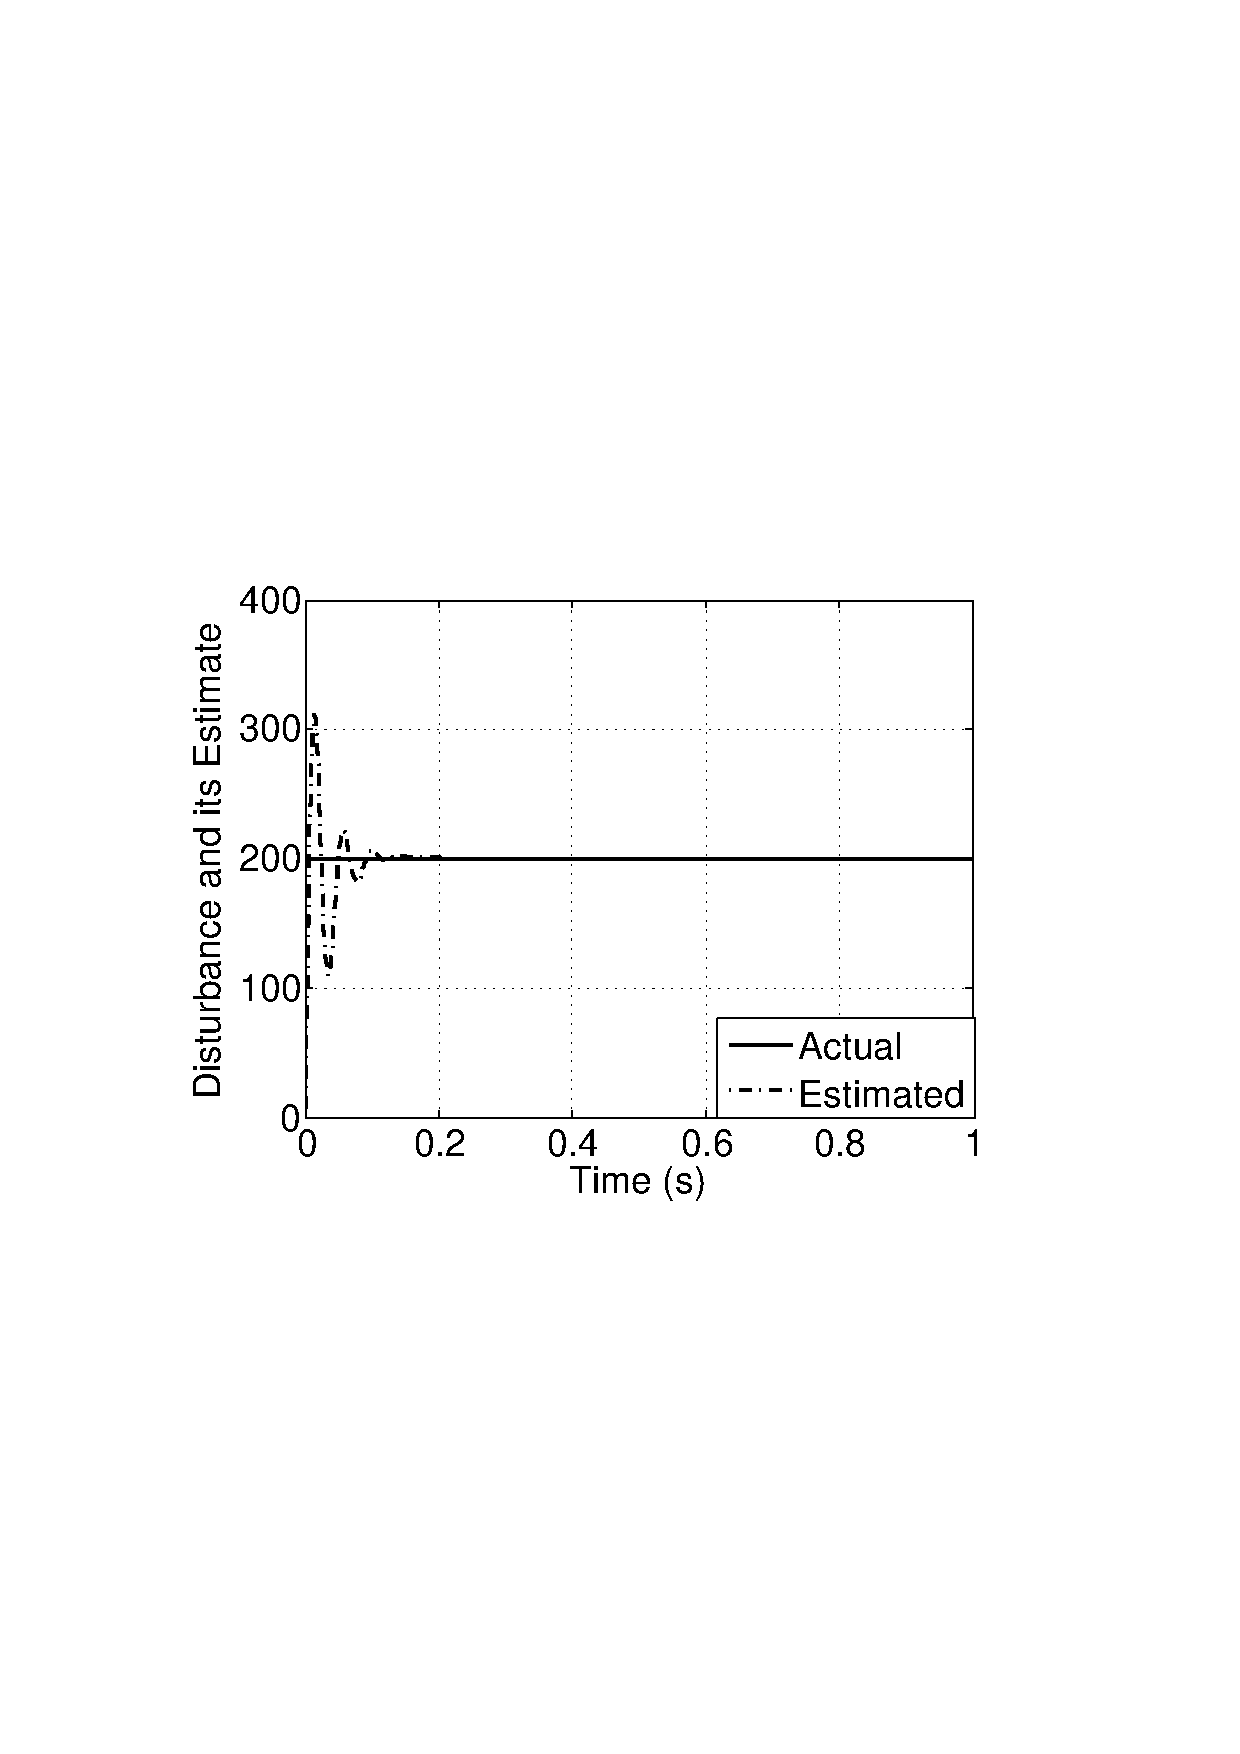
\includegraphics[width=3.3cm]{fig10c}
%\end{center}
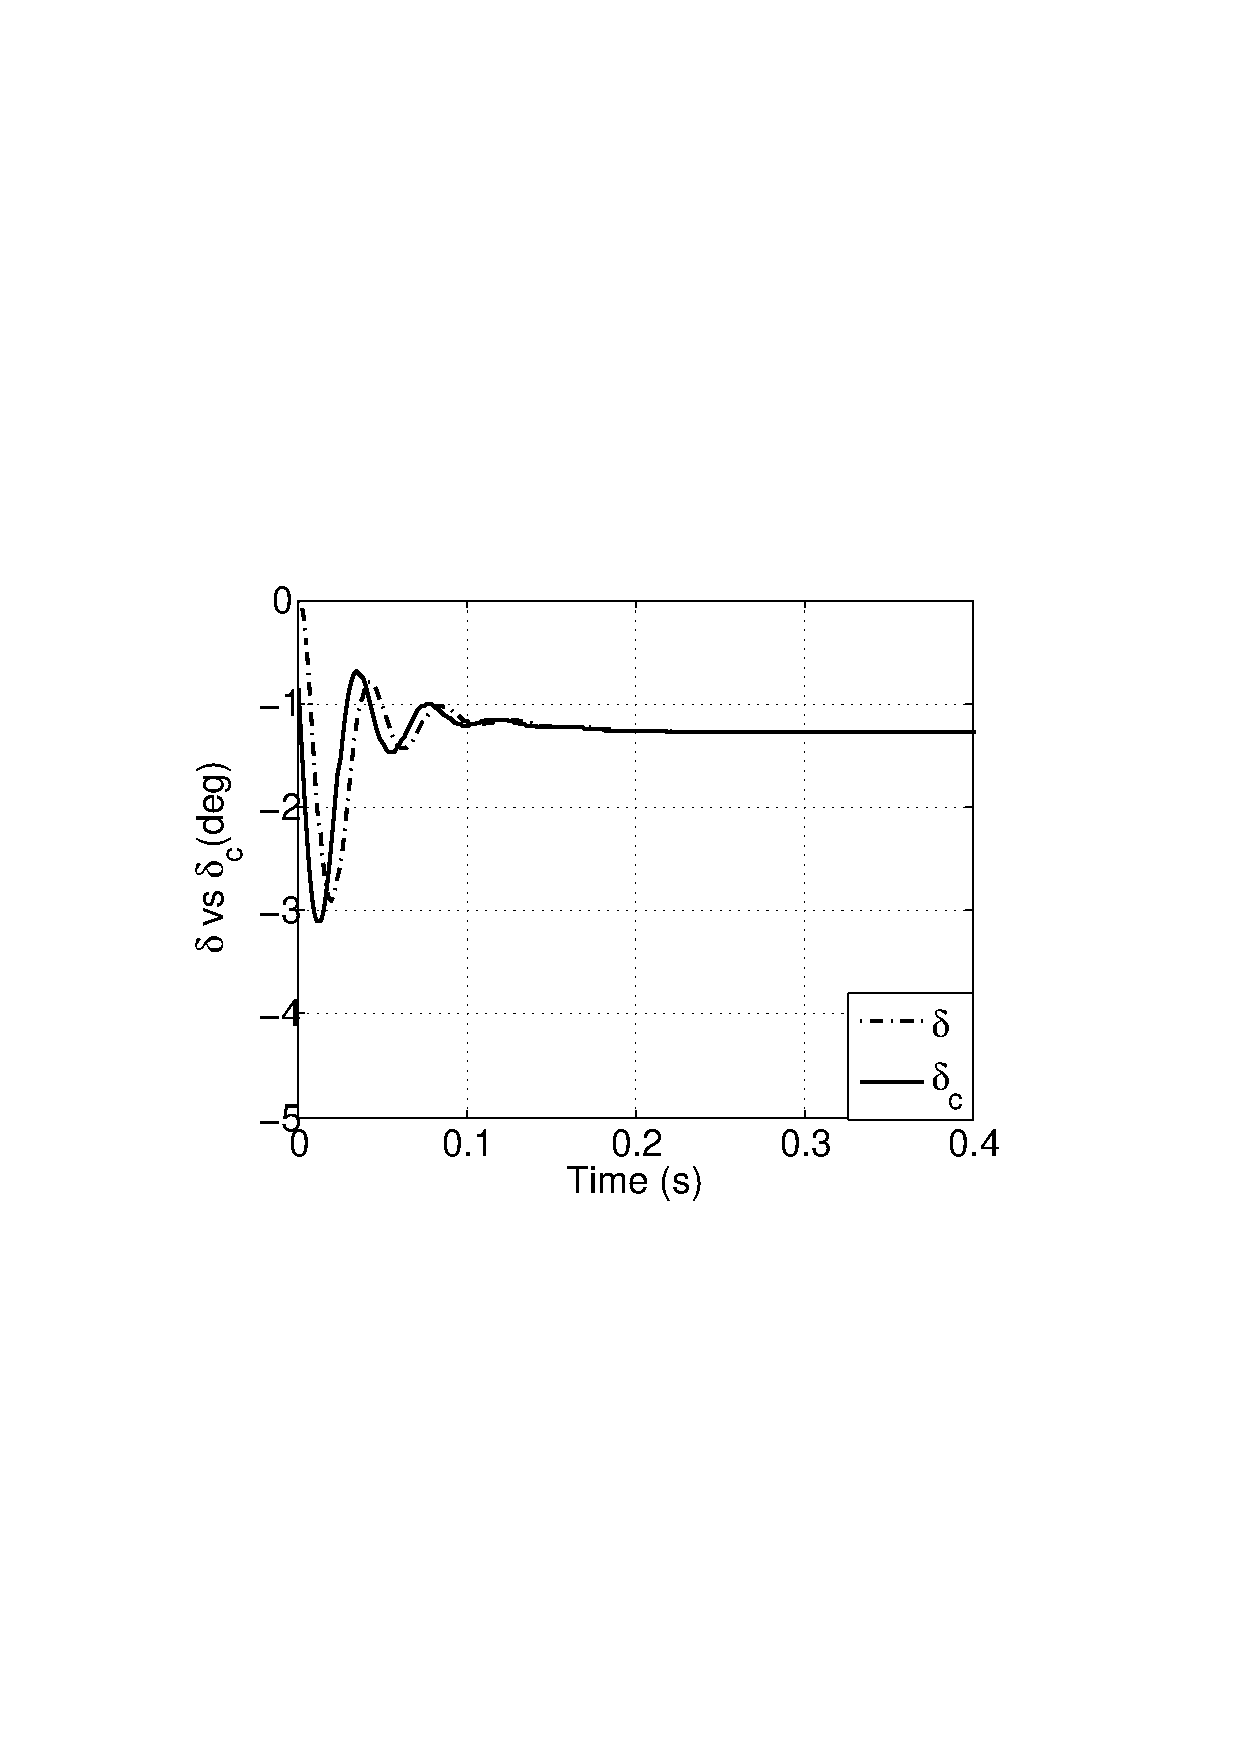
\includegraphics[width=3.3cm]{fig10d}
\end{figure}
\end{frame}
%=====================================================================================================
\begin{frame}
\frametitle{Performance of UDE based control law with actuator compensation using Method 2}
Simulations were carried with data from Table 1. with an external disturbance $d_{ext}$ present.

\textbf{Desired compensator settling time : 7.96ms}
\begin{itemize}
\item It was observed that for a given damping ratio, say 0.8, the relation between $\tau$ and settling time for the error dynamics ($t_s$) can be expressed as $\tau=1.25 t_s$.
\item For $\tau=0.01$, the desired settling time was computed to be 7.96 ms.
		%\begin{enumerate}
		\item for this value, with damping ratio of 0.8, $k_1$, $k_2$ and $k_i$ were calculated to be 88.89, 0.137 and 19800, respectively
		\item an uncertainty of -30 \% in $\omega_{RR}$ and +30 \% in $K_{\delta}$ along with $d_{ext}$ were introduced
		%\end{enumerate} 
\end{itemize}
%\item Simulation results 
\end{frame}
%----------------------------------------------------------------
\begin{frame}
\frametitle{Performance of UDE based control law with actuator compensation using Method 2}
\textbf{Simulation results for desired settling time : 7.96ms}
\begin{figure}[h]
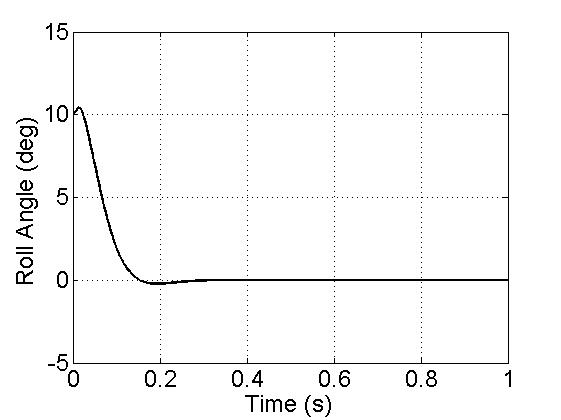
\includegraphics[width=3.3cm]{fig11a}
%\title{Output response}
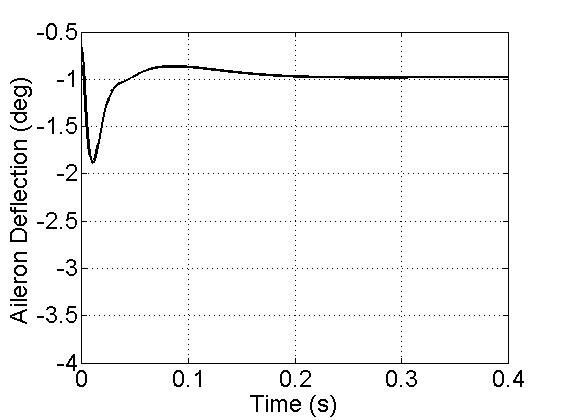
\includegraphics[width=3.3cm]{fig11b}
%\caption{Output response}
\end{figure}
%\begin{center}
\begin{figure}
\includegraphics[width=3.3cm]{fig11c}
%\end{center}
\includegraphics[width=3.3cm]{fig11d}
\end{figure}
\end{frame}
%--------------------------------------------------------------
\begin{frame}
\frametitle{Performance of UDE based control law with actuator compensation using Method 3}
\textbf{Inference}
\begin{itemize}
\item The compensator proposed in Method 3 has been successful in ensuring that $\delta$ tracks $\delta_c$
\item As compared to the previous approach, the number of derivatives of $\delta$ and $\delta_c$ required has been reduced
\item We now require only the control input $\delta_c$, actuator output $\delta$ and its first derivative $\dot{\delta}$
\end{itemize}
\end{frame}
%-------------------------------------------------------------------------------------------------
\section{Conclusion and future work}
\begin{frame}
\frametitle{Conclusion and future work}
\textbf{Our work has proposed three strategies for compensating actuator lag;}
\begin{itemize}  % Shows text in bullet point 		
		%\item The proposed methodology of actuator compensation by tuning the value of filter constant $\tau$, though promising, needs further study
		\item The strategy of tuning filter constant $\tau$, though promising, requires a formula linking $\tau$ with the parameters of the plant or the performance indices
		\item Compensator Form 1, though satisfactory in ensuring tracking of $\delta_c$ by $\delta$, required a number of their derivatives
		\item Compensator Form 2, which gave the desired results at the same time reducing the number of derivatives required	%\item The value of $\tau$ was thereby tuned to achieve the best possible performance
\end{itemize}
\textbf{Our future work would include the following}
\begin{itemize}  % Shows text in bullet point 		
		%\item The proposed methodology of actuator compensation by tuning the value of filter constant $\tau$, though promising, needs further study
		\item Further investigation into the role of filter time constant $\tau$ in actuator compensation
		\item Design of UDE based control law to cater to time varying uncertainties and disturbances along with actuator compensation
		\item Applicability of the proposed methods for non-linear roll dynamics
		%\item The value of $\tau$ was thereby tuned to achieve the best possible performance
\end{itemize}


\end{frame}
%a.org]{\color{blue} helpdesk@e-yantra.org \color{black}} 
%\end{frame}
%%----------------------------------------------------------------------------------------

	\begin{thebibliography}{1}



%\bibitem{IEEEhowto:kopka}
%H.~Kopka and P.~W. Daly, \emph{A Guide to \LaTeX}, 3rd~ed.\hskip 1em plus
  %0.5em minus 0.4em\relax Harlow, England: Addison-Wesley, 1999.
	%
%% Reference 1
%\bibitem{song2002}
%Chanho Sung, and Yoon-Sik Kim, \lq \lq A new approach to motion modeling and autopilot design of skid-to-turn missile," Trans. on Control, Automation, and System Engg, 4(3), Sep 2002, pp. 231-238. 
%
%% Reference 2
%\bibitem{kang2009}
%S. Kang, and H. J. Kim, \lq \lq Roll-pitch-yaw integrated robust autopilot design for a high angle-of-attack missile," J. of Guidance, Control, and Dynamics, Sep-Oct 2009, pp. 1622-1628.
%
%%Reference 3
%\bibitem{sirisha2012}
%C. V. Sirisha, Ranajit Das, and R. N. Bhattacharjee, \lq \lq Disturbance estimation based roll autopilot design for tactical missiles," Proc. Advances in Control and Optimization of Dynamic Systems, ACDOS - 2012, pp. 1-5.

%%Reference 4
%\bibitem{luo2015}
%D. Luo, and Y. Liu, \lq \lq Roll autopilot using variable structure control based on new reaching law," Int. J. of Technical Research and Application, 23, July 2015, pp. 29-32.
%
%%Reference 5
%\bibitem{chen2016}
%W. H. Chen, J. Yang, and Z. Zhao, \lq \lq Robust control of uncertain nonlinear systems: a nonlinear DOBC approach," ASME J. of Dynamic Systems, Measurement and Control, vol.138, Jul 2016, in press.
%
%%Reference 6
%\bibitem{mohammadi2016}
%M. R. Mohammadi, M. F. Jegarhandi, and A. Moarrefianpour, \lq \lq Robust roll autopilot design couplings of a tactical missile," Aerospace Science and Tech., 51, 2016, pp. 142-150.
%
%%Reference 7
%\bibitem{nesline1984}
%F. W. Nesline, and P. Zarchan, \lq \lq Why modern controllers can go unstable in practice,"' J. Guidance, Control and Dynamics, 7(4), Jul-Aug 1984, pp. 495-500.
%
%%Reference 8
%\bibitem{chwa2004}
%D. Chwa, J. Y. Choi, and J. H. Seo, \lq \lq Compensation of actuator dynamics in nonlinear missile control," IEEE Trans. Control Systems Technology, 12(4), July 2004, pp. 620-626.
%
%%Reference 9
%\bibitem{parkhi2010}
%P. Parkhi, B. Bandyopadhyay, and M. Jha, \lq \lq Design of roll autopilot for a tail controlled missile using sliding mode technique," Proc. Int. workshop on Variable Structure Systems, Mexico, June 2010, pp. 389-394.
%
%%Reference 10
%\bibitem{gezer2014}
%R. B. Gezer, and A. K. Kutay, \lq \lq Robust model following control design for missile roll autopilot," Proc. UKACC Int. Conf. on Control, Loughborough,  U. K., July 2014, pp. 7-12.

%Reference 11
\bibitem{talole2011}
S. E. Talole, A. A. Godbole, and J. P. Kolhe, \lq \lq Robust autopilot design for tactical missiles," J. of Guidance, Control and Dynamics, 34(1), Jan - Feb 2011, pp. 107-117.
%
%%Reference 12
%\bibitem{sankar2016}
%R. B. Sankar, B. Bandyopadhyay, and H. Arya, \lq \lq Design of roll autopilot for a tail controlled missile using sliding mode technique," Proc. Int. Workshop on Variable Structure Systems, Mexico, June 2010, pp. 389-394.

%Reference 13
\bibitem{zhong2004}
Q. C. Zhong, and D. Rees, \lq \lq Control of LTI systems based on an uncertainty and disturbance estimator," ASME Trans. J. of Dynamic systems, Measurement and Control, 126(4), 2004, pp. 905-910.

%Reference 14
\bibitem{ogata2010}
K. Ogata, Modern Control Engineering, 5th ed. PHI, New Delhi, 2010, pp. 743-746.

%%Reference 13
%\bibitem{zhong2004}
%Q. C. Zhong, and D. Rees, \lq \lq Control of LTI systems based on an uncertainty and disturbance estimator," ASME Trans. J. of Dynamic systems, Measurement and Control, 126(4), 2004, pp. 905-910.


\end{thebibliography}
%--------------------------------------------------------------------------
\subsection*{Thank You} % A subsection can be created just before a set of slides with a common theme to further break down your presentation into chunks
\begin{frame}
%\hskip4cm
\textbf{\LARGE Thank You!} \\[20pt]
%\hskip3cm
\end{frame}

\end{document} 
